%------------------------------------------------
%     THEMES
%------------------------------------------------

\documentclass[9pt]{beamer}
\usefonttheme{professionalfonts} % using non standard fonts for beamer

\setbeamersize{text margin left=30mm,text margin right=30mm} 

\usetheme{Wisconsin}

\bibliographystyle{ieeetr}
\usepackage{graphicx}
\usepackage{tabularx}
\usepackage{array}
\usepackage{bm}
\usepackage[most]{tcolorbox}
\usepackage{mathtools}
\usepackage{stackengine}
\usepackage{algorithmic}
\usepackage{epsfig}
\usepackage{lipsum}

\newcommand\blfootnote[1]{%
  \begingroup
  \renewcommand\thefootnote{}\footnote{#1}%
  \addtocounter{footnote}{-1}%
  \endgroup
}

%% Colors
\definecolor{forestgreen}{rgb}{0.13, 0.55, 0.13}
\definecolor{green2}{rgb}{0, 0.8, 0}
\definecolor{UWGray}{RGB}{90,90,90}
\definecolor{UWRed}{RGB}{183,1,0}
\setbeamerfont{block title}{size={}}
\setbeamercolor{block title}{fg=UWRed}

\newcommand{\red}{\color{red}}
\newcommand{\blue}{\color{blue}}
\newcommand{\green}{\color{green2}}
\newcommand{\UWgray}{\color{UWGray}}
\newcommand{\UWred}{\color{UWRed}}
\graphicspath{{../figs/}}
%% \graphicspath{{../../FIGS/old_figs/}}               

%% Beamer macrosa
\newcommand{\backupbegin}{
   \newcounter{finalframe}
   \setcounter{finalframe}{\value{framenumber}}
}
\newcommand{\backupend}{
   \setcounter{framenumber}{\value{finalframe}}
}

%% Sungho Macros
\newcommand{\bx}{\mathbf{x}}
\newcommand{\bX}{\mathbf{X}}
\newcommand{\bW}{\mathbf{W}}
\newcommand{\bw}{\mathbf{w}}
\newcommand{\bbeta}{\mathbf{\beta}}
\newcommand{\bepsilon}{\mathbf{\epsilon}}
\newcommand{\bPhi}{\boldsymbol{\Phi}}
\newcommand{\bphi}{\boldsymbol{\phi}}
\newcommand{\bLambda}{\mathbf{\Lambda}}
\newcommand{\blambda}{\mathbf{\Lambda}}
\newcommand{\bt}{\mathbf{t}}
\newcommand{\bht}{\hat{\mathbf{t}}}
\newcommand{\bp}{\mathbf{p}}
\newcommand{\bY}{\mathbf{Y}}
\newcommand{\bZ}{\mathbf{Z}}
\newcommand{\by}{\mathbf{y}}
\newcommand{\bC}{\mathbf{C}}
\newcommand{\bc}{\mathbf{c}}
\newcommand{\bd}{\mathbf{d}}
\newcommand{\bA}{\mathbf{A}}
\newcommand{\ba}{\mathbf{a}}
\newcommand{\bB}{\mathbf{B}}
\newcommand{\bb}{\mathbf{b}}
\newcommand{\bK}{\mathbf{K}}
\newcommand{\bH}{\mathbf{H}}
\newcommand{\bG}{\mathbf{G}}
\newcommand{\bI}{\mathbf{I}}
\newcommand{\bS}{\mathbf{\Sigma}}
\newcommand{\bR}{\mathbf{R}}
\newcommand{\br}{\mathbf{r}}
\newcommand{\bs}{\mathbf{s}}
\newcommand{\bu}{\mathbf{u}}
\newcommand{\bU}{\mathbf{U}}
\newcommand{\bP}{\mathbf{P}}
\newcommand{\bv}{\mathbf{v}}
\newcommand{\bV}{\mathbf{V}}
\newcommand{\bg}{\mathbf{g}}
\newcommand{\bh}{\mathbf{h}}
\newcommand{\bq}{\mathbf{q}}
\newcommand{\bQ}{\mathbf{Q}}
\newcommand{\bxi}{\boldsymbol{{\xi}}}
\newcommand{\bup}{\boldsymbol{\upsilon}}
\newcommand{\rank}{\mathop{\textrm{\textup{rank}}}}
\newcommand{\diag}{\mathop{\textrm{\textup{diag}}}}
\newcommand{\st}{\mathop{\textrm{\textup{s.t.}}}}
\newtheorem{proposition}{Proposition}

\usepackage{media9}
\usepackage{movie15}
\usepackage{animate}

%-----------------------------------------------------------
%    TITLE PAGE
%-----------------------------------------------------------

\title{\LARGE Fundamentals of Statistics: \\ {\large From Data to Knowledge to Decision-Making}}
\author{Victor M. Zavala} 
\institute[UW-Madison] 
{\small
  Department of Chemical and Biological Engineering\\
  University of Wisconsin-Madison\\
\medskip
\textit{victor.zavala@wisc.edu}
}
\date{} 

\begin{document}

\begin{frame}
  \titlepage
\end{frame}

%%------------------------------------------------
\begin{frame}{Motivation}
As engineers, we often use {\em laws} of physics and chemistry to make {\em decisions}:
      \begin{block}{}
        \begin{itemize}
      \item The discovery of these governing laws has been the result of extensive collection and analysis of observations (data) 
      \item A governing law is often expressed in the form of a mechanistic model
      \item A mechanistic model provides a concise summary of observations (knowledge) that allow us to predict and generalize
      \end{itemize}
      \end{block}
These laws are powerful but only provide limited descriptions of phenomena:
      \begin{block}{}
      \begin{itemize}
      \item Laws are applicable under specific settings (e.g., continuum vs. atomistic) 
      \item Discovering laws and new mechanistic models might be challenging or cost-prohibitive (e.g., climate)
      \end{itemize}
      \end{block}
      \begin{itemize}
      \item Mechanistic predictions will {\em always} face a certain degree of {\em uncertainty} (due to our limited knowledge of the world). 
      \item Despite these limitations, we still want to be able to {\em make decisions}. In fact, we (as humans) make many decisions  in our daily lives with limited use of mechanistic models and (somehow) by accounting for uncertainty. 
      \end{itemize}
\end{frame}
%%------------------------------------------------

%%%------------------------------------------------
\begin{frame}{Motivation}


\begin{figure}[!htb]
    \centering
	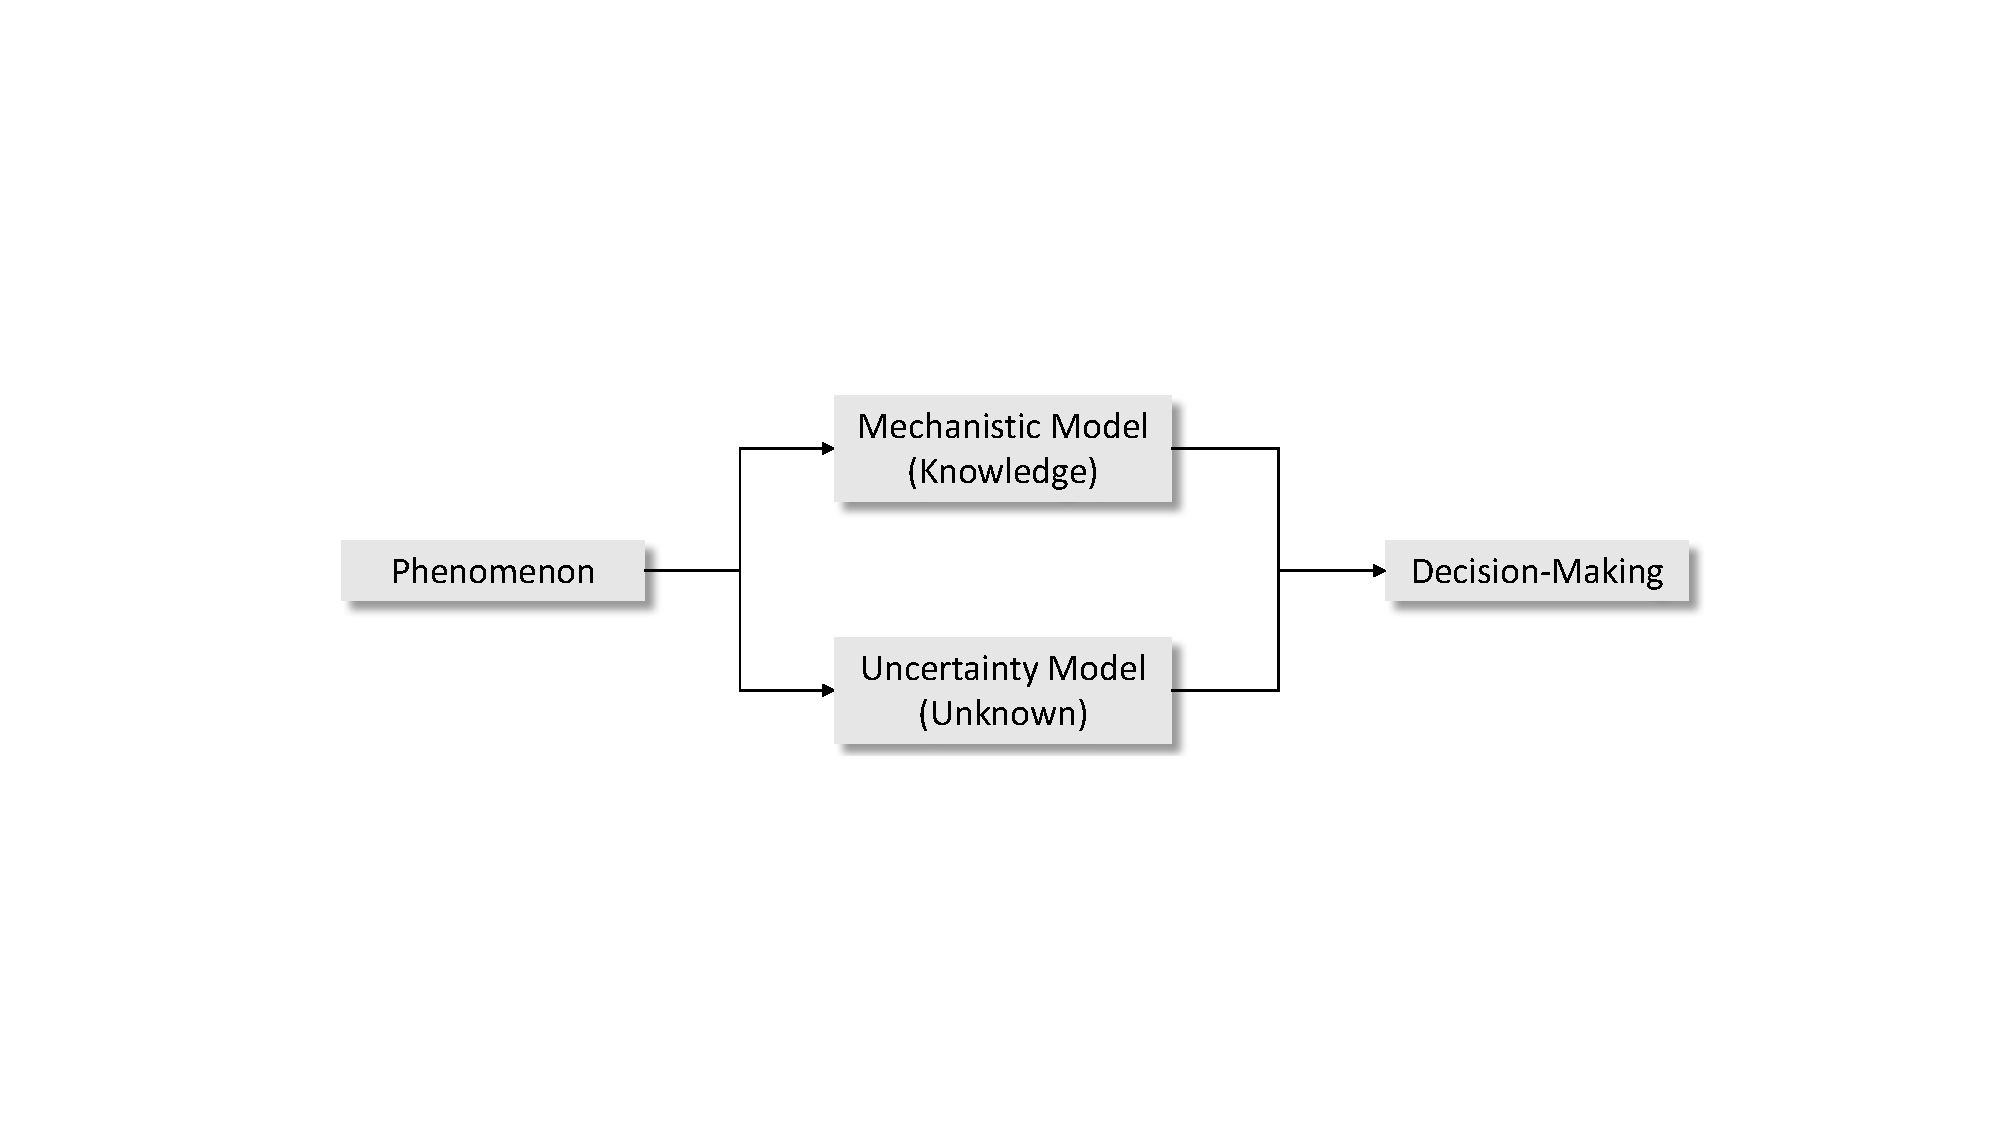
\includegraphics[width=0.7\textwidth]{figstats/phen_mech_rand}
\end{figure}
\
\end{frame}
%%------------------------------------------------


%
%%------------------------------------------------
\begin{frame}{Motivation}

{\em Statistics} is the branch of mathematics that offers tools to: 
\begin{itemize}
\item Collect, analyze, and extract knowledge (models) from data 
\item Characterize and model the unknown (uncertainty) 
\item Systematically make decisions in the face of uncertainty
\end{itemize}

\begin{block}{}
For an engineering perspective, {\em statistics} aids the discovery and development of mechanistic models and provides complementary (data-driven) modeling capabilities.  
\end{block}

\begin{block}{}
From a scientific perspective, {\em statistics} provides a way of thinking about the world that can help us understand how humans naturally process data to extract knowledge and to ultimately make decisions. 
\end{block}
\end{frame}
%%------------------------------------------------
%
%%%------------------------------------------------
\begin{frame}{Random Variables}
In statistics, we use random variables (RVs) to {\em model} uncertain behavior. An RV (denoted as $X$) does not have a known value and exhibits {\em variability} and has the following properties: 
\begin{block}{}
\begin{itemize}
\item An RV is characterized by a realization set $\omega \in \Omega$ with associated values $x_\omega\in \mathcal{D}_X$ (a.k.a. realizations of $X$).  Here, $\mathcal{D}_X$ is the domain of $X$.
\item An RV is characterized by a measure $\mathbb{P}:\Omega\to [0,1]$, which assigns probability to events (combinations of realizations); e.g., $\mathbb{P}(X\in \mathcal{A})$ for some $\mathcal{A}\subseteq \mathcal{D}_X$.
\end{itemize}
\end{block}
\end{frame}
%%------------------------------------------------

%%%------------------------------------------------
\begin{frame}{Random Variables}
\begin{block}{}
\begin{itemize}
\item The measure $\mathbb{P}$ has an associated cumulative density function (cdf) $F_X:\mathcal{D}_X\to [0,1]$. The cdf assigns a probability to the event that $X$ is below a certain threshold value $x$; i.e., $F_X(x)=\mathbb{P}(X\leq x)$.
\item The cdf has an associated probability density function (pdf) $f_X:\mathcal{D}_X\to [0,1]$. The pdf assigns a probability to the event that $X$ takes a specific value $x$; i.e., $f_X(x)=\mathbb{P}(X=x)$.  
\end{itemize}
\end{block}
An RV that has a unique and known value (exhibits no variability) is called a {\em deterministic variable}. 
\end{frame}
%%------------------------------------------------


%%%------------------------------------------------
\begin{frame}{Random Variables}
\begin{block}{}
{\bf Don't Forget:} A random variable is a {\em model} of a unknown phenomenon. 
\end{block}
\end{frame}
%%------------------------------------------------

%%%------------------------------------------------
\begin{frame}{Example: Gibbs Reactor}

\begin{itemize}
\item Consider a reactor under which the reaction $CO+2H_2\leftrightarrow CH_3OH$ takes place
\item Equilibrium and is favored by high pressure ($P$) and low temperature ($T$)
\item It has a control system to maintain $P$ and $T$ at desired conditions
\end{itemize}

\begin{columns}
\begin{column}{0.3\textwidth}
\begin{figure}[!htb]
    \centering
	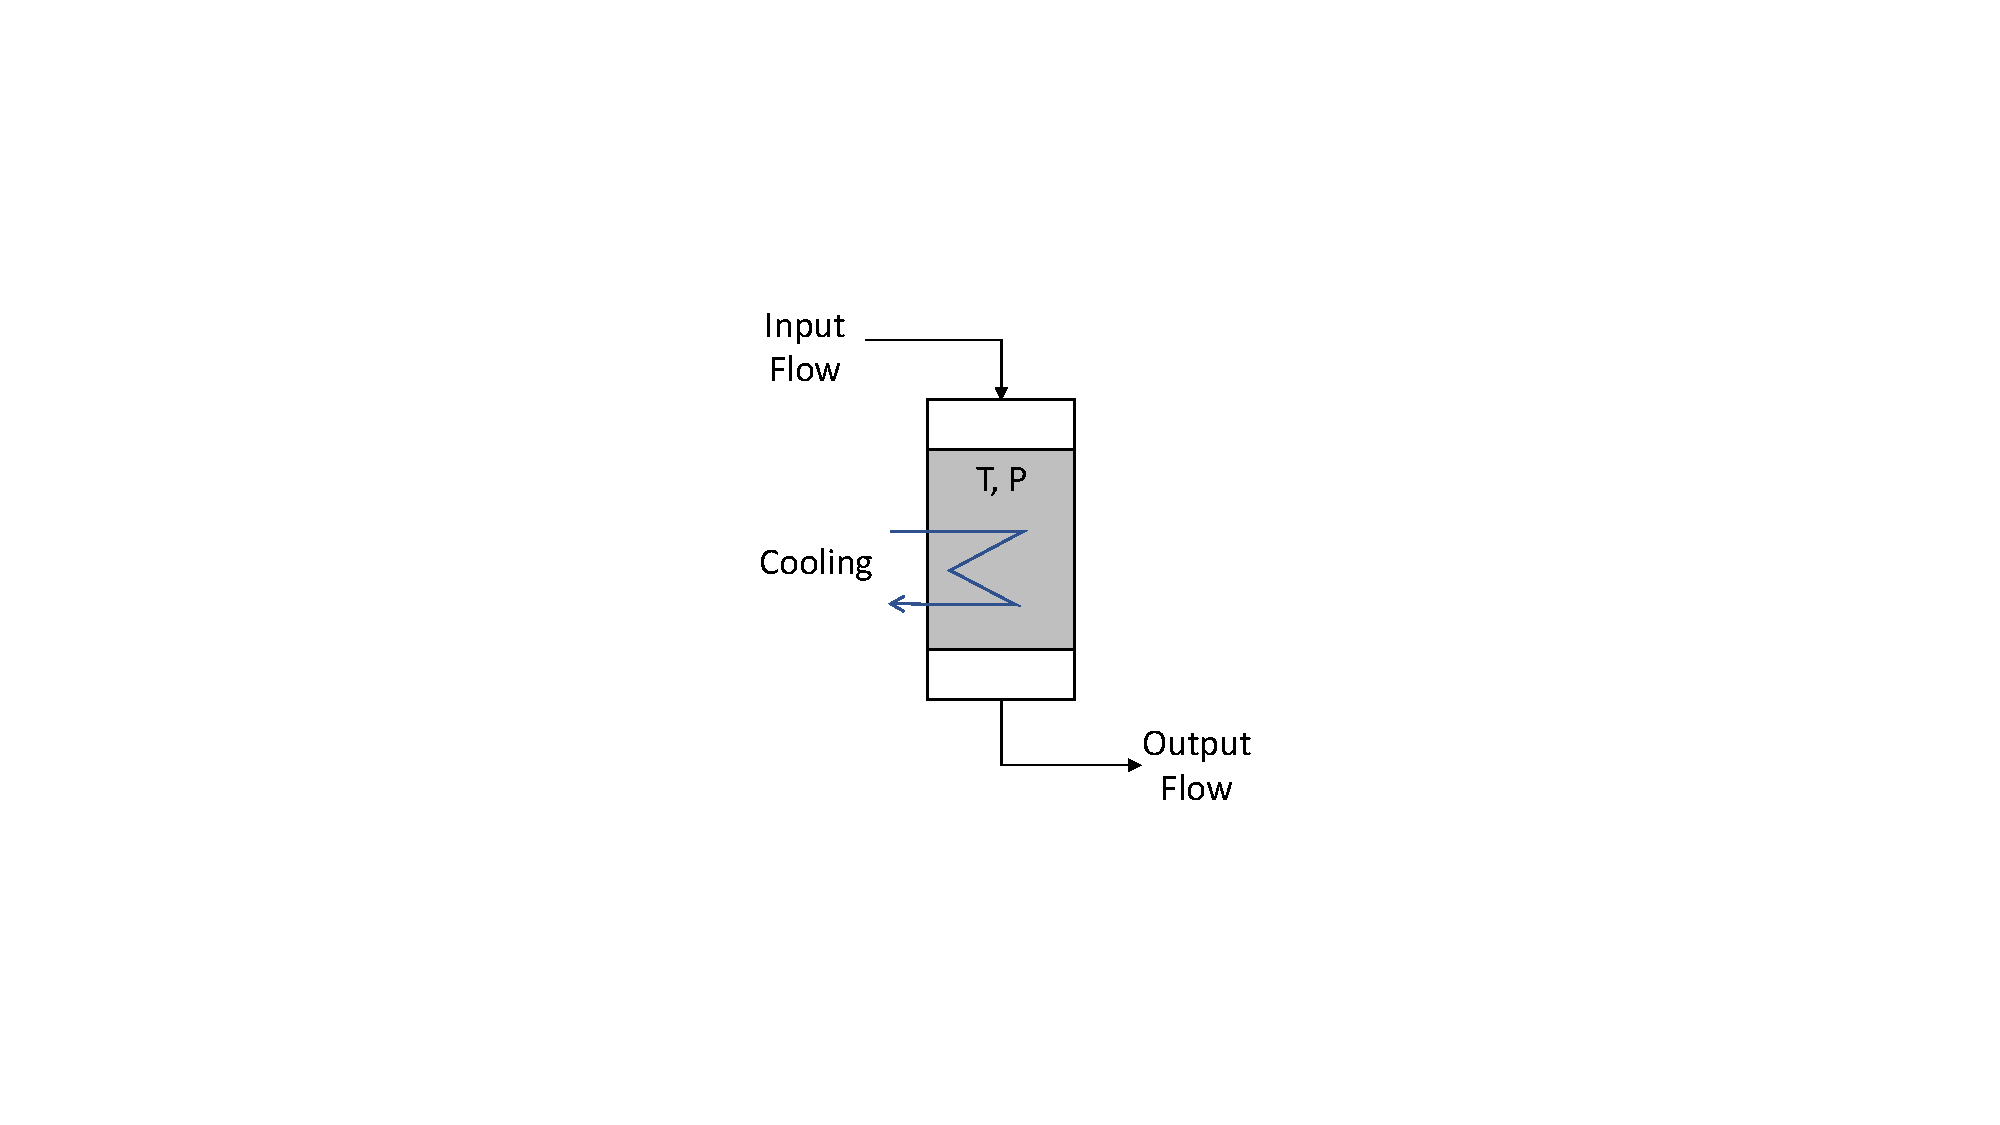
\includegraphics[width=\textwidth]{figstats/gibbs_diagram}
\end{figure}
\end{column}
\begin{column}{0.5\textwidth}
\begin{align*}
\mu_{out}^k&=\mu_{in}^k+\gamma^k\xi,\;k\in K\\
\mu_{tot}&=\sum_{k\in K}\mu_{out}^k\\
a^k&=\left(P\,\frac{\mu_{out}^k}{\mu_{tot}}\right)^{\gamma^k},\;k\in K\\
K_{eq}(T)&=\prod_{k\in K}a^k.
\end{align*}
\end{column}

\end{columns}


\begin{block}{}
\begin{itemize}
\item What is unknown (what are sources of randomness)?
\end{itemize}
\end{block}
\end{frame}
%%------------------------------------------------

%%%------------------------------------------------
\begin{frame}{Example: Gibbs Reactor}

\begin{itemize}
\item Assume {\em pressure} varies due to malfunction of control and model this as an RV
\item The outcomes, pdf, and cdf of RV are shown below. How do we interpret these? 
\end{itemize}
\begin{figure}[!htb]
    \centering
	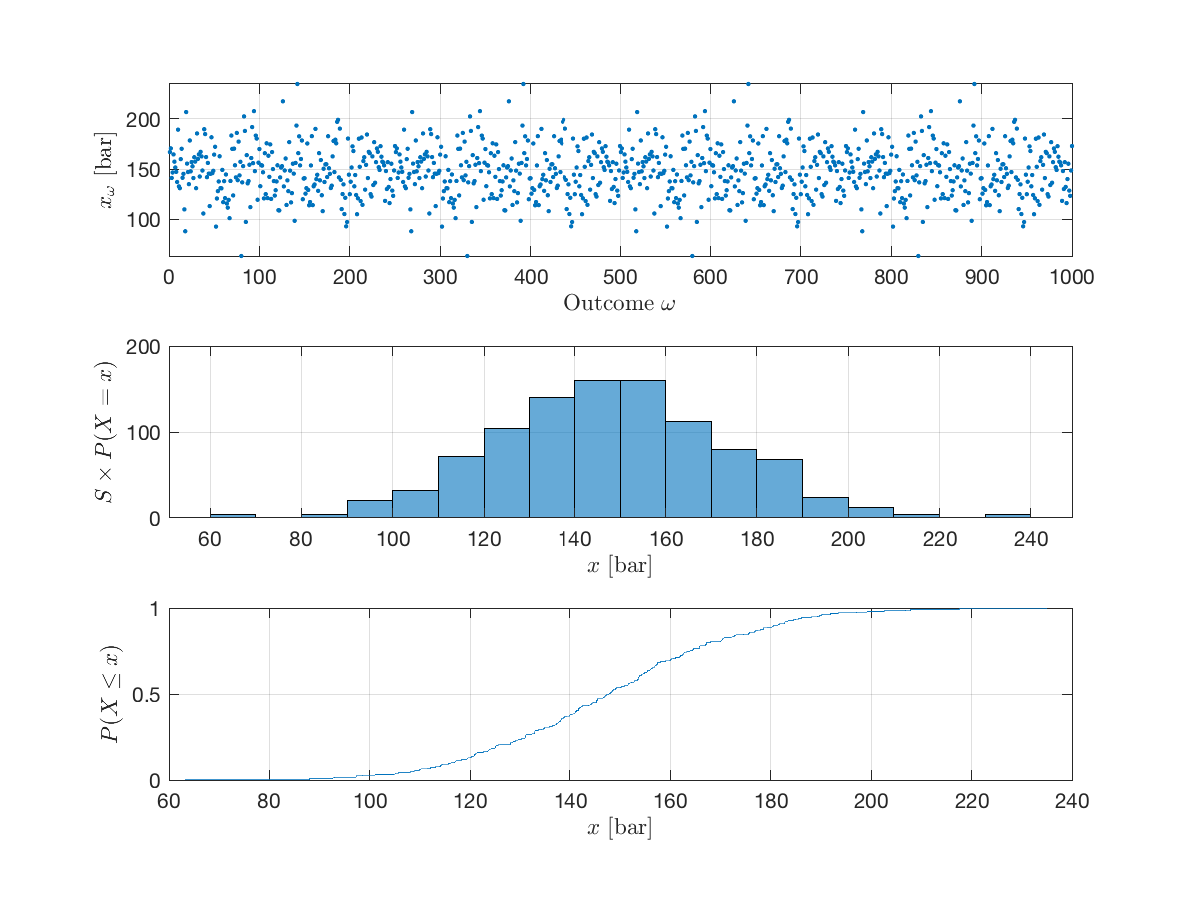
\includegraphics[width=0.8\textwidth]{figstats/Matlab/gibbs_press_pdf_cdf}
\end{figure}

\end{frame}
%%------------------------------------------------

%%%------------------------------------------------
\begin{frame}{Types of Random Variables}
RVs are categorized as multivariate vs. univariate and continuous vs. discrete:

\begin{block}{}
\begin{itemize}
\item A {\em multivariate} RV $X=(X_{1},X_{2},...,X_n)$ has realizations that are vector values $x_{\omega}=(x_{\omega,1},x_{\omega,2},...,x_{\omega,n})\in \mathbb{R}^n$; e.g., temperature and reaction conversion.
\item A {\em univariate} RV $X$ is a multivariate with $n=1$ and has realizations that are scalar values $x_\omega\in \mathbb{R}$; e.g., temperature.
\item A {\em continuous} RV $X$ is that in which the domain $\mathcal{D}_X$ is continuous; e.g., $X=(X_1,X_2)$ has realizations satisfying $0\leq x_{\omega,1}\leq 1$ and $0\leq x_{\omega,2}\leq 1$.
\item A {\em discrete} RV $X$ is that in which the domain $\mathcal{D}_X$ is discrete; e.g., $X=(X_1,X_2)$ has realizations satisfying $x_{\omega,1}\in \{0,1\}$ and $x_{\omega,2}\in \{0,1\}$.
\end{itemize}
\end{block}
There is a wide range of models of random variables that apply to the different categories (e.g., Gaussian is for continuous and Poisson for discrete). We will explore these later.  
\end{frame}
%%------------------------------------------------

%------------------------------------------------
%
\begin{frame}{Probability Density of Discrete and Continuous RVs}

A discrete RV $X$ has a discrete domain $\mathcal{D}_X$ and, as such, its pdf $f_X(x)$ is not a continuous function. Consequently:
\begin{block}{}

\begin{align*}
f(x)&\geq 0,\quad x\in \mathcal{D}_X\\
\sum_{x\in D_X}f(x)&=1\\
\mathbb{P}(X\in \mathcal{A})&=\sum_{x\in \mathcal{A}}f(x),\quad  \mathcal{A}\subseteq \mathcal{D}_X.
\end{align*}
\end{block}

A continuous RV $X$ has a continuous domain $\mathcal{D}_X$ and its pdf $f_X(x)$ is a continuous function. Consequently:
\begin{block}{}
\begin{align*}
f(x)&\geq 0,\quad x\in \mathcal{D}_X\\
\int_{x\in \mathcal{D}_X}f(x)dx&=1\\
\mathbb{P}(X\in \mathcal{A})&=\int_{x\in \mathcal{A}}f(x)dx,\quad  \mathcal{A}\subseteq \mathcal{D}_X.
\end{align*}
\end{block}



\end{frame}
%------------------------------------------------

%------------------------------------------------
%
\begin{frame}{Probability Density of Discrete and Continuous RVs}

\begin{itemize}
\item A discrete RV is easy to handle computationally  (involves summations):
\begin{itemize}
\item If $\mathcal{D}_X$ is discrete then $\mathbb{P}(X\leq a)=F_X(a)=\sum_{x\in \mathcal{D}_X}f_X(x)\mathbf{1}[x\leq a]$. 
\end{itemize}
Here, we use the indicator function $\mathbf{1}[x\leq a]=1$ if $x\leq a$ and $\mathbf{1}[x\leq a]=0$ if $x> a$. 

\item A continuous RV is difficult to handle computationally (involves integrals) but has useful properties that facilitate analysis:
\begin{itemize}
\item If $\mathcal{D}_X$ continuous then $\mathbb{P}(X\leq a)=F_X(a)=\int_{x\in \mathcal{D}_X}f_X(x)dx$. 
\item The cdf and pdf are related as $\frac{dF_X(x)}{dx}=f_X(x)$ and thus $\int_{x\in \mathcal{A}}f_X(x)dx=\int_{x\in \mathcal{A}}dF_X(x)$.
\end{itemize}

\item Continuous RVs are often approximated using discrete RVs (discretization). This is analogous to discrete time and continuous time. 

\end{itemize}


\end{frame}
%------------------------------------------------

%%------------------------------------------------
\begin{frame}{From Data to Random Variables}
We will begin our discussion by considering RVs that are {\em univariate}.
\begin{block}{}
\begin{itemize}
\item In practice, we often count with observations (data) for a given variable of interest $x_\omega,\, \omega \in \mathcal{S}$. Our objective is to use the data to model this variable as an RV. 
\item If we assume that $\mathcal{S}$ (a.k.a. sample set) is a subset of the realization set $\Omega$ (which is usually extremely large), we can construct a data-driven approximation (a.k.a. empirical or sample approximation) of the domain, cdf, and pdf of $X$.
\item The empirical domain $\hat{D}_X$ is the domain covered by the observations $x_\omega,\, \omega in \Omega$.
\item The ``theoretical" pdf is approximated using the empirical pdf: 
\begin{align*}
\hat{f}_X(x)=\frac{1}{S}\sum_{\omega \in \mathcal{S}}[x_\omega= x],\; x\in \hat{D}_X
\end{align*}
i.e., this is the frequency at which $X$ takes a value $x$ normalized by $S=|\mathcal{S}|$. 
\item The ``theoretical" cdf is approximated using the empirical cdf:
\begin{align*}
\hat{F}_X(x)=\frac{1}{S}\sum_{\omega \in \mathcal{S}}\mathbf{1}[x_\omega\leq x],\; x\in \hat{D}_X
\end{align*}
i.e., this is the frequency at which $X$ takes a value below $x$ normalized by $S=|\mathcal{S}|$. 
\end{itemize}
\end{block}
\end{frame}
%------------------------------------------------

%%%------------------------------------------------
\begin{frame}{Example: Gibbs Reactor}

\begin{itemize}
\item Here is a comparison of the empirical and theoretical pdfs and cdfs for pressure
\end{itemize}
\begin{figure}[!htb]
    \centering
	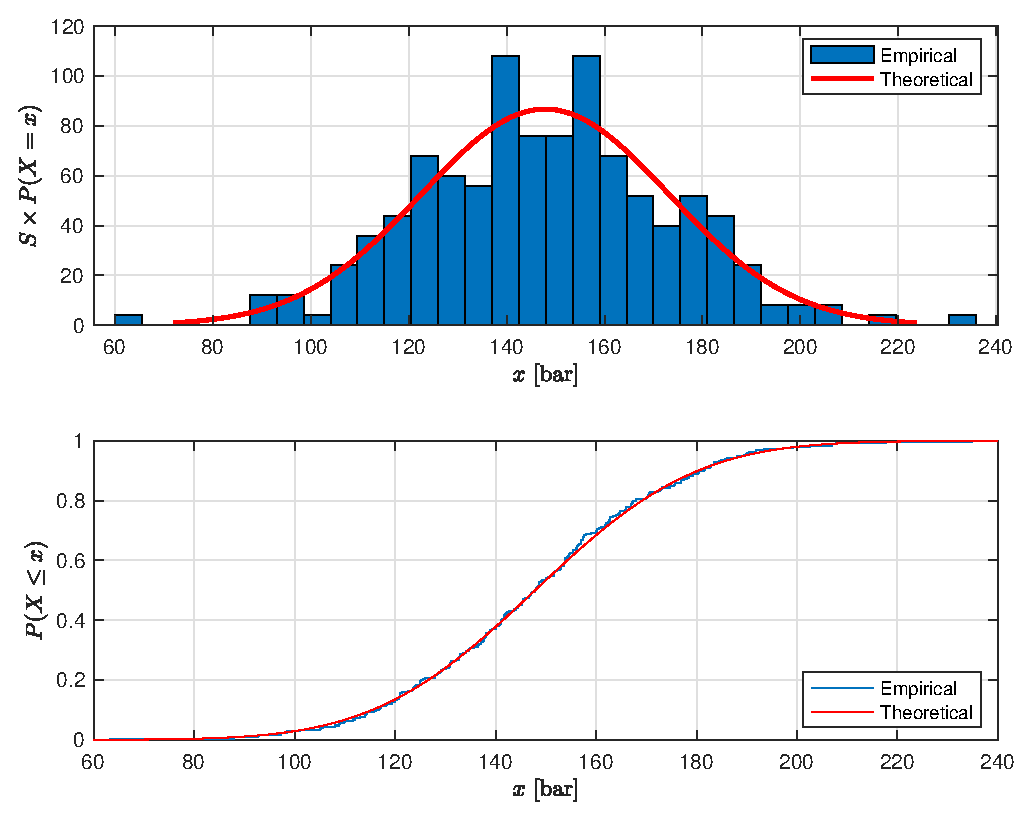
\includegraphics[width=0.7\textwidth]{figstats/Matlab/gibbs_press_pdf_cdf_fit}
\end{figure}

\end{frame}
%%------------------------------------------------

%------------------------------------------------
%
\begin{frame}{Summarizing Statistics (Basic)}
The pdf and cdf are {\em functions} that fully characterize an RV $X$. However, in practice, we might be interested in using scalar quantities and not functions.  This can be done by using summarizing statistics. 
\begin{block}{}
For a discrete RV we have:
\begin{itemize}
\item {\em Expected Value (measure of magnitude):} $\mathbb{E}_X:=\sum_{x\in {\mathcal{D}}_X}x{f}_X(x)$

\item {\em Variance and Standard Deviation (measure of variability):} 
\begin{align*}
\mathbb{V}_X:=\sum_{x\in {\mathcal{D}}_X}f_X(x)(x-\mathbb{E}_X)^2,\qquad \textrm{SD}_X:=\sqrt{\mathbb{V}_X}
\end{align*}
\end{itemize}
\end{block}

\begin{block}{}
For a continuous RV we have:
\begin{itemize}
\item {\em Expected Value (measure of magnitude):}  $\mathbb{E}_X:=\int_{x\in {\mathcal{D}}_X}x{f}_X(x)dx$
\item {\em Variance and Standard Deviation (measure of variability):} 
\begin{align*}
\mathbb{V}_X:=\int_{x\in {\mathcal{D}}_X}(x-\mathbb{E}_X)^2f_X(x)dx,\qquad \textrm{SD}_X:=\sqrt{\mathbb{V}_X}
\end{align*}
\end{itemize}
\end{block}
When convenient, we will use notation $\mathbb{E}[X]$ and $\mathbb{V}[X]$ to define summarizing statistics. 
\end{frame}
%------------------------------------------------

%------------------------------------------------
%
\begin{frame}{Summarizing Statistics (Sample Approximations)}
If we only have a finite set of data for $X$ available, we can approximate the summarizing statistics using their sample approximations: 
\begin{block}{}
\begin{itemize}
\item {\em Sample Mean (measure of magnitude):} 
\begin{align*}
\hat{\mathbb{E}}_X:=\sum_{x\in \hat{\mathcal{D}}_X}x\hat{f}_X(x)=\frac{1}{S}\sum_{\omega\in \mathcal{S}}x_\omega
\end{align*}
\item {\em Sample Variance and Standard Deviation (measure of variability):} 
\begin{align*}
\hat{\mathbb{V}}_X:=\sum_{x\in \hat{\mathcal{D}}_X}(x-\hat{E}_X)^2\hat{f}_X(x)=\frac{1}{S}\sum_{\omega\in \mathcal{S}}(x_\omega-\hat{E}_X)^2,\qquad \hat{\textrm{SD}}_X=\sqrt{\hat{\mathbb{V}}_X}
\end{align*}
\end{itemize}
\end{block}
Intuition tells us that these become better approximations as we accumulate data of $X$ (i.e., as $\mathcal{S}$ approaches $\Omega$). We will see later on that this is indeed the case. 
\end{frame}
%------------------------------------------------

%%%------------------------------------------------
\begin{frame}{Example: Gibbs Reactor}
\begin{itemize}
\item Here is behavior of sample mean and standard deviation as we increase sample size $S$
\end{itemize}
\begin{figure}[!htb]
    \centering
	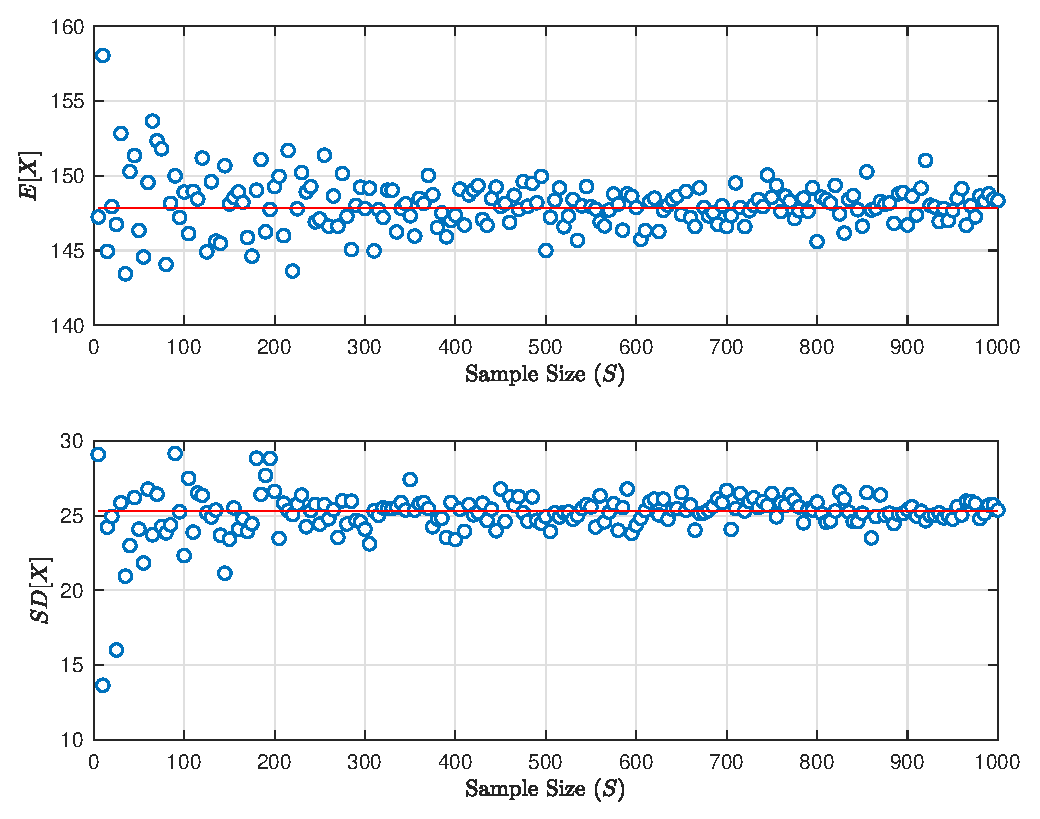
\includegraphics[width=0.7\textwidth]{figstats/Matlab/gibbs_press_exp_var}
\end{figure}

\end{frame}
%%%------------------------------------------------

%------------------------------------------------
%
\begin{frame}{Summarizing Statistics (Quantiles)}
An important family of summarizing statistics are the quantiles (a.k.a. percentiles). 
\begin{block}{}
\begin{itemize}
\item The quantile is the inverse function of the cdf and, as such, it might be easier to explain it from this perspective.  Consider the following equation for some $\alpha \in [0,1]$:
\begin{align*}
F_X(x)=\mathbb{P}(X\leq x)=\alpha 
\end{align*}
\item A value $x$ that satisfies this equation is the $\alpha$-quantile of the random variable $X$ and is denoted as $\mathbb{Q}_X(\alpha)$. This means that we can express the quantile as:
\begin{align*}
\mathbb{Q}_X(\alpha)=F^{-1}_X(\alpha) 
\end{align*}
\end{itemize}
\end{block}
\end{frame}
%------------------------------------------------

%------------------------------------------------
%
\begin{frame}{Summarizing Statistics (Quantiles)}
Some important observations about quantiles:
\begin{block}{}
\begin{itemize}
\item Since the cdf can have a ``staircase" form, there might be multiple values of $x$ satisfying $F_X(x)=\alpha$. Consequently, the $\alpha$-quantile might be not be unique. Typically,  the definition of the quantile is refined by looking for the smallest or center values of $x$ satisfying $F_X(x)\geq \alpha$. 

\item Quantiles are related to other summarizing statistics for interest. For instance: 
\begin{itemize}
\item $\mathbb{Q}_{X}(1/2)$ is the {\em center value} of $X$ (a.k.a. the median and denoted as $\mathbb{M}_X$)
\item $\mathbb{Q}_X(1)=\max_{x\in \mathcal{D}_X }x$ is the maximum value of $X$
\item $\mathbb{Q}_{X}(0)=\min_{x\in \mathcal{D}_X }x$ is the minimum value of $X$ 
\end{itemize}
\item We can use the empirical cdf $\hat{F}_X(x)$ to estimate empirical quantiles $\hat{\mathbb{Q}}(\alpha)$.
\end{itemize}
\end{block}
\end{frame}
%------------------------------------------------

%%------------------------------------------------
%%
\begin{frame}{Summarizing Statistic (Moments)}

\begin{itemize}
\item An important family of summarizing statistics are central moments. 

\item The moments of $X$ with pdf $f(x,\theta)$ are given by:
\begin{block}{}
\begin{align*}
m_k:=\mathbb{E}[(X-\mathbb{E}[X])^k], \qquad k=1,2,3,4,...,
\end{align*}
\end{block}
\item The normalized moments of $X$ with pdf $f(x,\theta)$ are given by:
\begin{block}{}
\begin{align*}
m_k:=\frac{\mathbb{E}[(X-\mathbb{E}[X])^k]}{SD[X]^k}, \qquad k=1,2,3,4,...,
\end{align*}
\end{block}

\item The first moment is simply $m_1=0$ while the second moment $m_2=\mathbb{V}[X]$ is the variance, the third moment $m_3$ is known as skewness, and the fourth moment  $m_4$ as kurtosis. 

\item As with the expectation and variance, we can use data to construct sample approximations for the moments $\hat{m}_k$. 

\end{itemize}

\end{frame}
%------------------------------------------------

%%%------------------------------------------------
\begin{frame}{Example: Gibbs Reactor}
\begin{itemize}
\item Sample moment approximations with $S=1000$ are $\hat{m}_1=0,\hat{m}_2=638$, $\hat{m}_3=1539$.
\item Theoretical are $\hat{m}_1=0,\hat{m}_2=639$, $\hat{m}_3=0$. What is going on with third moment?
\item Empirical and theoretical quantiles are shown below. How do we interpret this? 
\end{itemize}
\begin{figure}[!htb]
    \centering
	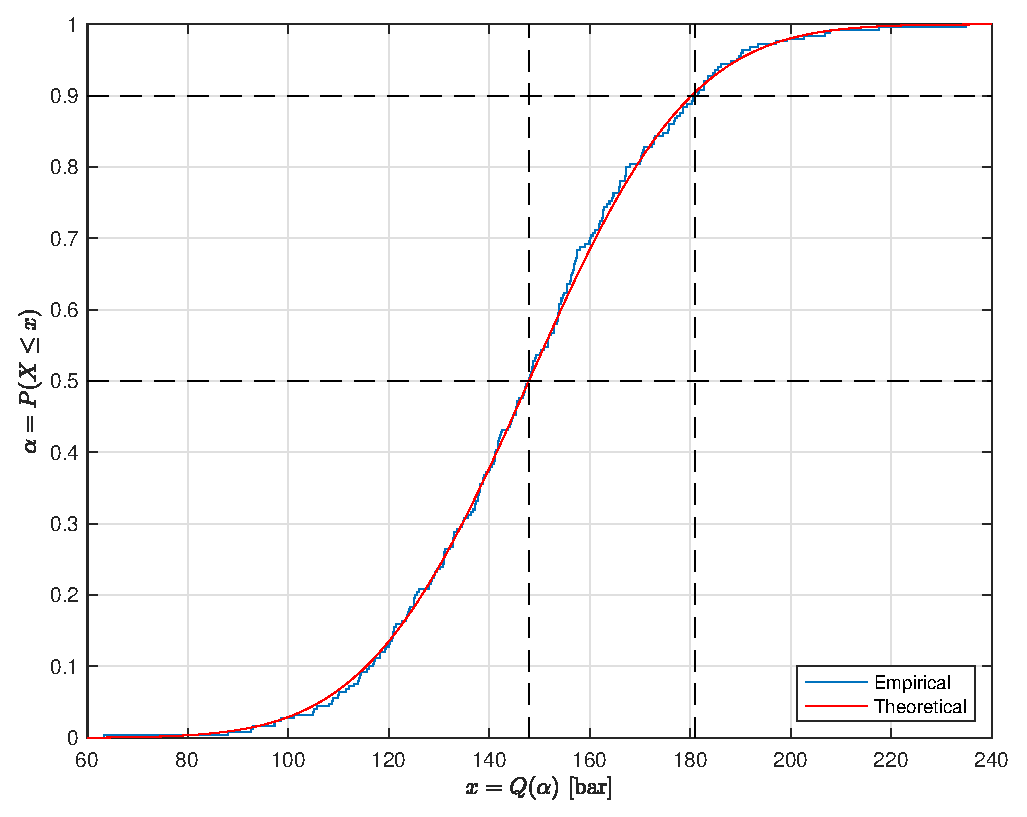
\includegraphics[width=0.6\textwidth]{figstats/Matlab/gibbs_press_quantile}
\end{figure}
\end{frame}
%%&------------------------------------------------

%------------------------------------------------
%
\begin{frame}{Uncertainty Propagation and Mitigation}
The uncertainty (and variability) associated with random variables propagate through systems in complex ways. Fortunately, we often have the ability to manipulate a system (through design or control) in order to mitigate the effects of this variability. 
\begin{block}{}
Consider the propagation of $X$ through a system described by a function $\varphi(X,u)$, where $u\in \mathcal{U}$ is an action (decision):
\begin{align*}
Y=\varphi(X,u)
\end{align*}
\end{block}
We make the following observations:
\begin{block}{}
\begin{itemize}
\item The output $Y$ is an RV if the input $X$ is an RV.
\item The nature of $Y$ (its cdf, pdf, and domain) depends on the system function $\varphi$. Some systems might magnify uncertainty and variability while others might damp it. 
\item The nature of $Y$ depends on the decision $u$.  We can implement actions on the system $\varphi$ to control the uncertainty and variability of $Y$.  
\end{itemize}
\end{block}
\end{frame}
%------------------------------------------------

%------------------------------------------------
%
\begin{frame}{Uncertainty Propagation and Mitigation}
Having data $x_\omega,\; \omega \in \mathcal{S}$ and a system $\varphi$, we can characterize the cdf, pdf, domain, and summarizing statistics of $Y$ using the following procedure. 
\begin{block}{}
\begin{itemize}
\item For a given $u$, perform simulations of the form:
\begin{align*}
y_\omega=\varphi(x_\omega,u),\; \omega \in \mathcal{S}
\end{align*} 
\item We use $y_\omega$ to compute approximations of quantities of interest for $Y$ such as:
\begin{itemize}
\item Sample mean:
\begin{align*}
 \hat{\mathbb{E}}_Y=\frac{1}{S}\sum_{\omega \in \mathcal{S}}y_\omega=\frac{1}{S}\sum_{\omega \in \mathcal{S}}\varphi(x_\omega,u)
 \end{align*}
\item Sample variance: 
\begin{align*}
\hat{\mathbb{V}}_Y=\frac{1}{S}\sum_{\omega \in \mathcal{S}}(y_\omega-\hat{\mathbb{E}}_Y)^2
\end{align*} 
\item Empirical cdf: 
\begin{align*}
\hat{F}_Y(y)=\frac{1}{S}\sum_{\omega \in \mathcal{S}}\mathbf{1}[y_\omega \leq y] 
\end{align*}
and quantiles $\hat{Q}_Y(\alpha)$.
\end{itemize}
\end{itemize}
\end{block}
\end{frame}
%------------------------------------------------

%%%------------------------------------------------
\begin{frame}{Example: Gibbs Reactor}
\begin{itemize}
\item Empirical pdf and cdf for pressure ($X$) and conversion ($Y$). What do you notice?
\end{itemize}
\begin{figure}[!htb]
    \centering
	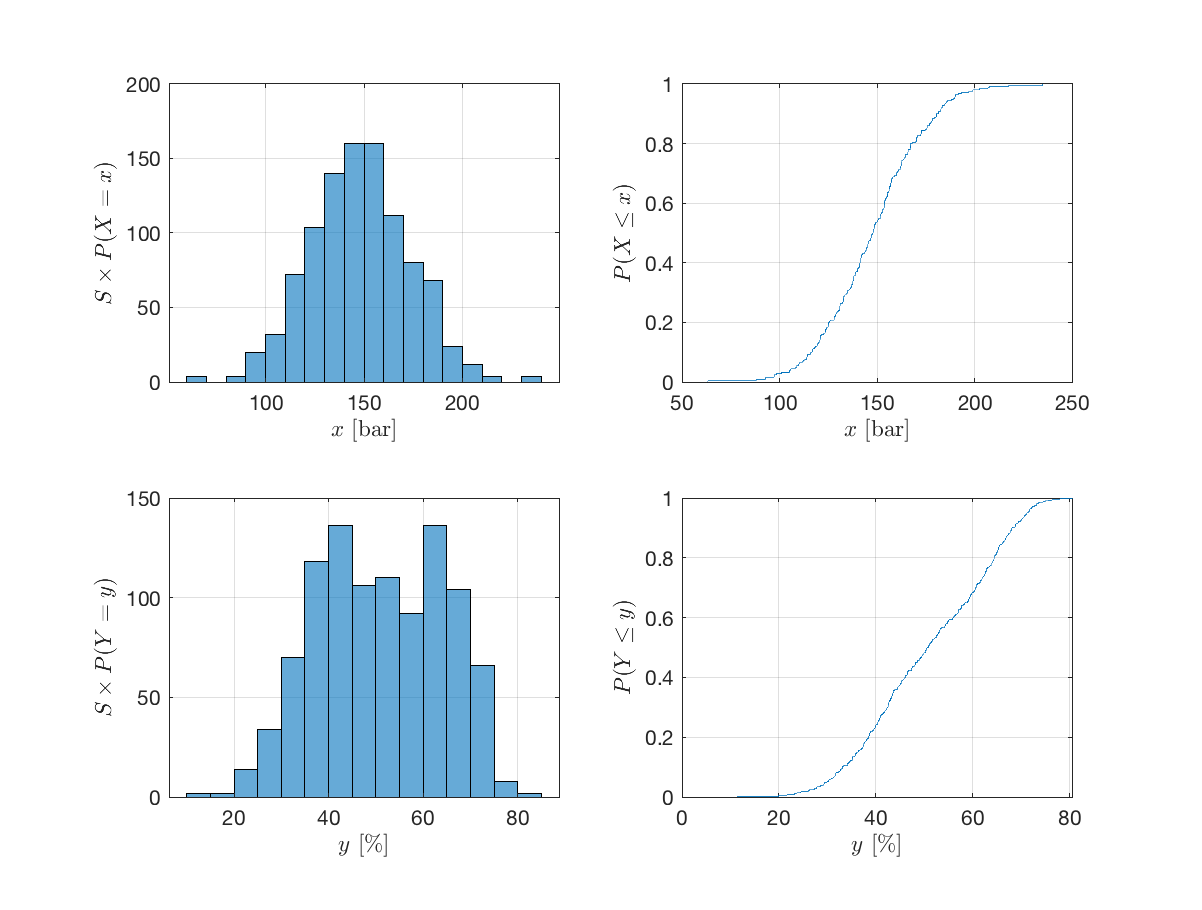
\includegraphics[width=0.8\textwidth]{figstats/Matlab/gibbs_press_extent}
\end{figure}

\end{frame}
%%%------------------------------------------------


%------------------------------------------------
%
\begin{frame}{Decision-Making under Uncertainty}
Consider now that we would like to find a decision $u\in \mathcal{U}$ that controls $Y(u)=\varphi(X,u)$ in some desirable way. This gives rise to a couple of questions:
\begin{block}{}
\begin{itemize}
\item If we have a couple of competing decisions $u$ and $u'$ giving rise to random outputs $Y(u)$ and $Y(u')$. How can we tell which one is better? 

\item How can we find the best possible decision $u$?
\end{itemize}
\end{block}
Some observations: 
\begin{itemize}
\item If we assume a {\em deterministic setting} with no uncertainty, then $Y(u)$ and $Y(u')$ will each take a single value and one would select, unambigously,  the one with the larger (or smaller) value. Mathematically, one would select $u$ if $Y(u)\geq Y(u')$.   

\item In a {\em setting under uncertainty} this is no longer possible because $Y(u)$ and $Y'(u)$ have multiple possible outcomes and with different probabilities. 

\item The concept of ``better" under uncertainty is ambiguous and the mathematical statement $Y(u)\leq Y(u')$ does not even make sense. Does $Y(u)\leq Y(u')$ mean that all the outcomes of $Y(u)$ are lower than those $Y(u')$? Does it mean that only a subset of outcomes is lower? 
\end{itemize}

\end{frame}
%------------------------------------------------

%%%------------------------------------------------
\begin{frame}{Example: Gibbs Reactor}
\begin{itemize}
\item Can counteract variability in pressure $X$ by operating at low or high temperature $u$
\item Compare empirical pdf and cdf for conversion at low $Y(u)$ and high temp $Y(u')$
\item Should we operate at low or high temperature?
\end{itemize}
\begin{figure}[!htb]
    \centering
	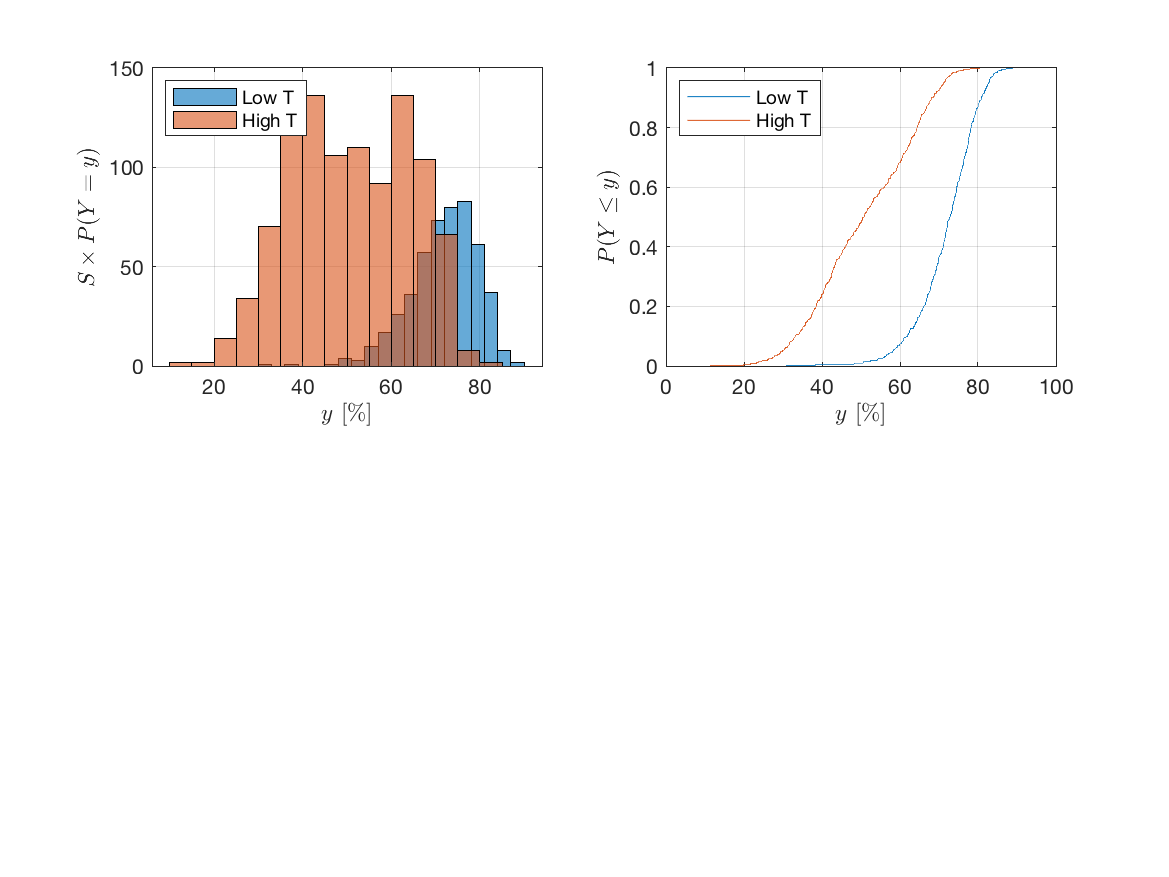
\includegraphics[width=\textwidth]{figstats/Matlab/gibbs_extent_temp}
\end{figure}

\end{frame}
%%%------------------------------------------------

%------------------------------------------------
%
\begin{frame}{Estimation}

Given that we have data $x_\omega, y_\omega,\; \omega \in \mathcal{S}$ available, we now place our attention to the following questions:
\begin{block}{}
Is the data following a particular pattern (trend)? If there is a pattern, can we model it? 
\end{block}
In this context, by a model, we mean two things: 
\begin{itemize}
\item If we have empirical statistics (e.g., cdf, pdf, mean, variance) obtained from data $x_\omega,y_\omega$, do these match the statistics of a {\em known} RV?
\item If we do not know the system model $\varphi$ that relates $x_\omega$ and $y_\omega$, can we determine this by using input-output data? 
\end{itemize}
The task of determining models from data is known as {\em estimation}. 

Having a model will allow us:
\begin{block}{}
\begin{itemize}
\item Determine if the available data is sufficient to say something meaningful about events that have not been observed (e.g., need more data to make a decision?). 
\item Make predictions about other possible events and their respective probabilities (e.g., how likely is an extreme event from happening?)
\item Extract trends that help us summarize the data available (from data to knowledge). 
\end{itemize}
\end{block}
Our first step is to postulate an RV model and see if this fits the data. 
\end{frame}
%------------------------------------------------



%------------------------------------------------
%
\begin{frame}{Model of a Gaussian RV}

\begin{itemize}

\item A wide range of RV models have been developed over the years based on identification of common patterns that emerge in real-life phenomena. 

\item Many phenomena follow the behavior of a normal RV (a.k.a. Gaussian RV). 

\end{itemize}

\begin{block}{}
A Gaussian RV is continuous and has an associated pdf:
\begin{align*}
f_X(x)=\frac{1}{\sqrt{2\pi\sigma^2}}e^{\frac{-(x-\mu)^2}{2\sigma^2}}, \quad  x\in \mathcal{D}_X=\{-\infty\leq x\leq \infty\}
\end{align*}
\end{block}
\begin{itemize}
\item The scalar values $\mu\in \mathbb{R},\sigma\in \mathbb{R}$ are hyperparameters that are specific to the application of interest. These are the values that we will seek to tune to match the model to the available data. 

\item We express the fact that an RV $X$ is Gaussian as $X\sim \mathcal{N}(\mu,\sigma^2)$. 

\end{itemize}

\end{frame}
%------------------------------------------------

%------------------------------------------------
%
\begin{frame}{Model of a Gaussian RV}


\begin{itemize}
\item The pdf tells us the behavior of the Gaussian RV: 
\begin{itemize}
\item the probability of an outcome $x$ decays exponentially fast as we move from $\mu$
\item the outcome of maximum probability (most likely outcome) is $\mu$
\item the speed of the decay is dictated by $\sigma$
\item the decay in probability is symmetric around $\mu$
\end{itemize}

\item Gaussian model assumes that an outcome $x$ can take any value in $(-\infty,\infty)$. This introduces complications, as many phenomena involves variables that cannot take negative values (e.g., mass) or infinite values (e.g., temperatures).   

\item Gaussian RVs can model a wide range of phenomena (e.g., diffusion). Moreover, many phenomena have the Gaussian RV as a limiting case (we will show this later). 
\end{itemize}

\end{frame}
%------------------------------------------------

%------------------------------------------------
%
\begin{frame}{Model of a Gaussian RV}
\begin{itemize}
\item Here are the pdfs for $\mathcal{N}(\mu,\sigma)$ for different values of $\mu$ and $\sigma$.
\item What do you observe?
\item What happens when $\sigma^2\to 0$?
\end{itemize}
\begin{figure}[!htb]
    \centering
	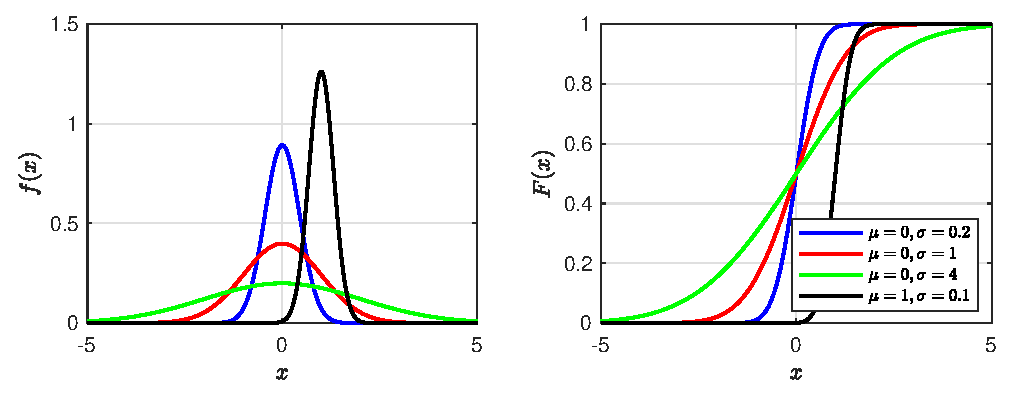
\includegraphics[width=\textwidth]{figstats/Matlab/gaussians}
\end{figure}
\end{frame}
%------------------------------------------------

%------------------------------------------------
%
\begin{frame}{Example: Diffusion Phenomena}
\begin{itemize}
\item Gaussian RV naturally emerges in diffusion phenomena
\item Consider question: What is probability of finding a particle in a particular location $x$ in the spatial domain $ [-\infty,\infty]$ and at a given time $t\in [0,T]$?
\item One can show that such probability, denotes as $f(x,t)$ solves the diffusion equation:
\begin{align*}
\frac{\partial f(x,t)}{\partial t}=D\frac{\partial^2 f(x,t)}{\partial x^2}
\end{align*}
with boundary conditions:
\begin{align*}
f(x,t)=0\; x\in [-\infty,\infty]\\
\int_{-\infty}^{\infty}f(x,t)dx=1,\quad t\in [0,T]
\end{align*}
\item The solution is:
\begin{align*}
f(x,t)=\frac{1}{\sqrt{4 \pi D t}}e^{-\frac{x^2}{4Dt}},\quad x\in [-\infty,\infty],\; t\in [0,T]
\end{align*}
\item Define dispersion coefficient $\sigma^2=2Dt$ and write:
\begin{align*}
f(x)=\frac{1}{\sqrt{2 \pi \sigma^2}}e^{-\frac{x^2}{2\sigma^2}},\quad  x\in [-\infty,\infty]
\end{align*}
\item That is position $X$ is random and given by $X\sim\mathcal{N}(0,\sigma^2)$ 
\item How does probability change with diffusivity $D$?
\end{itemize}

\end{frame}
%------------------------------------------------


%------------------------------------------------
%
\begin{frame}{Properties of a Gaussian RV}

A Gaussian RV $X\sim \mathcal{N}(\mu,\sigma^2)$ has many useful properties. For instance:
\begin{block}{}
\begin{itemize}
\item It expected value and variance are $\mathbb{E}_X=\mu$ and $\mathbb{V}[X]=\sigma^2$. 
\item Any linear transformation $Y=a+bX$ yields a Gaussian RV $Y\sim \mathcal{N}(a+b\mu,b^2\sigma^2)$. This implies that $\mathbb{E}_Y=a+b\mathbb{E}_X$ and $\mathbb{V}_Y=b^2\mathbb{V}_Y$. 
\item The cdf of $Y=a+bX$ satisfies $F_Y(y)=F_X(x)$ for all $y=a+bx$. 
\end{itemize}
\end{block}
Think about the implications of the above properties from an estimation and uncertainty propagation perspective: 
\begin{block}{}
\begin{itemize}
\item We can estimate  $\mu$ and $\sigma$ from data simply as $\mu =\hat{\mathbb{E}}_X$ and $\sigma^2=
\hat{\mathbb{V}}[X]$. This is sufficient to create our empirical Gaussian model. 
\item Any linear system $\varphi(X)=a+bX$ will generate a Gaussian RV as output if the input $X$ is linear. Moreover, the system will shrink the variability of $X$ if $b<1$ and will magnify if $b>1$. 
\end{itemize}
\end{block}

\end{frame}
%------------------------------------------------

%%%------------------------------------------------
\begin{frame}{Example: Mixing Problem}
\begin{itemize}
\item We have an input flow  $F_1=10$ (gpm) that can be measured with high accuracy to the point that it is OK to assume this to be deterministic. 
\item We have another input flow $F_2$ (gpm) that cannot be measured with high accuracy and is thus modeled as an RV $\mathcal{N}(20,1)$. This flow can be controlled using a valve with coefficient $\kappa \in [0,1]$. 
\end{itemize}
\begin{block}{}
\begin{itemize}
\item What type of RV is the output flow $F_3=F_1+\kappa\cdot F_2$? What is its mean and std dev?
\item How does uncertainty in $F_3$ change $\kappa\to 0$ and $\kappa\to 1$? Why?
\end{itemize}
\end{block}
\begin{figure}[!htb]
    \centering
	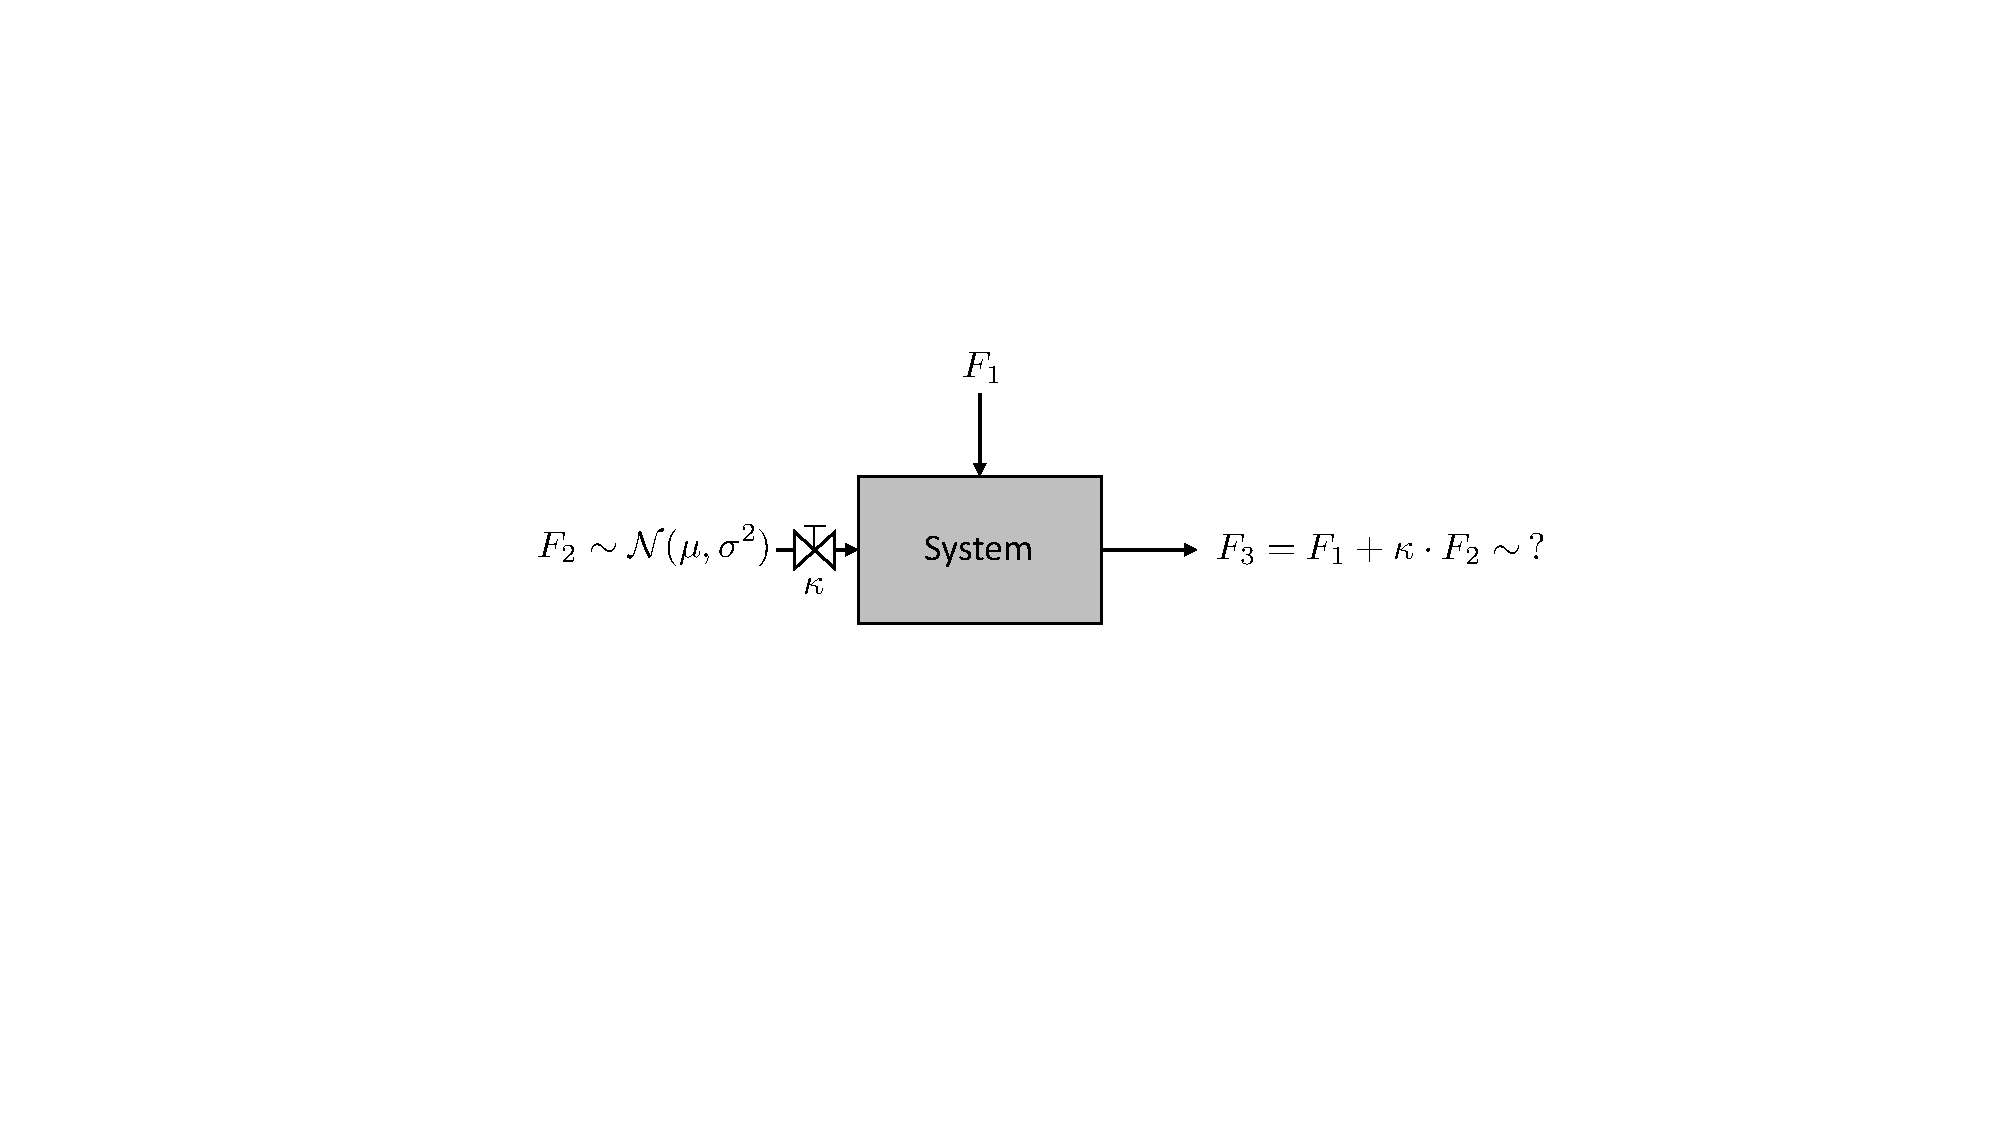
\includegraphics[width=0.7\textwidth]{figstats/mixing_diagram}
\end{figure}
\begin{itemize}
\item We have that $F_3=10+\kappa F_2$ and is thus $F_3$ a linear transformation of $F_2$
\item We thus have that $F_3\sim\mathcal{N}(10+\kappa\cdot 20,\kappa^2\cdot 1)$
\end{itemize}
\end{frame}
%%%------------------------------------------------


%------------------------------------------------
%
\begin{frame}{Properties of a Gaussian RV}

The cdf of a Gaussian RV is given by:
\begin{block}{}
\begin{align*}
F_X(x)=\frac{1}{2}\left(1+\textrm{erf}\left(\frac{(x-\mu)/\sigma}{\sqrt{2}}\right)\right)\; 
\end{align*}
where $\textrm{erf}:\mathbb{R}\to \mathbb{R}$ is the error function:
\begin{align*}
\textrm{erf}\left(\frac{(x-\mu)/\sigma}{\sqrt{2}}\right)=\frac{2}{\sqrt{\pi}}\int_0^{\frac{(x-\mu)/\sigma}{\sqrt{2}}}e^{-t^2}dt
\end{align*}
\end{block}
Computing the cdf involves evaluating an integral that depends on $\mu$ and $\sigma$. 

\end{frame}
%------------------------------------------------


%------------------------------------------------
%
\begin{frame}{Properties of a Gaussian RV}

\begin{itemize}
\item Fortunately, one can exploit properties of Gaussian RVs to avoid this issue. 

\item Note that $Z=(X-\mu)/\sigma$ is a linear transformation of $X\sim \mathcal{N}(\mu,\sigma^2)$ and and thus $Z\sim \mathcal{N}(0,1)$. 

\item Now note that the pdf and cdf of $Z$ are simply:
\begin{block}{}
\begin{align*}
f_Z(z)&=\frac{1}{\sqrt{2\pi}}e^{-\frac{1}{2}z^2}\\
F_Z\left(z\right)&=\frac{1}{2}\left(1+\textrm{erf}\left(\frac{z}{\sqrt{2}}\right)\right),\; \quad \textrm{erf}\left(\frac{z}{\sqrt{2}}\right)=\frac{2}{\sqrt{\pi}}\int_0^{\frac{z}{\sqrt{2}}}e^{-t^2}dt
\end{align*}
\end{block}
which do not depend on hyperparameters; $Z$ is known as the standard normal RV. 
\end{itemize}

\end{frame}
%------------------------------------------------


%------------------------------------------------
%
\begin{frame}{Properties of a Gaussian RV}

\begin{itemize}
\item From linear transfomation properties we have that $F_X(x)=F_Z(z)$ holds for any $z=(x-\mu)/\sigma$ and thus we can evaluate $F_X(x)$ at a given value $x$ by transforming $x$ into $z$ and then evaluate $F_Z(z)$. 

\item Since $F_Z(z)$ does not depend on any parameters, it can be precomputed (values of $F_Z(z)$ are available in software packages). 

\item If we want to compute $Q_X(\alpha)=F^{-1}_X(\alpha)$. As with cdf, we can compute this by using pre-computed quantiles of $Z$, which we denote as $z_\alpha:=F_Z^{-1}(\alpha)$. 

\item Relationship between the quantiles of $X$ and $Z$ is obtained directly from the linear transformation $x=\mu+\sigma z$:
\begin{align*}
Q_X(\alpha)=\mu+\sigma z_\alpha.
\end{align*}
The values $z_\alpha$ are known as the critical values of the standard normal. As with the cdf, these values have been precomputed and are available in software packages. 
\end{itemize}

\end{frame}
%------------------------------------------------

%%%------------------------------------------------
\begin{frame}{Example: Mixing Problem}
\begin{itemize}
\item Consider $\kappa=1$ and thus flow $F_3\sim\mathcal{N}(30,1)$
\item Quantile functions for  $\mathcal{N}(0,1)$ and $\mathcal{N}(30,1)$ are shown below
\end{itemize}
\begin{figure}[!htb]
    \centering
	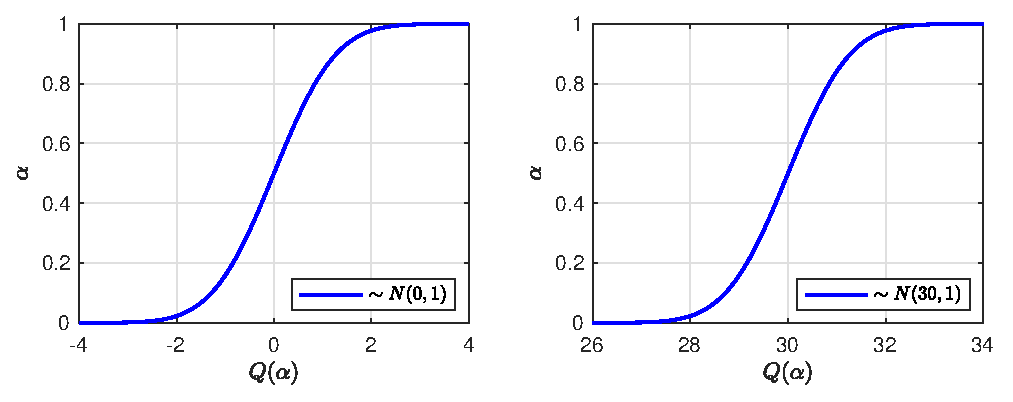
\includegraphics[width=0.8\textwidth]{figstats/Matlab/mixing_gauss}
\end{figure}
\begin{itemize}
\item Quantile of $\mathcal{N}(0,1)$ at $\alpha=0.977$ is  $Q(\alpha)=2$
\item Quantile of  $\mathcal{N}(\mu,\sigma)$ should be $\mu+2\cdot \sigma=32$.  Confirm this is true from plot
\end{itemize}
\end{frame}
%%%------------------------------------------------

%------------------------------------------------
%
\begin{frame}{Properties of a Gaussian RV}

\begin{itemize}
\item Standarization allows us to easily determine probability that $X$ is in specific ranges.

\item Imagine that you precomputed $F_Z(k)=\mathbb{P}(Z\leq k)$ for $k=0,1,2,3,...$. We have:
\begin{block}{}
\begin{align*}
\mathbb{P}(Z\leq 0)=50.0\%&\Longleftrightarrow\mathbb{P}(X\leq \mu)=50.0\%\\
\mathbb{P}(Z\leq 1)=84.1\%&\Longleftrightarrow\mathbb{P}(X\leq \mu+\sigma)=84.1\%\\
\mathbb{P}(Z\leq 2)=97.7\%&\Longleftrightarrow\mathbb{P}(X\leq \mu+2\sigma)=97.7\%\\
\mathbb{P}(Z\leq 3)=99.9\%&\Longleftrightarrow\mathbb{P}(X\leq \mu+3\sigma)=99.9\%
\end{align*}
\end{block}
\item i.e., the probability that $X$ is below its mean $\mu$ plus one $\sigma$ is always 84.1\%, the probability that it is below $\mu$ plus three $\sigma$ is always 99.9\% and so on.  
\end{itemize} 

\end{frame}
%------------------------------------------------

%------------------------------------------------
%
\begin{frame}{Properties of a Gaussian RV}

\begin{itemize}
\item Standarization allows us to easily determine {\em confidence regions} for $X$.

\item Assume a probability level $\alpha \in [0,1]$; we can show that critical value $z$ satisfying
\begin{align*}
\mathbb{P}(-z\leq Z\leq z)=1-\alpha
\end{align*}
is $z=F_Z^{-1}(1-\frac{\alpha}{2})$ (we denote this as $z_{1-\frac{\alpha}{2}}$). 
\item In other words, we have that:
\begin{align*}
\mathbb{P}(-z_{1-\frac{\alpha}{2}}\leq Z\leq z_{1-\frac{\alpha}{2}})=1-\alpha
\end{align*} 
\item Using the linear transformation property we obtain:
\begin{align*}
\mathbb{P}(\mu-z_{1-\frac{\alpha}{2}}\sigma\leq X\leq \mu+z_{1-\frac{\alpha}{2}}\sigma)=1-\alpha.
\end{align*}
\item i.e.; the probability of finding $X\sim\mathcal{N}(\mu,\sigma^2)$ in region $\mu\pm z_{1-\frac{\alpha}{2}}\sigma$ is $1-\alpha$. 
\item This gives an idea of how confident we are of finding $X$ in a given region; conversely, can also determine region under which we can find $X$ with a desired confidence. 
\item The concept of the confidence region is important in many topics of statistics. 
\end{itemize}
\end{frame}
%------------------------------------------------

%%%------------------------------------------------
\begin{frame}{Example: Mixing Problem}
\begin{itemize}
\item In what interval do we expect flow $F_3\sim\mathcal{N}(30,1)$ to be with 90\% probability? 
\end{itemize}
\begin{figure}[!htb]
    \centering
	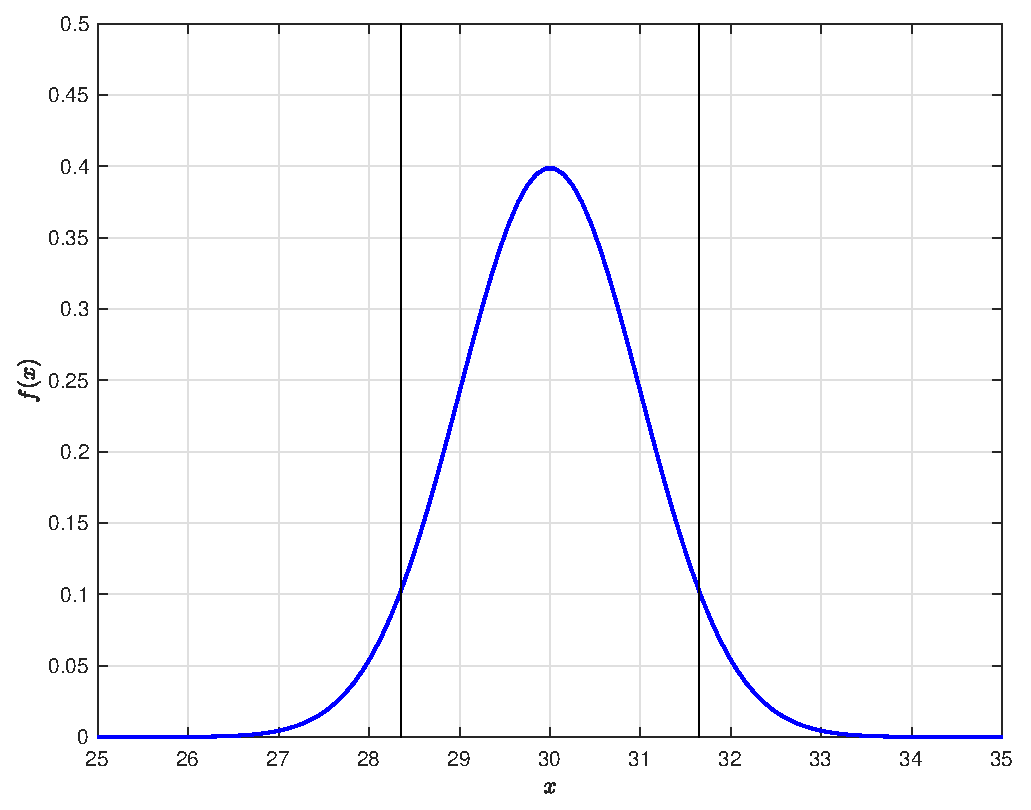
\includegraphics[width=0.6\textwidth]{figstats/Matlab/conf_mixing}
\end{figure}
\begin{itemize}
\item We have $1-\alpha=0.9$ and thus $\alpha=0.1$ and quantile for $Q(1-\frac{\alpha}{2})=1.644$.
\item We thus have $F_3\in [30-1.64\cdot 1,30+1.64\cdot 1]=[28.36,31.64]$ with 90\% prob. 
\end{itemize}
\end{frame}
%%%------------------------------------------------

%------------------------------------------------
%
\begin{frame}{Model of an Exponential RV}

Another RV that often appears in applications is the exponential random variable.  

\begin{block}{}
An exponential RV is continuous and has a pdf of the form:
\begin{align*}
f_X(x)=\frac{1}{\beta}e^{-x/\beta},\quad x\in \mathcal{D}_X=\{0\leq x\leq \infty\}.
\end{align*}
\end{block}
\begin{itemize}
\item The only hyerparameter of this model is $\beta \in \mathbb{R}_+$ (a.k.a. scale value). 
\item The reciprocal $\eta=1/\beta$ is known as the intensity and thus the pdf can also be written as $f_X(x)=\eta e^{-\eta\cdot x}$. 
\item We express the fact that $X$ is exponential as $X\sim \textrm{Exp}(\beta)$.
\end{itemize}

\end{frame}
%------------------------------------------------

%------------------------------------------------
%
\begin{frame}{Model of an Exponential RV}

\begin{itemize}
\item Pdf of the exponential RV tell us that:
\begin{itemize} 
\item Probability of finding $x$ away from zero decays exponentially fast at rate $\eta$
\item There is zero probability of finding $X$ below zero (pdf is asymmetric). One can think of an exponential RV as one side of a Gaussian RV. 
\end{itemize}
\item Cdf is $F_X(x)=1-e^{-x/\beta}$, expected value and variance are $\mathbb{E}_X=\beta$ and $\mathbb{V}_X=\beta^2$.
\item This RV is often used to model time phenomena associated with {\em failures}. 
\item For instance, $X$ can be used to model the amount of time that we have to wait until we observe the first occurrence of an event (e.g., engine fails). In this context, we know the average time that we have to wait ($\mathbb{E}_X=\beta$) but the actual time is random (unknown). 
\end{itemize}

\end{frame}
%------------------------------------------------

%------------------------------------------------
%
\begin{frame}{Model of an Exponential RV}
\begin{itemize}
\item Below at the pdfs and cdfs for $\textrm{Exp}(\beta)$ for different values of $\beta$.
\end{itemize}
\begin{figure}[!htb]
    \centering
	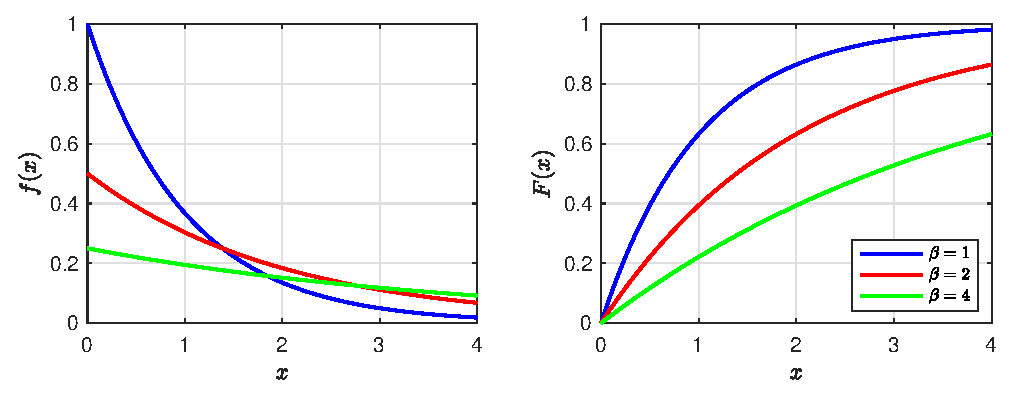
\includegraphics[width=0.8\textwidth]{figstats/Matlab/exponentials}
\end{figure}
\begin{block}{}
\begin{center}
How to determine $\beta$ from cdf? 
\end{center}
\end{block}
\pause
\begin{itemize}
\item Note that $F_X(x)=1-e^{-1}=0.63$ when $x=\beta$. 
\end{itemize}
\end{frame}
%------------------------------------------------

%------------------------------------------------
%
\begin{frame}{Example: Residence Time in Mixing System}
\begin{itemize}
\item  Mixed system with volume $V$ with input and output flow $F$
\item At time $t=0$ we inject particles so that input concentration is $C_0$.
\item The particle concentration in system at time $t$ is $C(t)$
\end{itemize}
\begin{block}{}
For how long will a particle reside in the system?  What factors influence this time? 
\end{block}
\begin{figure}[!htb]
    \centering
	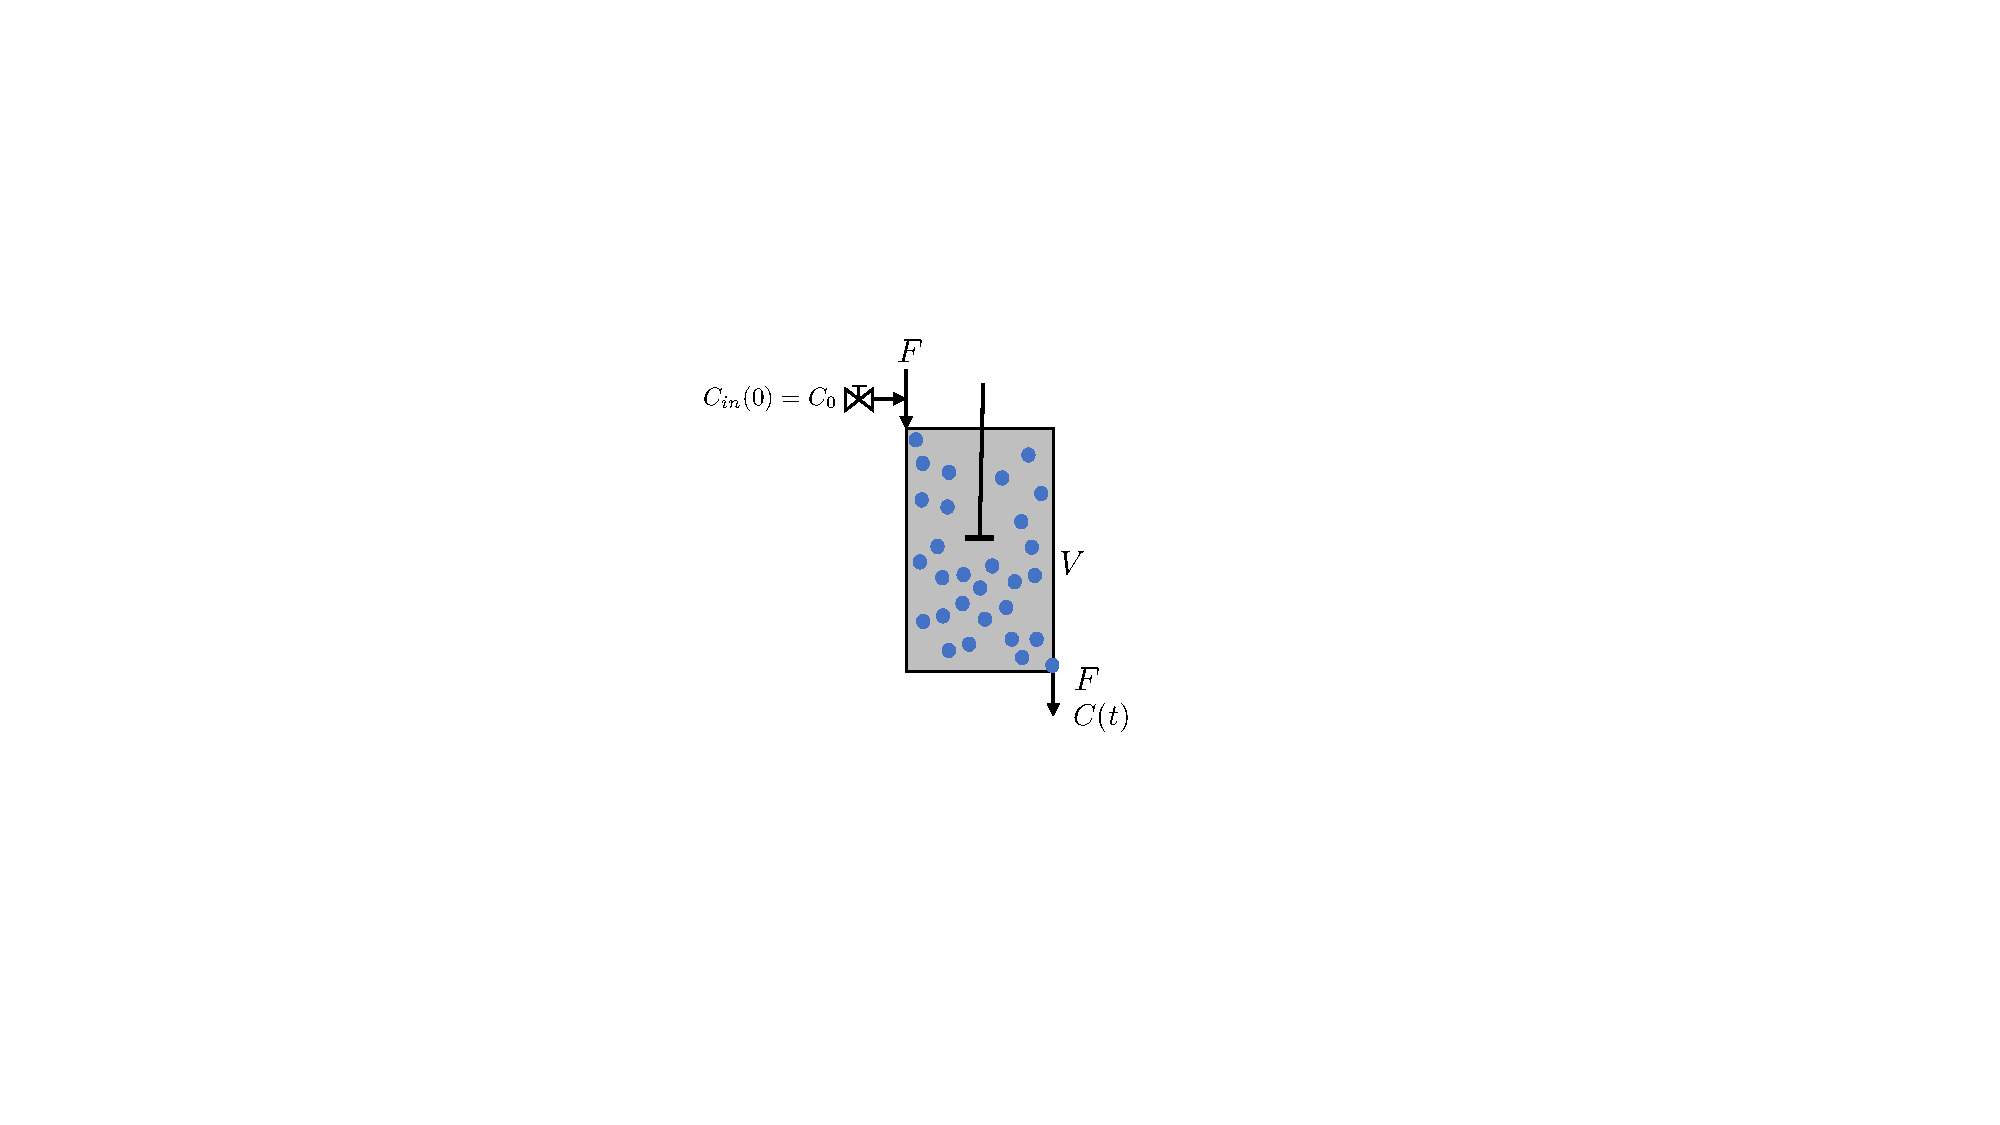
\includegraphics[width=0.3\textwidth]{figstats/particle_diagram}
\end{figure}
\pause
\begin{itemize}
\item A material balance for the system reveals that:
\begin{align}
f_T(t)=\frac{C(t)}{C_0}= \frac{1}{\tau}e^{-t/\tau}\;\; \textrm{with}\;\; \tau=V/F
\end{align}
\item Interpret $T$ as time required for particle to exit system (residence time)
\item Pdf $f_T(t)$ is interpreted as fraction of particles exiting at time $T=t$
\end{itemize}
\end{frame}
%------------------------------------------------

%------------------------------------------------
%
\begin{frame}{Example: Residence Time in Mixing System}

\begin{block}{}
\begin{align}
f_T(t)=\frac{C(t)}{C_0}= \frac{1}{\tau}e^{-t/\tau}\;\; \textrm{with}\;\; \tau=V/F
\end{align}
\end{block}
\begin{itemize}
\item Balance suggests that $T\sim\textrm{Exp}(\tau)$  
\item We thus have mean of residence time is $\mathbb{E}[T]=\tau=V/F$ and variance is $\mathbb{V}[T]=(V/F)^2$.  What is effect of $V$ and $F$? 
\item Fraction of particles that have exited up to time $t$ is $\mathbb{P}(T\leq t)=F_T(t)$. 
\item Note that $F_T(t)=\int_{0}^t(1/\tau)e^{-t/\tau}dt=(1-e^{-t/\tau})$ and thus $F(0)=0$ and $F(\infty)=1$.
\item Fraction of particles that are still in the system at time $t$  is $\mathbb{P}(T>t)=1-F_T(t)$. This function is known as the survival function. 
\end{itemize}
\end{frame}
%------------------------------------------------

%------------------------------------------------
%
\begin{frame}{Model of a Gamma RV}

The Gamma RV is a generalization of the exponential RV that has a pdf of the form:
\begin{block}{}
\begin{align*}
f_X(x)=\frac{1}{\beta^\alpha \Gamma(\alpha)}e^{-x/\beta}x^{\alpha-1},\; x\in \mathcal{D}_X=\{0\leq x\leq \infty\}.
\end{align*}
\end{block}
\begin{itemize}
\item The pdf has two hyperparameters $\alpha,\beta\in \mathbb{R}_+$
\item $\Gamma(\alpha)$ is the gamma function (for integer $\alpha\geq 1$ we have $\Gamma(\alpha)=(\alpha-1)!$). 
\item We express the fact that $X$ is a gamma RV as $X\sim \textrm{Gamma}(\alpha,\beta)$
\end{itemize}

\end{frame}
%------------------------------------------------

%------------------------------------------------
%
\begin{frame}{Model of a Gamma RV}

\begin{itemize}
\item The pdf tells us that one recovers an exponential RV when $\alpha=1$. 
\item The term $x^{\alpha-1}$ introduces a competing (opposite) effect for the exponential decay, giving rise to peak in the pdf. The location of this peak is $x^*=(\alpha-1)\beta$ and is the mode of the RV (point that maximizes $\mathbb{P}(X=x)$). 
\item The expected value and variance are $\mathbb{E}_X=\alpha\beta$ and $\mathbb{V}_X=\alpha\beta^2$ (i.e., the hyperparameters can be estimated from data by solving a set of two equations). 
\item In the context of time phenomena, this RV generalizes the exponential in that it models the amount of time that we have to wait until we observe the $\alpha$-th occurrence of an event. Consequently, $\alpha$=1 means the first event (as in the exponential RV). 
\item This RV has applications not only in temporal but also in spatial phenomena. For instance, it can be used to model the distance until we find the $\alpha$-th occurrence of certain type of atom in a molecule.  
\end{itemize}

\end{frame}
%------------------------------------------------


%------------------------------------------------
%
\begin{frame}{Model of an Gamma RV}
\begin{itemize}
\item Below at the pdfs and cdfs for $\textrm{Gamma}(\alpha,\beta)$ for different values of $\alpha,\beta$.
\end{itemize}
\begin{figure}[!htb]
    \centering
	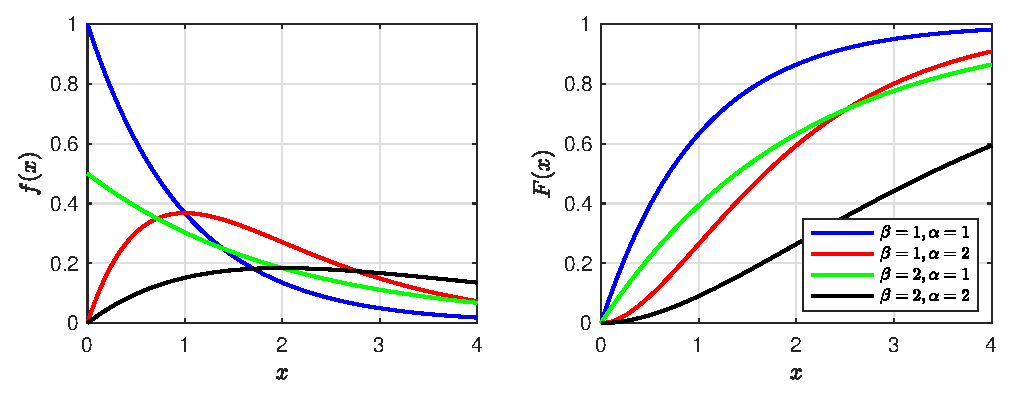
\includegraphics[width=0.8\textwidth]{figstats/Matlab/gamma}
\end{figure}
\begin{itemize}
\item Note same as exponential for $\alpha=1$.
\item Note emergence of peaks due to competing effects for $\alpha=2$. 
\end{itemize}
\end{frame}
%------------------------------------------------

%------------------------------------------------
%
\begin{frame}{Model of a Chi-Squared RV}

The Chi-Square RV has a pdf of the form:
\begin{block}{}
\begin{align*}
f_X(x)=\frac{1}{2^{r/2}\Gamma(r/2)}e^{-x/2}x^{r/2-1},\; x\in \mathcal{D}_X=\{0\leq x\leq \infty\}.
\end{align*}
\end{block}
\begin{itemize}
\item The pdf has only one hyperparameter $r\in \mathbb{Z}_+$ (a.k.a degrees of freedom).
\item We express the fact that $X$ is a gamma RV as $X\sim \chi^2(r)$
\item Note that this is a Gamma RV with $\beta=2$ and $\alpha=r/2$ (for a positive integer $r$). 
\item The expected value and variance can be derived from those of the Gamma RV.  
\item A crucial property of a Chi-Squared RV is that it is related to the standard normal RV. In particular, one can show that: 
\begin{align*}
\sum_{i=1}^rX_i^2\sim \chi^2(r)
\end{align*}
if $X_i\sim \mathcal{N}(0,1)$. This property will be useful later on. 
\item From relationship with $\mathcal{N}(0,1)$ we can show that $\mathbb{Q}(1-\alpha)$ of $\chi^2(1)$ is equal to $\mathbb{Q}(1-\alpha/2)^2$ of $\mathcal{N}(0,1)$. This is because $\mathbb{P}(-z\leq Z\leq z)=\mathbb{P}(Z^2\leq z)$.  
\end{itemize}

\end{frame}
%------------------------------------------------

%------------------------------------------------
%
\begin{frame}{Model of an Chi-Squared RV}
\begin{itemize}
\item Compare quantile functions of $\mathbb{Q}(1-\alpha)$ of $\chi^2(1)$ and $\mathbb{Q}(1-\alpha/2)^2$ of $\mathcal{N}(0,1)$.
\end{itemize}
\begin{figure}[!htb]
    \centering
	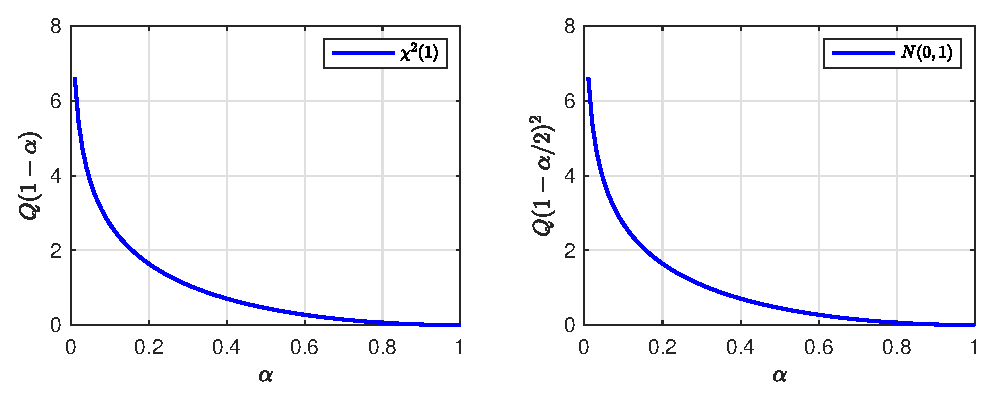
\includegraphics[width=0.8\textwidth]{figstats/Matlab/quantiles_norm_chi2}
\end{figure}
\end{frame}
%------------------------------------------------


%------------------------------------------------
%
\begin{frame}{Model of a Weibull RV}

The Weibull RV is a generalization of the exponential RV that has a pdf:
\begin{block}{}
\begin{align*}
f_X(x)=\frac{\xi}{\beta}\left(\frac{x}{\beta}\right)^{\xi-1}\exp\left[{-\left(\frac{x}{\beta}\right)^\xi}\right],\; x\in \mathcal{D}_X=\{0\leq x\leq \infty\}.
\end{align*}
\end{block}
\begin{itemize}
\item The pdf has two hyperparameters $\xi,\beta\in \mathbb{R}_+$ (a.k.a scale and shape).
\item We express the fact that $X$ is a gamma RV as $X\sim \textrm{Weibull}(\xi,\beta)$.
\item Note that one recovers an exponential RV when $\xi=1$. 
\item The expected value and variance are $\mathbb{E}_X=\beta\Gamma(1+1/\xi)$ and $\mathbb{V}_X=\beta^2\left(\Gamma(1+2/\xi)+\Gamma(1+1/\xi)^2\right)$. The dependence on the gamma function makes it difficult to estimate $\xi,\beta$ from these relationships. 
\item cdf has a nice form $F_X(x)=1-e^{(-x/\beta)^\xi}$ ($\xi,\beta$ are often inferred from the cdf). Note that $\mathbb{P}(X\leq \beta)=0.632$ for any $\xi$. 
\item Weibull RV is the {\em de facto} model used in failure analysis and was discovered by Fischer and Tippett. 
\item Turns out that, as in the case of the Gaussian RV, many phenomena have the Weibull RV as a limiting case (we will show this later). 
\end{itemize}

\end{frame}
%------------------------------------------------

%------------------------------------------------
%
\begin{frame}{Model of Weibull RV}
\begin{itemize}
\item Below at the pdfs and cdfs for $\textrm{Weibull}(\beta,\xi)$ for different values of $\beta,\xi$.
\end{itemize}
\begin{figure}[!htb]
    \centering
	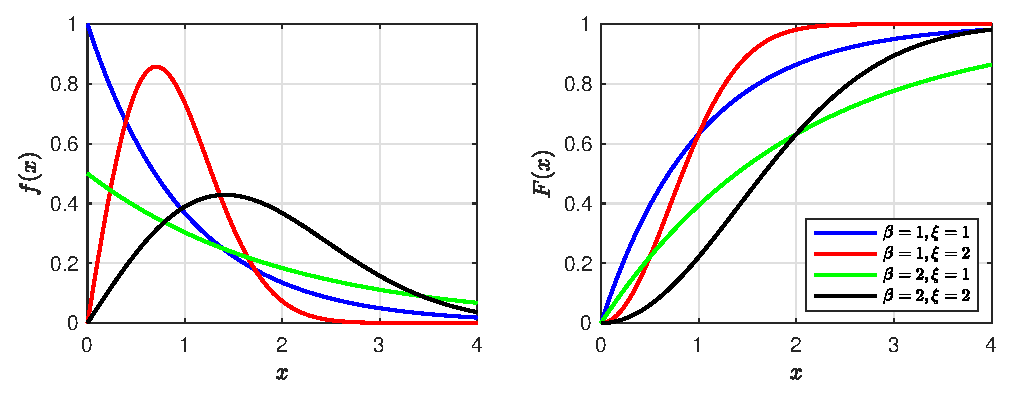
\includegraphics[width=0.8\textwidth]{figstats/Matlab/weibull}
\end{figure}
\begin{itemize}
\item Note same as exponential for $\xi=1$.
\item Note emergence of peaks due to competing effects for $\xi=2$. 
\item Note $\mathbb{P}(X\leq \beta)=0.632$ for any $\xi$ (this differentiates it from Gamma RV).
\end{itemize}
\end{frame}
%------------------------------------------------

%------------------------------------------------
%
\begin{frame}{Families of Random Variables}
\begin{itemize}

\item The exponential, Gamma, Chi-Squared, and Weibull RVs are interrelated. In fact, these are captured by the generalized gamma model with pdf:
\begin{block}{}
\begin{align*}
F_X(x)=\frac{1}{\beta^{\alpha\xi}\Gamma(\alpha)}\exp\left[-\left(\frac{x-\delta}{\beta}\right)^\xi\right]\xi(x-\delta)^{\alpha\xi-1},\quad x\in \mathcal{D}_X=\{0\leq x\leq \infty\}.
\end{align*}
\end{block}
\item These RVs are known as the Gamma family. 
\item There are three major families of continuous RVs: 
\begin{itemize}
\item Gaussian family (includes Gaussian, LogNormal, and Raylegh)
\item Gamma family (includes exponential, Gamma, Chi-Squared, and Weibull)
\item Ratio family (includes Cauchy, Uniform, Beta, Fisher, Student)
\end{itemize}

\item There is one family for discrete RVs, which includes Uniform (discrete), Bernoulli, Bionomial, and Poisson.

\item Each family models different type of phenomena and there exist relationships between RVs within families and across families. 

\end{itemize}
A detailed discussion of the modeling properties of RVs is beyond our scope. Here, we have only discussed the RVs that will be relevant in our subsequent discussion. 

\end{frame}
%------------------------------------------------

%------------------------------------------------
%
\begin{frame}{Families of Random Variables}

\begin{figure}[!htb]
    \centering
	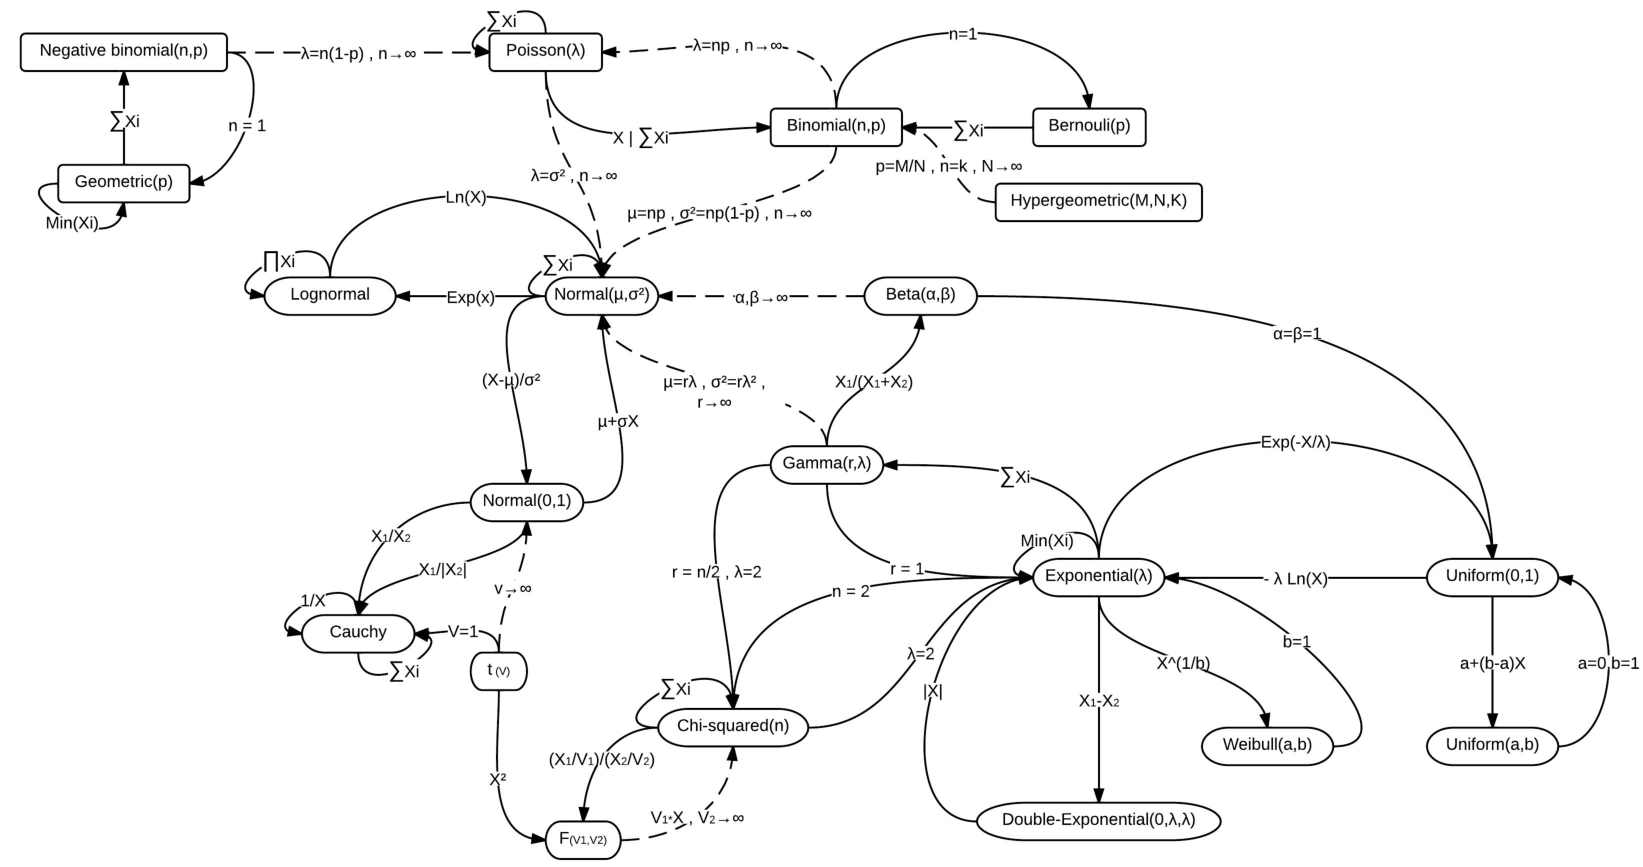
\includegraphics[width=\textwidth]{figstats/familiesRV}
\end{figure}

\end{frame}
%------------------------------------------------


%------------------------------------------------
%
\begin{frame}{Estimation Techniques}


\begin{itemize}
\item Now that we have a basic idea of the types of RV models available we proceed to develop procedures to estimate an RV model from available data. 

\item We will  define an RV model in terms of its $f_X(x|\theta)$ (or $F_X(x|\theta)$), where $\theta$ are the hyperparameters. 

\item By estimating an RV model we mean that we seek to find $\theta$ that best fits the data.

\end{itemize}

\begin{block}{}
We will explore a couple of estimation methods:
\begin{itemize}
\item Point Estimation (Method of Moments and Least-Squares Method)

\item Maximum Likelihood Estimation
\end{itemize}
\end{block}

\begin{itemize}
\item Our first step will be to explore our data and postulate a specific RV model (e.g., Gaussian or Exponential) based on any patterns exposed by the data. 
\item Our second step would be to tune $\theta$ for the given postulated RV model to see if this fits the data satisfactorily. If the fit is not adequate, we postulate another model.
\end{itemize}

\end{frame}
%------------------------------------------------

%%------------------------------------------------
%%
\begin{frame}{Method of Moments}

\begin{itemize}
\item Recall the moments of $X$ (with pdf $f_X(x|\theta)$ and hyperprameters $\theta$) are given by:
\begin{align*}
m_k(\theta):=\mathbb{E}[(X-\mathbb{E}[X])^k], \qquad k=1,2,...,N
\end{align*}
\item Here, we highlight the dependence of the moments on the hyperparameters $\theta$. 

\item Method of moments uses data $x_\omega,\; \omega \in \mathcal{S}$ to obtain sample approximations: 
\begin{align*}
M_k&=\frac{1}{S}\sum_{\omega\in \mathcal{S}}(x_\omega-m)^k, \; k=1,2,...,N
\end{align*}
where $m=\frac{1}{S}\sum_{\omega\in \mathcal{S}}x_\omega$ is the sample mean.

\end{itemize}

\end{frame}
%------------------------------------------------


%%------------------------------------------------
%%
\begin{frame}{Method of Moments}

\begin{itemize}

\item Our objective is to find the hyperparameters $\theta$ that solve the matching equations:
\begin{align*}
m_k(\theta)=M_k,\; k=1,2,...,N
\end{align*}
\item In other words, we want to find $\theta$ that matches model and data moments. 

\item A solution to the equations can also be found by solving the minimization problem:
\begin{align*}
\min_\theta \frac{1}{2}\sum_{k=1}^N(m_k(\theta)-M_k)^2.
\end{align*}
This problem is known as a least-squares minimization problem (seeks to minimize the discrepancy between the model and data moments). 

\item Least-squares is preferred when the matching equations do not have a solution. In this case, the minimization problem finds $\theta$ that is most compatible with the data.  

\end{itemize}

\end{frame}
%------------------------------------------------


%------------------------------------------------
%
\begin{frame}{Example: Method of Moments}

We illustrate how to estimate $\theta=(\mu,\sigma^2)$ using moment matching for $\mathcal{N}(0,1)$.
\begin{itemize}
\item We are given observations $x_\omega,\; \omega \in \mathcal{S}$.
\item Sample mean is $\hat{E}_X=\frac{1}{S}\sum_{s\in\mathcal{S}}x_\omega$ and variance $\hat{V}_X=\frac{1}{S}\sum_{s\in\mathcal{S}}(x_\omega-\hat{\mathbb{E}}_X)^2$. 
\item We have that $m_1(\theta)=\mathbb{E}[X-\mathbb{E}_X]=\mathbb{E}_X-\mu=0$ and thus we estimate $\mu=\hat{\mathbb{E}}_X$.
\item We have that $m_2(\theta)=\mathbb{V}_X=\sigma^2$ and thus we estimate $\sigma^2=\hat{\mathbb{V}}_X$
\end{itemize}
Now consider we wish to estimate $\theta=(\xi,\beta)$ using moment matching for $\textrm{Weibull}(\xi,\beta)$. 
\begin{itemize}
\item We are given observations $x_\omega,\; \omega \in \mathcal{S}$.
\item Sample mean is $\hat{E}_X=\frac{1}{S}\sum_{s\in\mathcal{S}}x_\omega$ and variance $\hat{V}_X=\frac{1}{S}\sum_{s\in\mathcal{S}}(x_\omega-\hat{\mathbb{E}}_X)^2$. 
\item We find $\beta,\xi$ that match $m_1(\theta)$ and $m_2(\theta)$ by solving the nonlinear equations:
\begin{align*}
\hat{\mathbb{E}}_X&=\beta\Gamma(1+1/\xi)\\
\hat{\mathbb{V}}_X&=\beta^2\left(\Gamma(1+2/\xi)+\Gamma(1+1/\xi)^2\right)
\end{align*}
\item This is computationally challenging due to $\Gamma$ function.  Is there another way?
\end{itemize}
\end{frame}
%------------------------------------------------

%------------------------------------------------
%
\begin{frame}{Least-Squares Method}

\begin{itemize}

\item Functional form of moments $m_k(\theta)$ might be too complex for some RVs (e.g., Weibull).

\item In such cases, we can use $F_X(t|\theta)$ to find the hyperparameters. For example, for Weibull we have $F_X(t|\theta)=(1-e^{-(t/\beta)^\xi})$ with $\theta=(\xi,\beta)$. 

\item In least-squares method, we find $\theta$ that best matches the empirical cdf (obtained from data $x_\omega,\; \omega \in \mathcal{S}$). 

\item Here, we propose a set of threshold values $t_k, k=1,2,...,N$ and compute:
\begin{align*}
\hat{F}_k=\frac{1}{S}\sum_{\omega \in \mathcal{S}}\mathbf{1}[x_\omega\leq t_k],\; k=1,2,...,N
\end{align*}

\item  We use these approximations to solve the least-squares minimization problem:
\begin{align*}
\min_\theta \frac{1}{2}\sum_{k=1}^N(F_X(t_k|\theta)-\hat{F}_k)^2
\end{align*}
\item When  cdf has exponential form, it is convenient to use log transformations such as:
 \begin{align*}
\min_\theta \frac{1}{2}\sum_{k=1}^N(\log F_X(t_k|\theta)-\log \hat{F}_k)^2
\end{align*}
\item Least-squares method is general and can be used to match other statistics of the RV available such as empirical quantiles, and empirical pdfs. 

\end{itemize}

\end{frame}
%------------------------------------------------


%------------------------------------------------
%
\begin{frame}{Example: Weibull using Least-Squares}

Consider we wish to estimate $\theta=(\xi,\beta)$ using least-squares for $\textrm{Weibull}(\xi,\beta)$. 
\begin{itemize}
\item We are given observations $x_\omega,\; \omega \in \mathcal{S}$ and obtain empirical cdfs $\hat{F}(t_k)$ for given $t_k,\, k=1,...,N$. 
\item Recall cdf of Weibull is $F_X(t|\theta)=(1-e^{-(t/\beta)^\xi})$ and notice that:
\begin{align*}
\log(1-F_X(t|\theta))=-(t/\beta)^\xi
\end{align*}
Moreover, note that:
\begin{align*}
\log(-\log(1-F_X(t|\theta)))= \xi \log t-\xi \log \beta
\end{align*}
\item We have $\log t=a\log(-\log(1-F_X(t|\theta)))+b$ with $a=1/xi$ and $b=\log\beta$. 
\item We want to find $a,b$ that best match equations $\log t_k=a\cdot \log(-\log(1-\hat{F}(t_k))+b$. This is done by solving:
\begin{align*}
\min_{a,b}\; \sum_{k=1}^N\left (y_k-(a\cdot x_k+b)\right)^2
\end{align*}
where $x_k=\log(-\log(1-\hat{F}(t_k))$ and $y_k=\log t_k$. 
\item This is a simple linear optimization problem. We will see later one how to solve this. 
\end{itemize}


\end{frame}
%------------------------------------------------

%------------------------------------------------
%
\begin{frame}{Example: Weibull using Least-Squares}

\begin{figure}[!htb]
    \centering
	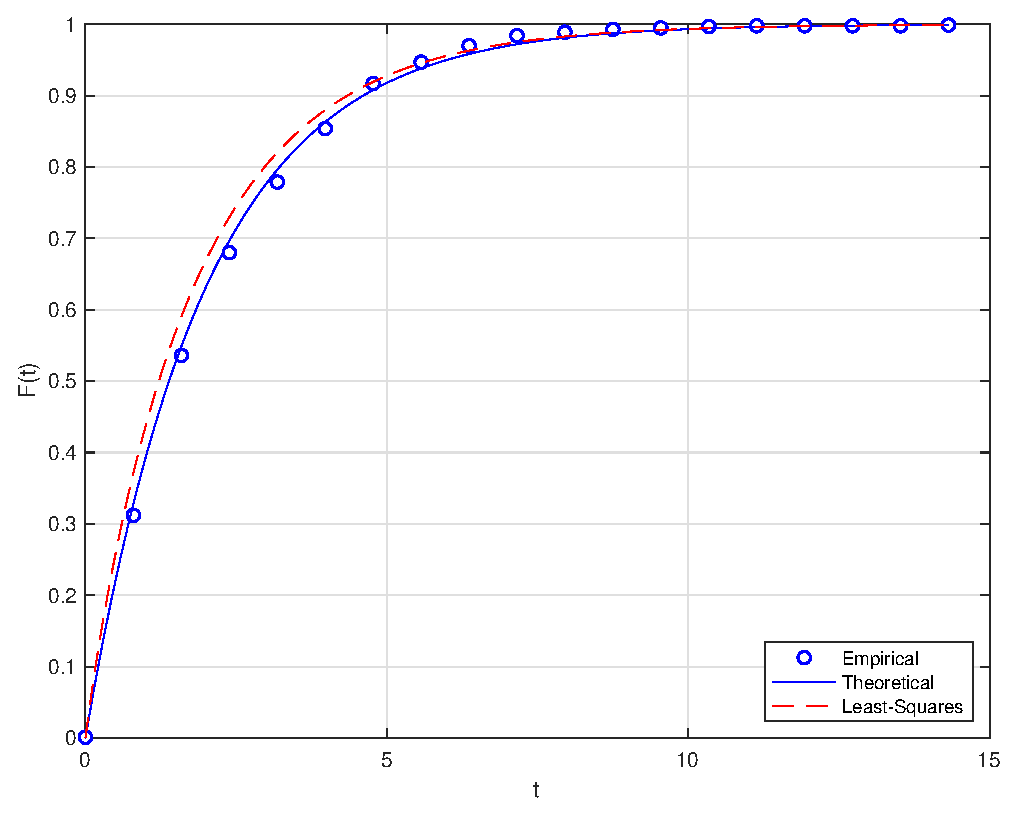
\includegraphics[width=0.8\textwidth]{figstats/Matlab/lsfit_weibull}
\end{figure}

\end{frame}
%------------------------------------------------

%------------------------------------------------
%
\begin{frame}{Maximum Likelihood Method}

The maximum likelihood estimation (MLE) method proceeds as follows:

\begin{itemize}
\item Assume we have observations $x_\omega,\, \omega \in \mathcal{S}$ (selected at random).
\item We postulate $f_X(x|\theta)$ for the RV $X$ and recall that $f(x_\omega|\theta)$ is the probability (likelihood) that $X$ takes the value of observation $x_\omega$.  

\item Consequently, we find hyperparameters $\theta$ that maximize {\em joint} probability that $X$ takes observations $x_\omega,\,\omega \in \mathcal{S}$. This is done by solving the maximization problem:
\begin{align*}
\max_\theta\; L(\theta)=\prod_{\omega \in \mathcal{S}}f(x_\omega|\theta).
\end{align*}
Here, $L(\theta)$ is known as the likelihood function. 

\item It is often convenient to solve the equivalent problem:
\begin{align*}
\max_\theta\; \log L(\theta)=\sum_{\omega \in \mathcal{S}}\log f(x_\omega|\theta).
\end{align*}
This problem can be solved by hand when the pdf is simple but requires numerical techniques when complex. 
\item We will soon discuss what ``random observations" and ``joint probability" mean. 
\end{itemize}

\end{frame}
%------------------------------------------------


%------------------------------------------------
%
\begin{frame}{Example: Maximum Likelihood for Exponential RV}

\begin{itemize}
\item Want to estimate $\beta$ for $\textrm{Exp}(\beta)$ using observations $x\_omega$. 
\item Pdf of the exponential is $f(x|\beta)=\frac{1}{\beta}e^{-x/\beta}$ and thus likelihood function:
\begin{align*}
L(\beta)&=\left(frac{1}{\beta}e^{-x_1/\beta}\right)\left(\frac{1}{\beta}e^{-x_2/beta}\right)\cdots\left(\frac{1}{\beta}e^{-x_S/\beta}\right)\\
&=\frac{1}{\beta^S}\exp \left(-\frac{1}{\beta}\sum_{\omega=1}^Sx_\omega\right).
\end{align*}
\item We find $\beta$ that maximizes log likelihood $\log L(\beta)$:
\begin{align*}
\max_{\beta}\; \log L(\beta)=-S\log \beta -\frac{1}{\beta}\sum_{\omega=1}^Sx_\omega
\end{align*}
\item The solution of this problem indicates that $\hat{\beta}=\frac{1}{S}\sum_{\omega=1}^Sx_\omega$.
\item Best estimate $\hat{\beta}$ is sample mean (which makes sense because $\mathbb{E}[X]=\beta$). 
\end{itemize}


\end{frame}
%------------------------------------------------

%------------------------------------------------
%
\begin{frame}{Example: Maximum Likelihood for Exponential RV}

\begin{itemize}
\item Here we present a plot for $\log L(\beta)$ using data $x_\omega$ generated from $\textrm{Exp}(2)$. 
\item Value of $\beta$ that maximizes $\log L(\beta)$ ($\hat{\beta}$) coincides with true value $\beta=2$. 
\end{itemize}
\begin{figure}[!htb]
    \centering
	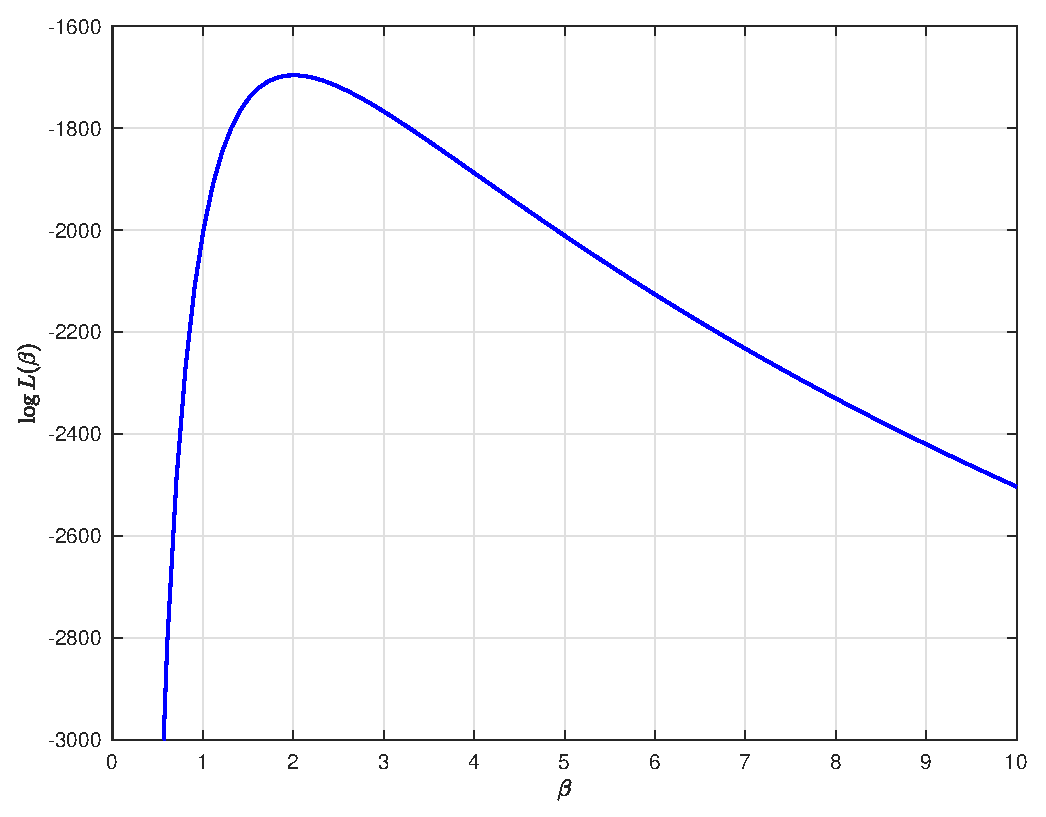
\includegraphics[width=0.7\textwidth]{figstats/Matlab/loglike_exp}
\end{figure}

\end{frame}
%------------------------------------------------


%------------------------------------------------
%
\begin{frame}{Sampling and Asymptotic Properties}

So far, we have assumed that we have data $x_\omega,\; \omega \in \mathcal{S}$ but we have not discussed yet how this is being collected and generated.  Moreover, we want to know how our empirical approximations behave as we keep accumulating data.  

\begin{itemize}
\item The data sample sequence $x_\omega \in \mathcal{S}$ is a set of observations of $X$ collected from a statistical population $\Omega$ by a defined procedure; i.e., sampling is a data collection procedure. 

\item A data sample sequence $x_\omega \in \mathcal{S}$ is called random if each sample $x_\omega$ is drawn from the same underlying pdf $f_X(x)$ and if it is drawn independently from the others. In other words, the samples are independent and identically distributed (i.i.d).

\item If a sample $x_\omega$ is selected at random, the sample itself is an RV. Consequently, sometimes we denote the data sample sequence as a sequence of RVs $X_\omega \in \mathcal{S}$.  

\end{itemize}

\end{frame}
%------------------------------------------------

%------------------------------------------------
%
\begin{frame}{Sampling and Asymptotic Properties}

\begin{itemize}

\item Random sample $X_\omega$ has same probability $1/S$ of being selected and is {\em unbiased}. 

\item The lack of bias indicates that $\mathbb{E}[X_\omega]=\mathbb{E}[X]$ (drawing sample many times and averaging the results gives same expected value of the actual RV $X$). 

\item Random samples can be used to construct approximation techniques with rather striking asymptotic properties, as we will show next.  

\item Collecting data at random is not as easy as it sounds, one must ensure that there is no bias in selecting a sample (i.e., there is no hidden mechanism).  As humans, it is strikingly difficult to pick something randomly. 

\end{itemize}

\end{frame}
%------------------------------------------------

%------------------------------------------------
%
\begin{frame}{Sampling and Asymptotic Properties}
\begin{itemize}
\item Below we show a random and nonrandom sample sequence for $\mathcal{N}(0,1)$ and their corresponding long-term  averages. 
\item For nonrandom, we select a particular element of the sample (this introduces a bias). 
\end{itemize}
\begin{figure}[!htb]
    \centering
	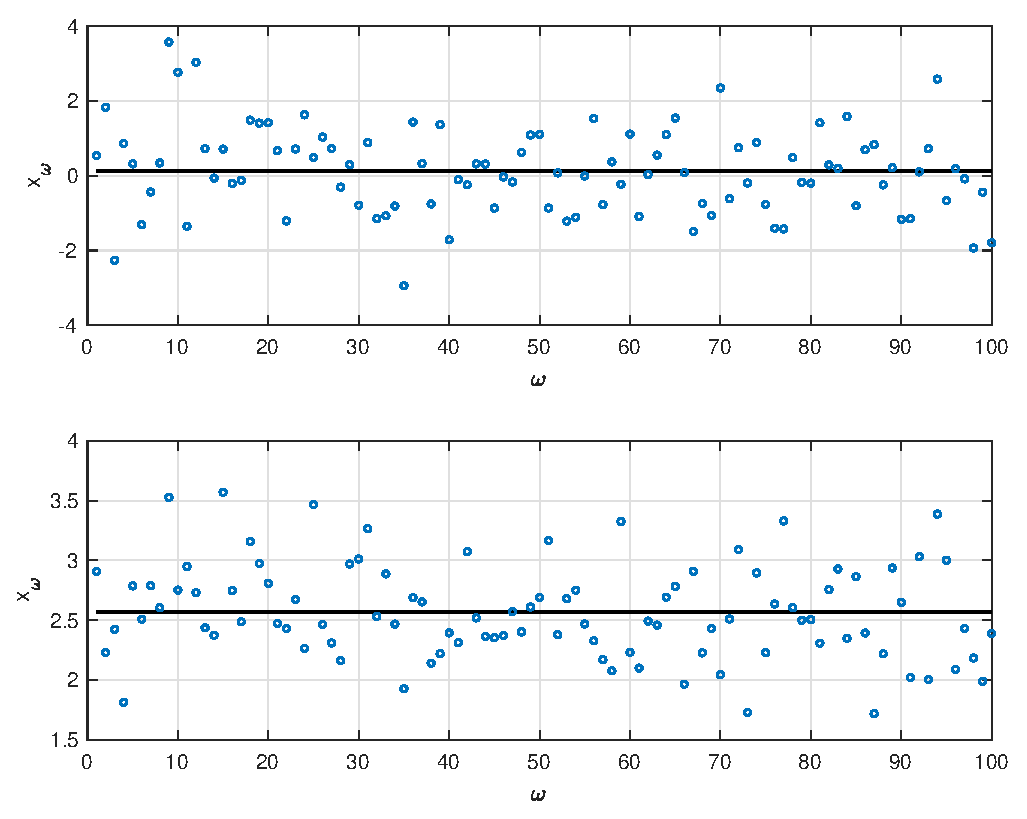
\includegraphics[width=0.6\textwidth]{figstats/Matlab/random_sample}
\end{figure}

\end{frame}
%------------------------------------------------

%------------------------------------------------
%
\begin{frame}{Monte Carlo Approximations}

{\em Monte Carlo} (MC) is a set of computational techniques that use {\em random samples} to infer properties of $X$ and derived quantities (e.g., summarizing statistics).  For example, we can use the random sample $x_\omega \in \mathcal{S}$ to compute the sample approximations:
\begin{block}{}
\begin{itemize}
\item Expectation of $X$: $\hat{E}_X^S:=\frac{1}{S}\sum_{\omega \in \mathcal{S}}x_\omega\approx \mathbb{E}[X]$
\item Variance of $X$: $\hat{V}_X^S:=\frac{1}{S}\sum_{\omega \in \mathcal{S}}(x_\omega-\hat{E}_X^S)^2\approx \mathbb{V}[X]$
\item CDF of $X$: $\hat{F}_X^S(x):=\frac{1}{S}\sum_{\omega 
\in \mathcal{S}}\mathbf{1}[x_\omega \leq x]\approx F_X(x)=\mathbb{E}[{\mathbf{1}[X \leq x]}]$
\item Expectation of system $\hat{E}_\varphi^S:=\frac{1}{S}\sum_{\omega 
\in \mathcal{S}}\varphi(x_\omega,u)\approx \mathbb{E}[{\varphi(X,u)}]$. 
\end{itemize}
\end{block}
Natural questions that emerge here are: 
\begin{block}{}
\begin{itemize}
\item Do the approximations become exact as $S\to \infty$?
\item How accurate are these approximations for finite $S$?
\end{itemize}
\end{block}
\begin{itemize}
\item Most approximations use an expectation function and we thus restrict our discussion to the behavior of the approximation $\hat{E}_X^S$. 
\item There are approximation techniques that use systematic (biased) sampling methods (data is not collected at random). 
\end{itemize}
\end{frame}
%------------------------------------------------

%------------------------------------------------
%
\begin{frame}{Law of Large Numbers}

Lets first assess the quality of the MC approximation as $S\to \infty$. 
\begin{itemize}
\item Consider a random sample sequence $X_1,X_2,...,X_S$ for RV $X$. Since samples are identically distributed, they have same underlying pdf with expected value $\mathbb{E}[X]$. 
\item This implies that $\mathbb{E}[X_1]=\mathbb{E}[X_2]=\cdots=\mathbb{E}[X_S]=\mathbb{E}[X]$. 
\item Consider the MC approximation of $\mathbb{E}[X]$:
\begin{align*}
\hat{\mathbb{E}}_X^S=\frac{1}{S}\sum_{\omega \in \mathcal{S}}X_\omega
\end{align*}
\end{itemize}
\begin{block}{}
The law of large numbers (LLN) states that:
\begin{align*}
\lim_{S\to \infty}\hat{\mathbb{E}}_X^S=\mathbb{E}[X]
\end{align*}
\end{block}
\begin{itemize}
\item The LLN is a fundamental result in statistics and is important because it guarantees {\em stable long-run} behavior of random variables.  

\item In other words, if the process is truly random, samples fluctuate around $\mathbb{E}[X]$ and average out.  Conversely, if there is a systematic bias, the fluctuations will accumulate and the process will drift. 

\item The LLN implies that Monte Carlo approximations become asymptotically exact as $S\to \infty$. Importantly, the result holds for any random variable (e.g., discrete, continuous, univariate, multivariate). 
\end{itemize}

\end{frame}
%------------------------------------------------

%------------------------------------------------
%
\begin{frame}{Example: Monte Carlo Approximations}

\begin{itemize}
\item Consider random samples $x_\omega,\; \omega \in \mathcal{S}$ obtained from $X\sim \textrm{Weibull}(2,1)$
\item MC approximations for $\mathbb{E}[X],\mathbb{E}[\log(X)]$ and $\mathbb{V}[\exp(X)+X^2]$  for different $S$.
\end{itemize}
\begin{figure}[!htb]
    \centering
	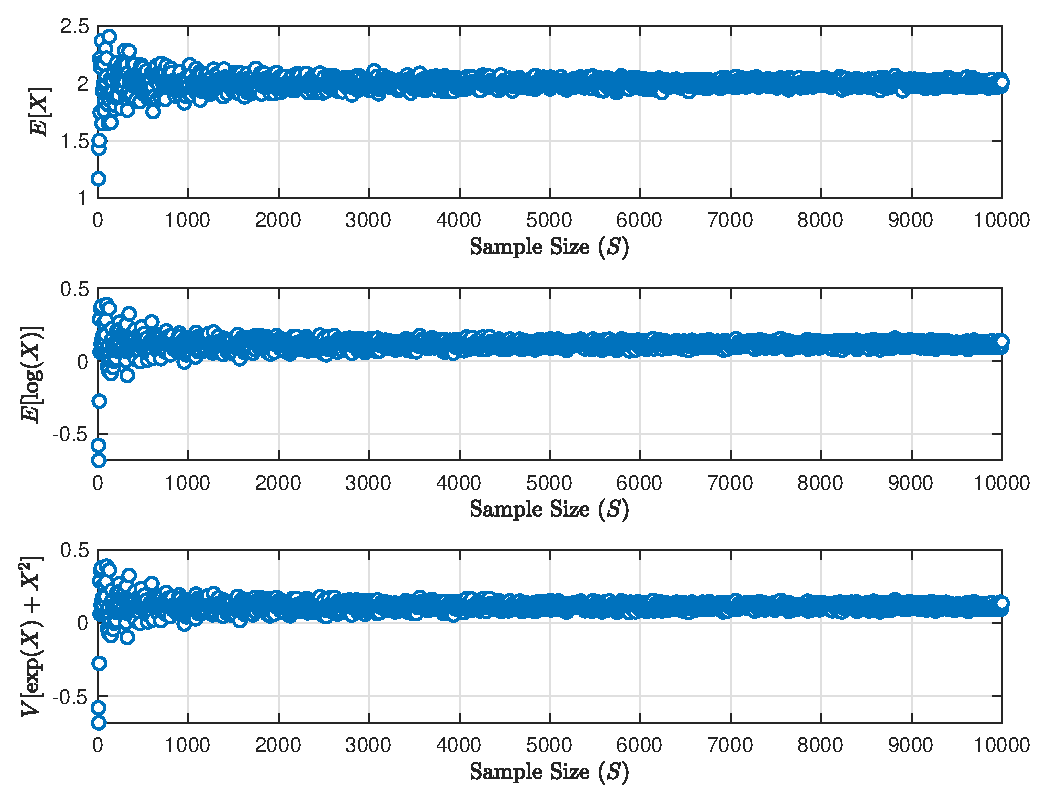
\includegraphics[width=0.6\textwidth]{figstats/Matlab/convergence_mc}
\end{figure}


\end{frame}
%------------------------------------------------

%------------------------------------------------
%
\begin{frame}{Central Limit Theorem}

lets turn our attention to the issue of assessing quality of the MC approximation for finite sample size $S$. 
\begin{itemize}
\item This can be addressed by using a powerful result in statistics known as the central limit theorem (CLT). 
\item Consider that the random sample sequence $X_1,X_2,...,X_S$ is i.i.d and has {\em known} expected value $e=\mathbb{E}[X]$ and variance $v^2=\mathbb{V}[X]$. 

\item We know that $X_\omega$ are RVs and so is $\hat{\mathbb{E}}_X^S$. 
\end{itemize}

The CLT will answer the following questions:
\begin{block}{}
\begin{itemize}
\item What is the distribution of $\hat{\mathbb{E}}_X^S$? If we know it, we can say something about how much variability the MC  approximation has. 

\item What is the distribution of $\hat{\mathbb{E}}_X^S$ as $S\to \infty$? 
\end{itemize}
\end{block}

\end{frame}
%------------------------------------------------

%------------------------------------------------
%
\begin{frame}{Central Limit Theorem}

\begin{block}{}
The CLT states that:
\begin{align*}
\lim_{S\to \infty}\hat{\mathbb{E}}_X^S\sim \mathcal{N}(e,v/\sqrt{S})
\end{align*}
\end{block}

This result is one of the most surprising and useful results in statistics. Let's explain why:

\begin{itemize}

\item CLT says that, {\em regardless} of the underlying nature of $X$ (e.g., Uniform, Weibull, Exponential), its sample average approximation $\hat{\mathbb{E}}_X^S$ will {\em always} become a Gaussian RV as $S$ increases.  

\item CLT also says that the variance of the Gaussian $\hat{\mathbb{E}}_X^S\sim \mathcal{N}(e,v/\sqrt{S})$ shrinks with $S$. In other words, $\hat{\mathbb{E}}_X^S$ becomes more certain as $S$ increases.

\item Implication is that, since we have a cdf and pdf for $\hat{\mathbb{E}}_X^S$, we can compute all quantities of interest for it (e.g., confidence regions):
\begin{align*}
\mathbb{P}\left(e-z_{1-\alpha/2}v/\sqrt{S}\leq \hat{\mathbb{E}}_X^S\leq e+z_{1-\alpha/2}v/\sqrt{S}\right)=1-\alpha.
\end{align*}
Consequently, for given $S$, we can know how confident we are that the approximation $\hat{\mathbb{E}}_X^S$ is in a region.  

\end{itemize}


\end{frame}
%------------------------------------------------

%------------------------------------------------
%
\begin{frame}{Example: Central Limit Theorem}

\begin{itemize}
\item We a sample $X_1,X_2...,,X_S$ obtained from $X\sim \textrm{Weibull}(2,1)$.
\item Want distribution of $\bar{X}=\frac{1}{S}\sum_{\omega=1}X_\omega$ for different values of $S$.
\item Below we show pdf of $\textrm{Weibull}(2,1)$ and of $\bar{X}$ for $S=10,100,1000$.
\end{itemize}
\begin{figure}[!htb]
    \centering
	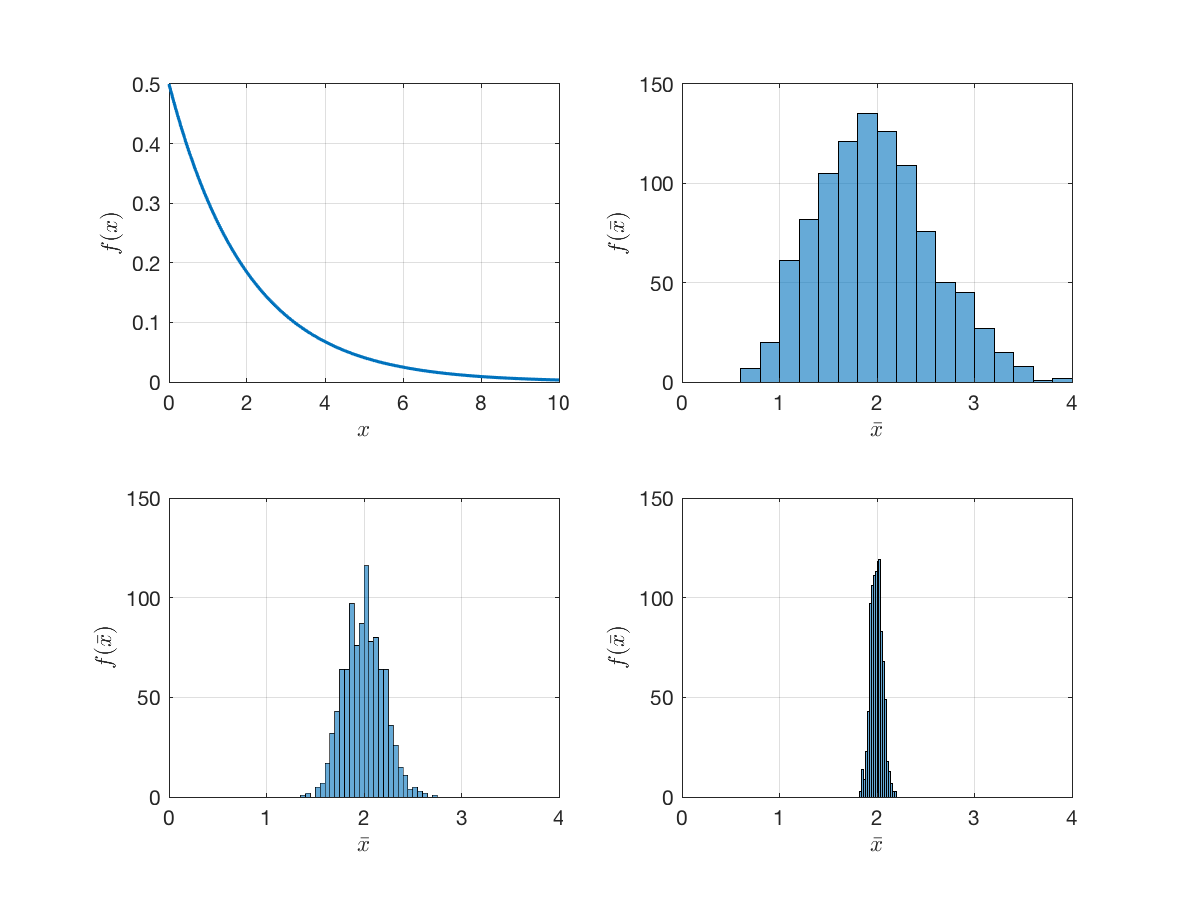
\includegraphics[width=0.7\textwidth]{figstats/Matlab/clt_weibull}
\end{figure}
\end{frame}
%------------------------------------------------


%------------------------------------------------
%
\begin{frame}{Extreme Value Distribution}

\begin{itemize}
\item In CLT we are interested in {\em sample average} $\hat{\mathbb{E}}_X^S=\frac{1}{S}\sum_{\omega\in \mathcal{S}}X_\omega$. 

\item But what if we are interested in a different statistic? For instance, the {\em sample max}:
\begin{align*}
X_{max}^S=\max\{X_1,X_2,\cdots, X_S\}
\end{align*}

\item There exists a result (analogous to CLT) that characterizes pdf of $X_{max}^S$ as $S\to \infty$.  The result is known as the extreme value theorem (EVT).

\item Consider, as before, a random sample sequence $X_1,X_2,...,X_S$ for RV $X$. 

\end{itemize}

\begin{block}{}
The EVT states that:
\begin{align*}
\lim_{S\to \infty}X_{max}^S\sim \textrm{GEV}(a,b,c)
\end{align*}
\end{block}
where $GEV(a,b,c)$ is the generalized extreme value RV with hyperparameters $a,b,c$. 

\end{frame}
%------------------------------------------------

%------------------------------------------------
%
\begin{frame}{Extreme Value Distribution}

The generalized extreme value RV has a pdf of the form:
\begin{block}{}
\begin{align*}
f(s;\xi) = \begin{cases}(1+c s)^{(-1/c)-1} \exp(-(1+c s)^{-1/c}) & c\neq0 \\
\exp(-s) \exp(-\exp(-s)) & c = 0\end{cases}
\end{align*}
and a cdf of the form:
\begin{align*}
F_X(x)= \begin{cases}\exp(-(1+c s)^{-1/c}) & c\neq0 \\ \exp(-\exp(-s)) & c = 0\end{cases}
\end{align*}
where $s=(x-a)/b$ is a standard variable. 
\end{block}
\begin{itemize}
\item GEV RV is a generalization that includes Weibull (for $c<0$), Frechet (for $c>0$), and Gumbel (for $c=0$) RVs. 


\item GEV RV is widely used in failure analysis because max operator characterizes peak (extreme) events. 

\item As with CLT,  EVT does not depend on the underlying nature of $X$. 

\end{itemize}


\end{frame}
%------------------------------------------------

%------------------------------------------------
%
\begin{frame}{Example: Extreme Value Theorem}

\begin{itemize}
\item We a sample $X_1,X_2...,,X_S$ obtained from $X\sim \mathcal{N}(2,1)$.
\item Want distribution of $X_{max}=\max\{X_1,X_2,\cdots, X_S\}$ for different values of $S$.
\item Below we show pdf of $X\sim \mathcal{N}(2,1)$. and of $\bar{X}$ for $S=10,100,1000$.
\end{itemize}
\begin{figure}[!htb]
    \centering
	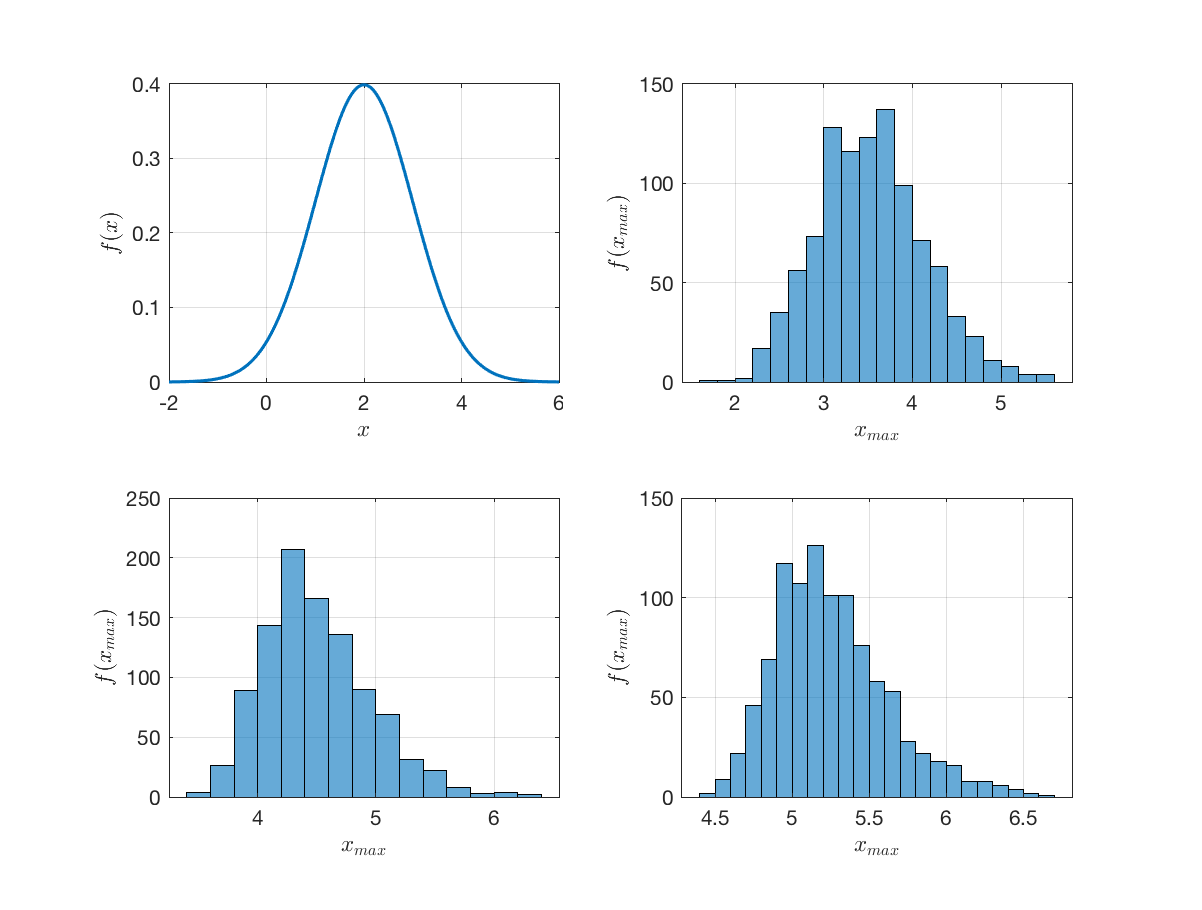
\includegraphics[width=0.7\textwidth]{figstats/Matlab/evt_weibull}
\end{figure}

\end{frame}
%------------------------------------------------

%------------------------------------------------
%
\begin{frame}{Multivariate Statistics}

\begin{itemize}
\item So far, we have assumed that the RV $X$ is univariate and thus has observations that are scalar values ($x_\omega \in \mathbb{R}$).  

\item We have also informally mentioned the concept of independent and joint RVs in the context of estimation and sampling.  What do these mean?

\item Consider a multivariate RV $X=(X_1,X_2,...,X_n)$ with observations $x_\omega=(x_{\omega,1},x_{\omega,2},...,x_{\omega,n})\in \mathbb{R}^n$; e.g., consider input-output pair $(X,\varphi(X))$ discussed in uncertainty propagation.
 
\end{itemize}

Questions that we are interested in answering are:
\begin{block}{}
\begin{itemize}
\item Are there any connections between RVs? Is there a pattern that suggests they vary together? Are they independent of one another?
\item If there are connected, how strong are connections?
\item If there are connected, how does knowledge of one affects uncertainty of the other? 
\item How to analyze connections between many RVs? (e.g., $n$ is in the hundreds)
\item How to generalize results from univariate case to multivariate case? 
\end{itemize}
\end{block}

\end{frame}
%------------------------------------------------


%------------------------------------------------
%
\begin{frame}{Joint PDFs and CDFs}

For simplicity, we consider bivariate RV $X=(X_1,X_2)$. The concepts presented easily generalize to higher dimensions.

\begin{itemize}

\item Observation $\omega \in \Omega$ of RV $X$ generates observation pair $x_\omega=(x_{\omega,1},x_{\omega,2})$ 

\item We assume that the domain of $X$ is a 2-D box: 
\begin{align*}
\mathcal{D}_1&=\{-\infty \leq x_1\leq \infty\}\\
\mathcal{D}_2&=\{-\infty \leq x_2\leq \infty\}\\
\mathcal{D}&=\mathcal{D}_1\times \mathcal{D}_2=\{-\infty \leq x_1\leq \infty,\;  -\infty \leq x_2\leq \infty\}
\end{align*}

\item The {\em joint} pdf and cdf of multivariate RV are:
\begin{align*}
f(x_1,x_2)&=\mathbb{P}(X_1=x_1\,\&\, X_2=x_2),\; (x_1,x_2)\in\mathcal{D}\\
F(x_1,x_2)&=\mathbb{P}(X_1\leq x_1\,\&\, X_2\leq x_2),\; (x_1,x_2)\in\mathcal{D}
\end{align*}
\item Note sign $\&$ inside the measure. For example, $f(x_1,x_2)$ is probability of event in which $X_1$ takes value  $x_1$ {\em and} $X_2$ takes value $x_2$.  

\item The pdf must satisfy $f(x_1,x_2)\geq 0,\; (x_1,x_2)\in \mathcal{D}$.

\end{itemize}


\end{frame}
%------------------------------------------------

%------------------------------------------------
%
\begin{frame}{Joint PDFs and CDFs}

Consider a subdomain $\mathcal{A}\subseteq\mathcal{D}$ of the form:
\begin{align*}
\mathcal{A}=\{a_1 \leq x_1\leq b_1 \, \&\, a_2 \leq x_2\leq b_2\}
\end{align*}

\begin{itemize}

\item For discrete RV we have that pdf is discontinuous and:
\begin{align*}
\mathbb{P}(X\in \mathcal{A})&=\sum_{(x_1,x_2)\in \mathcal{A}}f(x_1,x_2)\\
&=\sum_{\omega \in \Omega}f(x_1,x_2)\mathbf{1}[(x_{\omega,1},x_{\omega,2})\in \mathcal{A}].
\end{align*}

\item For continuous RV we have that pdf is continuous and:
\begin{align*}
\mathbb{P}(X\in \mathcal{A})&=\int_{x\in \mathcal{A}}f(x)dx\\
&=\int_{a_1}^{b_1}\int_{a_2}^{b_2}f(x_1,x_2)dx_1dx_2\\
&=\int_{a_1}^{b_1}\int_{a_2}^{b_2}dF(x_1,x_2)
\end{align*}
The last expression implies that $\frac{dF(x_1,x_2)}{dx_1dx_2}=f(x_1,x_2)$.

\end{itemize}

\end{frame}
%------------------------------------------------


%------------------------------------------------
%
\begin{frame}{Example: Control System Reliability}

\begin{itemize}
\item Reliability of control system depends on lifetime of processor $X_1$ and actuator $X_2$ (if one fails, entire system fails).
\item Probability that that lifetime of $X_1=x_1$ and $X_2=x_2$ is given by joint pdf of $X=(X_1,X_2)$:
\begin{align*}
f(x_1,x_2)=\frac{1}{50}e^{-(0.2x_1+0.1x_2)}
\end{align*} 
\item What is probability that system lasts more than 2 years?
\begin{align*}
\mathbb{P}(X_1\geq 2\,\&\,X_2\geq 2)=\int_{2}^{\infty}\int_{2}^{\infty}\frac{1}{50}e^{-(0.2x_1+0.1x_2)}dx_1dx_2=0.549
\end{align*}
\item What is probability that processor lasts more than 5 years and actuator lasts more than 10 years?
\begin{align*}
\mathbb{P}(X_1\geq 5\,\&\,X_2\geq 10)=\int_{5}^{\infty}\int_{10}^{\infty}\frac{1}{50}e^{-(0.2x_1+0.1x_2)}dx_1dx_2=0.135
\end{align*}
\end{itemize}

\end{frame}
%------------------------------------------------


%------------------------------------------------
%
\begin{frame}{Conditional PDFs and CDFs}

The joint pdf $f(x_1,x_2)$ tells us  probability that $(X_1,X_2)$ takes value $(x_1,x_2)$.

\begin{itemize}
\item Imagine now we want to know probability that $X_1$ takes $x_1$ {\em given knowledge} that $X_2$ takes value $x_2$ (or other way around). 

\item These probabilities are obtained from {\em conditional pdfs}:
\begin{align*}
f(x_1|x_2)&=\frac{f(x_1,x_2)}{f_2(x_2)},\; x_1\in \mathcal{D}_1\\
f(x_2|x_1)&=\frac{f(x_1,x_2)}{f_1(x_1)},\; x_2\in \mathcal{D}_2
\end{align*}
\item Conditionals represent $f(x_1|x_2)=\mathbb{P}(X_1=x_1|X_2=x_2)$ and $f(x_2|x_1)=\mathbb{P}(X_2=x_2|X_1=x_1)$.
\item These expressions can also be written as:
 \begin{align*}
{f_2(x_2)}f(x_1|x_2)&={f(x_1,x_2)},\; x_1\in \mathcal{D}_1\\
{f_1(x_1)}f(x_2|x_1)&={f(x_1,x_2)},\; x_2\in \mathcal{D}_2
\end{align*}
\item As an example, consider we want $\mathbb{P}(a_1\leq X_1\leq b_1|X_2=x_2)$; we have that:
\begin{align*}
\mathbb{P}(a_1\leq X_1\leq b_1|X_2=x_2)&=\int_{a_1}^{b_1}f(x_1|x_2)dx_1
\end{align*}

\item Joint pdfs have associated marginal cdfs $F(x_1|x_2)$ and $F(x_2|x_1)$. 

\end{itemize}

\end{frame}
%------------------------------------------------

%------------------------------------------------
%
\begin{frame}{Marginal PDFs}

\begin{itemize}

\item Imagine now we want to know probability that $X_1$ takes $x_1$ {\em regardless} of what value $X_2$ takes (or other way around). 

\item These probabilities are obtained from {\em} marginal pdfs. For a continuous RV:
\begin{align*}
f_1(x_1)&=\int_{x_2\in \mathcal{D}_2}f(x_1,x_2)dx_2,\; x_1\in \mathcal{D}_1\\
f_2(x_2)&=\int_{x_1\in \mathcal{D}_1}f(x_1,x_2)dx_1,\; x_2\in \mathcal{D}_2
\end{align*}
i.e., marginal pdfs integrate out effect of RV we ignore (for discrete RV we sum out)
\item Marginals represent:
\begin{align*}
f_1(x_1)&=\mathbb{P}(X_1=x_1|X_2\in \mathcal{D}_2)=\mathbb{P}(X_1=x_1)\\
f_2(x_2)&=\mathbb{P}(X_2=x_2|X_1\in \mathcal{D}_1)=\mathbb{P}(X_2=x_2).
\end{align*}
\item As an example, consider we want $\mathbb{P}(a_1\leq X_1\leq b_1)$; we have that:
\begin{align*}
\mathbb{P}(a_1\leq X_1\leq b_1)&=\int_{a_1}^{b_1}\int_{x_2\in \mathcal{D}_2} f(x_1,x_2)dx_2dx_1=\int_{a_1}^{b_1}f_1(x_1)dx_1
\end{align*}
\item Marginal pdfs have associated marginal cdfs $F_1(x_1)$ and $F_2(x_2)$.

\end{itemize}

\end{frame}
%------------------------------------------------


%------------------------------------------------
%
\begin{frame}{Independence}

So the conditional pdfs are telling us know knowledge in one RV affects the uncertainty in another (i.e., how much knowledge of one is embedded in the other one). 
\begin{block}{}
So how about that knowledge of one does not affect uncertainty of the other? 
\end{block}
This gives rise to the concept of {\em independence}.
\begin{itemize}
\item RVs $X_1$ and $X_2$ are said to be independent if:
\begin{align*}
f(x_1|x_2)&=f_1(x_1),\; x_1\in \mathcal{D}_1\\
f(x_2|x_1)&=f_2(x_2),\; x_2\in \mathcal{D}_2
\end{align*}
\item This implies that:
 \begin{align*}
{f(x_1,x_2)}={f_2(x_2)}f_1(x_1),\; (x_1,x_2)\in \mathcal{D}
\end{align*}
\item Equivalently:
 \begin{align*}
\mathbb{P}(X_1=x_1\,\&\,X_2=x_2)=\mathbb{P}(X_1=x_1)\mathbb{P}(X_2=x_2)
\end{align*}

\end{itemize}

\end{frame}
%------------------------------------------------


%------------------------------------------------
%
\begin{frame}{Example: Control System Reliability}

\begin{itemize}
\item Recall joint pdf of $X=(X_1,X_2)$ is:
\begin{align*}
f(x_1,x_2)=\frac{1}{50}e^{-(0.2x_1+0.1x_2)}
\end{align*} 
\item Probability that $X_1=x_1$ regardless of knowledge that $X_2=x_2$ is given by:
\begin{align*}
f_1(x_1)=\int_{0}^{\infty}\frac{1}{50}e^{-(0.2x_1+0.1x_2)}dx_2=\frac{1}{5}e^{-0.2x_1}
\end{align*} 
\item Probability that $X_2=x_2$ regardless of knowledge that $X_1=x_1$ is given by:
\begin{align*}
f_2(x_2)=\int_{0}^{\infty}\frac{1}{50}e^{-(0.2x_1+0.1x_2)}dx_1=\frac{1}{10}e^{-0.1x_2}
\end{align*} 
\item Probability that $X_1=x_1$ given that we know $X_2=x_2$ is given by:
\begin{align*}
f(x_1|x_2)=\frac{\frac{1}{50}e^{-(0.2x_1+0.1x_2)}}{\frac{1}{10}e^{-0.1x_2}}=\frac{1}{5}e^{-0.2x_1}
\end{align*}
\item Probability that $X_2=x_2$ given that we know $X_1=x_1$ is given by:
\begin{align*}
f(x_2|x_1)=\frac{\frac{1}{50}e^{-(0.2x_1+0.1x_2)}}{\frac{1}{5}e^{-0.2x_1}}=\frac{1}{10}e^{-0.1x_2}
\end{align*}
\item We thus conclude that lifetime $X_1$ is independent of lifetime $X_2$ (and viceversa). 
\end{itemize}

\end{frame}
%------------------------------------------------


%------------------------------------------------
%
\begin{frame}{Summarizing Statistics for Multivariate RVs}

Computing summarizing statistics in multivariate case is similar to univariate case but there are a few key differences that we highlight:
\begin{itemize}
\item Joint expectation of $X=(X_1,X_2)$ is a vector $\mathbb{E}[X]=(\mathbb{E}[X_1],\mathbb{E}[X_2])$ with:
\begin{align*}
\mathbb{E}[X_1]=\int_{x_1\in \mathcal{D}_1}x_1f_1(x_1)dx_1,\qquad \mathbb{E}[X_2]=\int_{x_2\in \mathcal{D}_2}x_2f_2(x_2)dx_2.
\end{align*}
\item Joint expectation of $\varphi(X)=\varphi(X_1,X_2)$ is a scalar:
 \begin{align*}
\mathbb{E}[\varphi(X)]=\int_{x_1\in \mathcal{D}_1}\int_{x_2\in\mathcal{D}_2}\varphi(x_1,x_2)f(x_1,x_2)dx_1dx_2
\end{align*}
\item Conditional expectation of $X_1$ (given knowledge $X_2=x_2$) is:
 \begin{align*}
\mathbb{E}[X_1|X_2=x_2]&=\int_{x_1\in \mathcal{D}_1}x_1f(x_1|x_2)dx_1
\end{align*}
\item Conditional expectation of $\varphi(X)=\varphi(X_1,X_2)$ (given knowledge $X_2=x_2$) is:
 \begin{align*}
\mathbb{E}[\varphi(X)|X_2=x_2]&=\int_{x_1\in \mathcal{D}_1}\varphi(x_1,x_2)f(x_1|x_2)dx_1
\end{align*}
\item Expressions for discrete RVs are analogous (replace integrals for sums). 

\end{itemize}

\end{frame}
%------------------------------------------------


%------------------------------------------------
%
\begin{frame}{Summarizing Statistics for Multivariate RVs}

In multivariate case, concepts of {\em covariance} and {\em correlation} emerge:
\begin{itemize}
\item Define the marginal expectations and variances:
\begin{align*}
\mu_{1}&=\mathbb{E}[X_1]\\
\mu_{2}&=\mathbb{E}[X_2]\\
\sigma_1^2&=\mathbb{V}[X_1]=\mathbb{E}[(X_1-\mu_1)^2]\\
\sigma_2^2&=\mathbb{V}[X_2]=\mathbb{E}[(X_2-\mu_2)^2].
\end{align*}
\item Covariance between $X_1$ and $X_2$ is:
 \begin{align*}
\textrm{Cov}(X_1,X_2)&=\mathbb{E}[(X_1-\mu_1)(X_2-\mu_2)]\\
&=\int_{x_1\in \mathcal{D}_1}\int_{x_2\in\mathcal{D}_2}(X_1-\mu_1)(X_2-\mu_2)f(x_1,x_2)dx_1dx_2.
\end{align*}
\item Define $\sigma_{i,j}=\textrm{Cov}(X_i,X_j)$ and note $\sigma_{2,1}=\sigma_{1,2}$, $\textrm{Cov}(X_1,X_1)=\sigma_1^2$ and $\textrm{Cov}(X_2,X_2)=\sigma_2^2$. 
\item Correlation between $X_1$ and $X_2$ is:
 \begin{align*}
\textrm{Corr}(X_1,X_2)=\frac{\sigma_{1,2}}{\sigma_1\sigma_2}
\end{align*}
\item  Define $\rho_{i,j}=\textrm{Corr}(X_i,X_j)$ and note $\rho_{1,2}\in [-1,1]$, $\rho_{2,1}=\rho_{1,2}$, $\rho_{1,1}=\rho_{2,2}=1$. 
\end{itemize}

\end{frame}
%------------------------------------------------

%------------------------------------------------
%
\begin{frame}{Summarizing Statistics for Multivariate RVs}
The covariance and correlation tells us how, on average, $X_1$ varies with $X_2$: 

\begin{block}{}
\begin{itemize}
\item If $\sigma_{1,2}>0$ ($\rho_{1,2}>0$) we have {\em positive correlation}: The event $X_1>\mu_1$  is, on average, associated with $X_2>\mu_2$ and event $X_1<\mu_1$  is, on average, associated with $X_2<\mu_2$.  In other words, $X_1$ and $X_2$ move in the same direction (on average).

\item If $\sigma_{1,2}<0$  ($\rho_{1,2}<0$)we have negative correlation: The event $X_1>\mu_1$  is, on average, associated with $X_2<\mu_2$ and event $X_1<\mu_1$  is, on average, associated with $X_2>\mu_2$. In other words, $X_1$ and $X_2$ move in opposite directions (on average). 

\item If $\sigma_{1,2}=0$ ($\rho_{1,2}=0$) we have no correlation: On average, changes in $(X_1-\mu_1)$ are not associated with changes in $(X_2-\mu_2)$. If $X_1$ and$X_2$ are independent then $\sigma_{1,2}=0$. However, $\sigma_{1,2}=0$ does not imply independence because variables might move together (but not on average).
\end{itemize}
\end{block}
Presence of correlation reveals emergent trends. For instance, if $X_1$ and $X_2$ are related as $X_2=\alpha X_1$ then $\textrm{Cov}(X_1,X_2)=\alpha \mathbb{V}[X_1]$. 

\end{frame}
%------------------------------------------------

%------------------------------------------------
%
\begin{frame}{Example: Covariance and Correlation for Reactor}

\begin{itemize}
\item Consider a reactor under which the reaction $CO+2H_2\leftrightarrow CH_3OH$ takes place
\item Equilibrium and is favored by high pressure ($P$) and low temperature ($T$)
\item We have data for pressure, conversion, and output flow of $CO$, $H_2$, and $CH_3OH$
\end{itemize}

\begin{figure}[!htb]
    \centering
	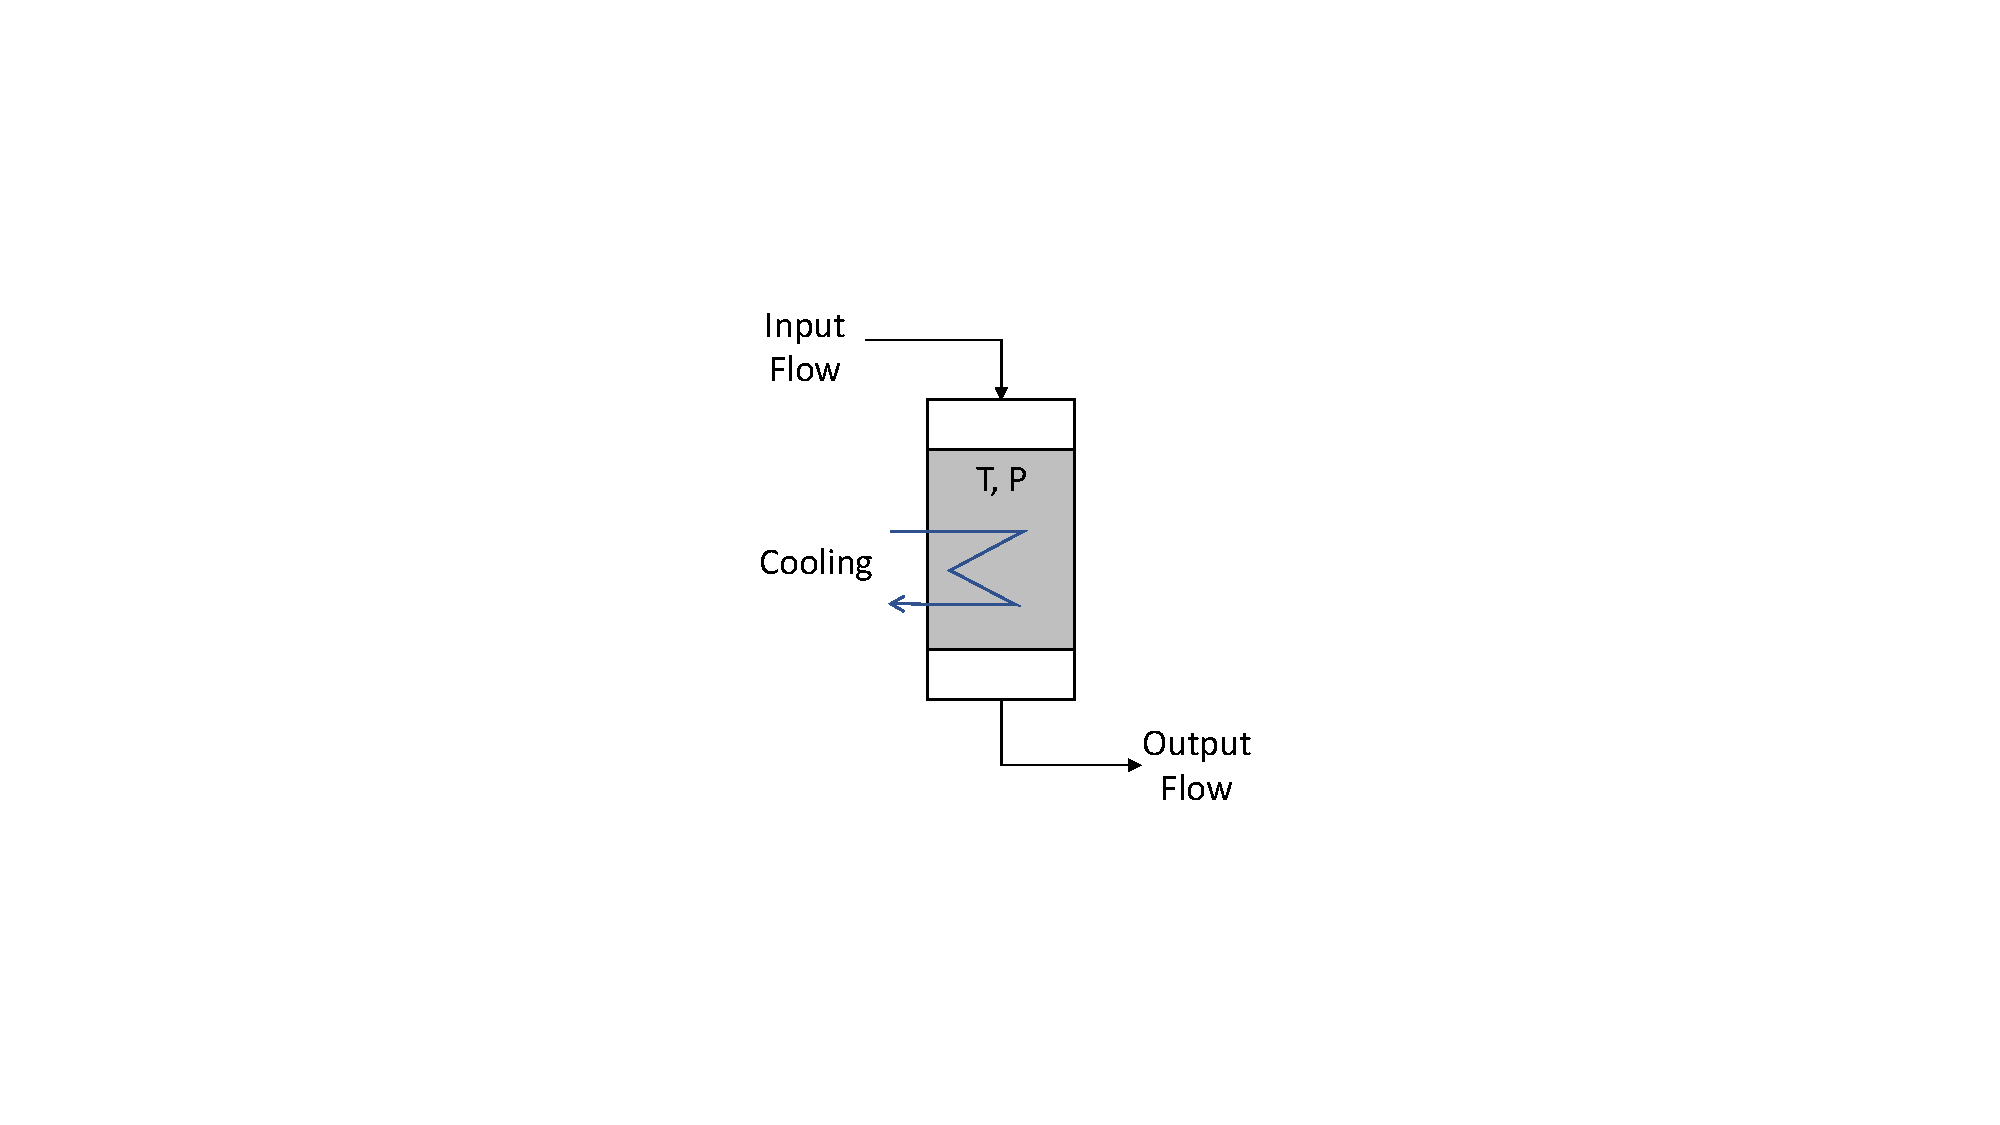
\includegraphics[width=0.4\textwidth]{figstats/gibbs_diagram}
\end{figure}

\begin{block}{}
\begin{itemize}
\item Do you expect a positive or negative correlation between conversion and pressure?
 \item How are output flows for $CO$, $H_2$, and $CH_3OH$ related?
\end{itemize}
\end{block}

\end{frame}
%------------------------------------------------


%------------------------------------------------
%
\begin{frame}{Example: Covariance and Correlation for Reactor}


\begin{figure}[!htb]
    \centering
	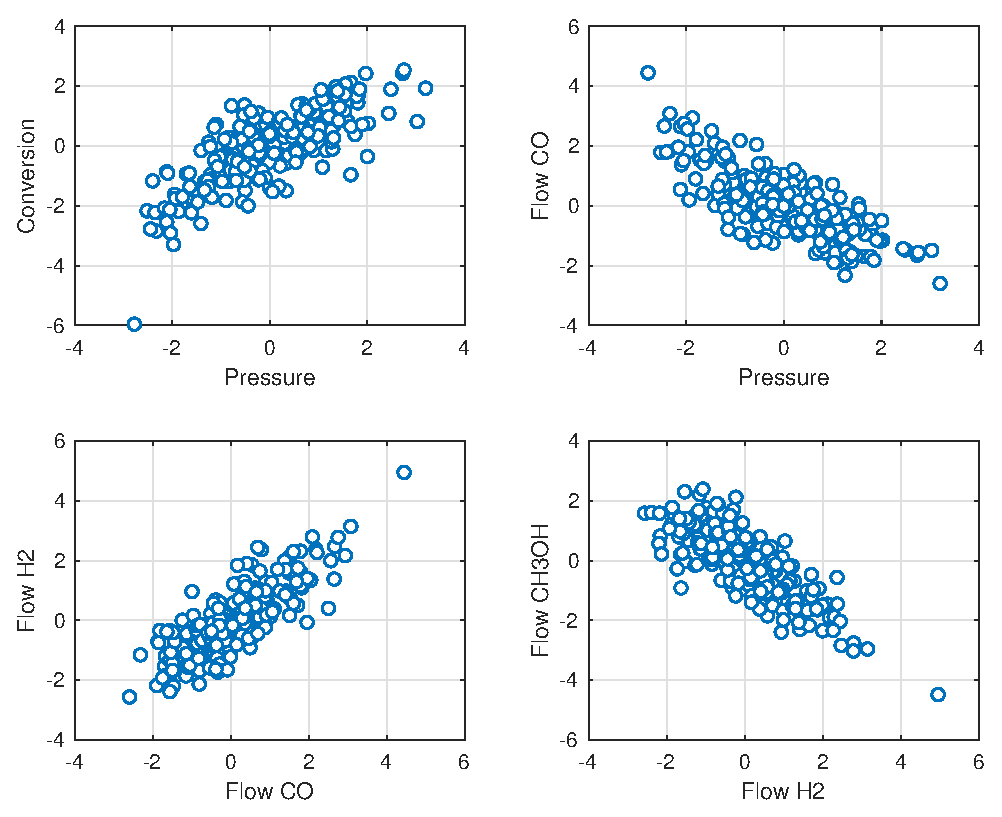
\includegraphics[width=0.7\textwidth]{figstats/Matlab/correlation_gibbs}
\end{figure}



\end{frame}
%------------------------------------------------




%------------------------------------------------
%
\begin{frame}{Covariance and Correlation Matrices}

\begin{itemize}
\item Covariance between variables is often expressed in matrix form as: 
\begin{align*}
\textrm{Cov}[X]=\left[\begin{array}{cc}\sigma_{1,1}&\sigma_{1,2}\\ \sigma_{2,1}&\sigma_{2,2}\end{array}\right]
\end{align*}
this matrix is symmetric because $\sigma_{1,2}=\sigma_{2,1}$ and has positive eigenvalues (it is positive definite).  

\item Covariance matrix (for any dimension $n$) can be computed as:
\begin{align*}
\textrm{Cov}[X]=\mathbb{E}\left[(X-\mathbb{E}[X])(X-\mathbb{E}[X])^T\right]
\end{align*}

\item Correlation between variables is often expressed in matrix form as: 
\begin{align*}
\textrm{Corr}[X]=\left[\begin{array}{cc}1&\rho_{1,2}\\ \rho_{2,1}&1\end{array}\right]
\end{align*}
this matrix is symmetric because $\rho_{1,2}=\rho_{2,1}$ and is positive definite.  

\item Correlation matrix (for any dimension $n$) can be computed as:
\begin{align*}
\textrm{Corr}[X]=D^{-1}\textrm{Cov}(X) D^{-1}
\end{align*}
where $D=\textrm{diag}(\textrm{Cov}[X])$. 
\item Sample covariance and correlation matrices can be computed from data. 
\end{itemize}


\end{frame}
%------------------------------------------------

%------------------------------------------------
%
\begin{frame}{Example: Covariance and Correlation for Reactor}

\begin{itemize}
\item Consider a reactor under which the reaction $CO+2H_2\leftrightarrow CH_3OH$ takes place
\item We have data for pressure, conversion, and output flow of $CO$, $H_2$, and $CH_3OH$
\item Sample covariance and correlation matrices are shown below
\end{itemize}

\begin{align*}
\hat{\textrm{Cov}}[X]=\left[\begin{array}{ccccc}
 		  1.28   &       1.03   &      -0.97    &     -0.90    &      0.96\\
          1.03     &     1.38    &     -1.05    &     -1.00    &      1.04\\
         -0.97      &   -1.05    &      1.20    &      0.98    &     -0.97\\
         -0.90   &      -1.00    &      0.98   &       1.23   &      -0.97\\
          0.96     &     1.04     &    -0.97    &     -0.97   &       1.21
\end{array}\right]
\end{align*}

\begin{align*}
\hat{\textrm{Corr}}[X]=\left[\begin{array}{ccccc}
1.00   &       0.77   &      -0.78   &      -0.71    &      0.77\\
          0.77    &      1.00    &     -0.81    &     -0.77    &      0.81\\
         -0.78   &      -0.81   &       1.00   &       0.81   &      -0.80\\
         -0.71    &     -0.77   &       0.81    &      1.00     &    -0.79\\
          0.77     &     0.81    &     -0.80    &     -0.79    &      1.00
\end{array}\right]
\end{align*}

\begin{block}{}
\begin{itemize}
\item Do you expect a positive or negative correlation between conversion and pressure?
 \item How are output flows for $CO$, $H_2$, and $CH_3OH$ related?
\end{itemize}
\end{block}

\end{frame}
%------------------------------------------------

%------------------------------------------------
%
\begin{frame}{Multivariate Gaussian Variables}

Surprisingly enough, there are actually few established models for multivariate RVs.  The most used model is that of the Gaussian RV, which has a wide range of properties:

\begin{itemize}
\item Consider a multivariate RV vector $X=(X_1,X_2,...,X_n)$.

\item Denote as $X\sim \mathcal{N}(\mu,\Sigma)$, where $\mu\in \mathbb{R}^n$ and $\Sigma\in \mathbb{R}^{n\times n}$ are hyperparameters. 

\item RV $X\sim \mathcal{N}(\mu,\Sigma)$ has joint pdf of the form:
\begin{block}{}
\begin{align*}
f_X(x)=f_X(x_1,x_2,...,x_n)=\frac{1}{(2\pi)^{n/2}|\Sigma|^{1/2}}\exp\left(-\frac{1}{2}(x-\mu)^T\Sigma^{-1}(x-\mu)\right)
\end{align*}
\end{block}
\item $|\Sigma|$ is determinant of  $\Sigma$ (product of its eigenvalues) and $\Sigma$ is positive definite. 

\item Domain of $X$ is $\mathcal{D}=[-\infty,\infty]^n$. 

\item Hyperparameters are given by expected value $\mu=\mathbb{E}[X]$ and covariance $\Sigma=\textrm{Cov}[X]$.

\end{itemize}

\end{frame}
%------------------------------------------------

%------------------------------------------------
%
\begin{frame}{Properties of Multivariate Gaussian RVs}

Consider the case with $n=2$:
\begin{itemize}
\item Can show that marginal pdfs of $X$ are Gaussian:
\begin{block}{}
\begin{align*}
f_1(x_1)&=\int_{x_2\in \mathbb{D}_2}f(x_1,x_2)dx_2=\frac{1}{\sqrt{2\pi\sigma_1^2}}\exp \left({\frac{-(x-\mu_1)^2}{2\sigma_1^2}}\right)\\
f_2(x_2)&=\int_{x_1\in \mathbb{D}_1}f(x_1,x_2)dx_1=\frac{1}{\sqrt{2\pi\sigma_2^2}}\exp \left({\frac{-(x-\mu_2)^2}{2\sigma_2^2}}\right)
\end{align*} 
\end{block}
\item In other words, $X_1\sim\mathcal{N}(\mu_1,\sigma_1^2)$ and $X_2\sim\mathcal{N}(\mu_2,\sigma_2^2)$.
\end{itemize}
\end{frame}
%------------------------------------------------

%------------------------------------------------
%
\begin{frame}{Properties of Multivariate Gaussian RVs}

\begin{itemize}

\item Can show that conditional pdfs of $X$ are Gaussian:
\begin{block}{}
\begin{align*}
f(x_1|x_2)&=\frac{1}{\sqrt{2\pi\sigma_{1|2}^2}}\exp \left({\frac{-(x-\mu_{1|2})^2}{2\sigma_{1|2}^2}}\right)\\
f(x_2|x_1)&=\frac{1}{\sqrt{2\pi\sigma_{2|1}^2}}\exp \left({\frac{-(x-\mu_{2|1})^2}{2\sigma_{2|1}^2}}\right).
\end{align*} 
\end{block}
\item That is, $X_1|X_2\sim \mathcal{N}(\mu_{1|2},\sigma_{1|2})$ and $X_2|X_1\sim \mathcal{N}(\mu_{2|1},\sigma_{2|1})$ with hyperparameters:
\begin{align*}
\mu_{1|2}&=\mu_1+\sigma_{1,2}\sigma_{22}^{-1}(x_2-\mu_2)\\
\sigma_{1|2}&=\sigma_{1,1}-\sigma_{1,2}\sigma_{2,2}^{-1}\sigma_{2,1}\\
\mu_{2|1}&=\mu_2+\sigma_{2,1}\sigma_{1,1}^{-1}(x_1-\mu_1)\\
\sigma_{2|1}&=\sigma_{2,2}-\sigma_{2,1}\sigma_{1,1}^{-1}\sigma_{1,2}
\end{align*}
\item What  if $X_1$ and $X_2$ are independent? What  if they are strongly correlated?
\end{itemize}

\end{frame}
%------------------------------------------------

%------------------------------------------------
%
\begin{frame}{Example: Uncertainty Reduction in Reactor}

\begin{itemize}
\item Consider covariance for pressure $X_1$ and conversion $X_2$ and assume Gaussian.
\item Marginal means are:
\begin{align*}
\mu_1=147\\
\mu_2=0.69
\end{align*}
\item Covariance matrix is:
\begin{align*}
\textrm{Cov}[X]=\left[\begin{array}{cc}  641.31    &      1.84\\
          1.84     &     0.24\end{array}\right]
\end{align*}
\item Marginal variance for conversion is $\sigma_{2,2}=0.24$ (we use this as a measure of its uncertainty).

\item Since pressure and conversion are correlated, we expect that having knowledge of conversion decreases uncertainy in the conversion. To verify this, we compute the variance of conditional density $f(x_2|x_1)$
\begin{align*}
\sigma_{2|1}^2&=(0.24-1.84\cdot (641.31)^{-1}\cdot 1.84)^2\\
&=0.05
\end{align*}
\item Consequently, uncertainty in conversion is reduced by 80\% if we know pressure.  
\item In other words,  since pressure and conversion are correlated, data on pressure carries information on conversion (and the other way around). 

\end{itemize}

\end{frame}
%------------------------------------------------

%------------------------------------------------
%
\begin{frame}{Properties of Multivariate Gaussian RVs}

\begin{itemize}
\item Linear transformation of a multivariate Gaussian is Gaussian: 
\begin{itemize}
\item If $X\sim\mathcal{N}(\mu,\Sigma)$, then $Y=AX+b$ is $Y\sim \mathcal{N}(A\mu+b,A\Sigma A^T)$. 
\end{itemize}
\vspace{0.1in}
\item Linear transformation property is used to establish useful properties:
\begin{itemize}
\item Mixture model:

 If $X_i\sim \mathcal{N}(\mu_i,\sigma_i^2)$, then $Y=\sum_{i=1}^nX_i$ is Gaussian with $Y\sim\mathcal{N}(\sum_{i=1}^n\mu_i,\sum_{i=1}^n\sigma_i^2)$. 
 \vspace{0.1in}
\item Multivariate standard normal: 

If $X\sim\mathcal{N}(0,{I})$ then $Y=\sqrt{\Sigma}X+\mu$ is Gaussian with $Y\sim\mathcal{N}(\mu,\Sigma)$.
\end{itemize}
\item Standarization result used to generate samples of $\mathcal{N}(\mu,\Sigma)$ from samples of $\mathcal{N}(0,I)$.
\end{itemize}

\end{frame}
%------------------------------------------------

%------------------------------------------------
%
\begin{frame}{Example: Gaussian Mixture}
\begin{block}{}
\begin{itemize}
\item Have system with random revenue streams $F_1\sim\mathcal{N}(\mu_1,\sigma_1)$ and $F_2\sim\mathcal{N}(\mu_2,\sigma_2)$
\item Can control amount of revenue using $\kappa_1\in [0,1]$ and $\kappa_2\in [0,1]$
\item What is uncertainty of total revenue $F_3$? How is this affected by $\kappa_1$ and $\kappa_2$? 
\end{itemize}
\end{block}

\begin{figure}[!htb]
    \centering
	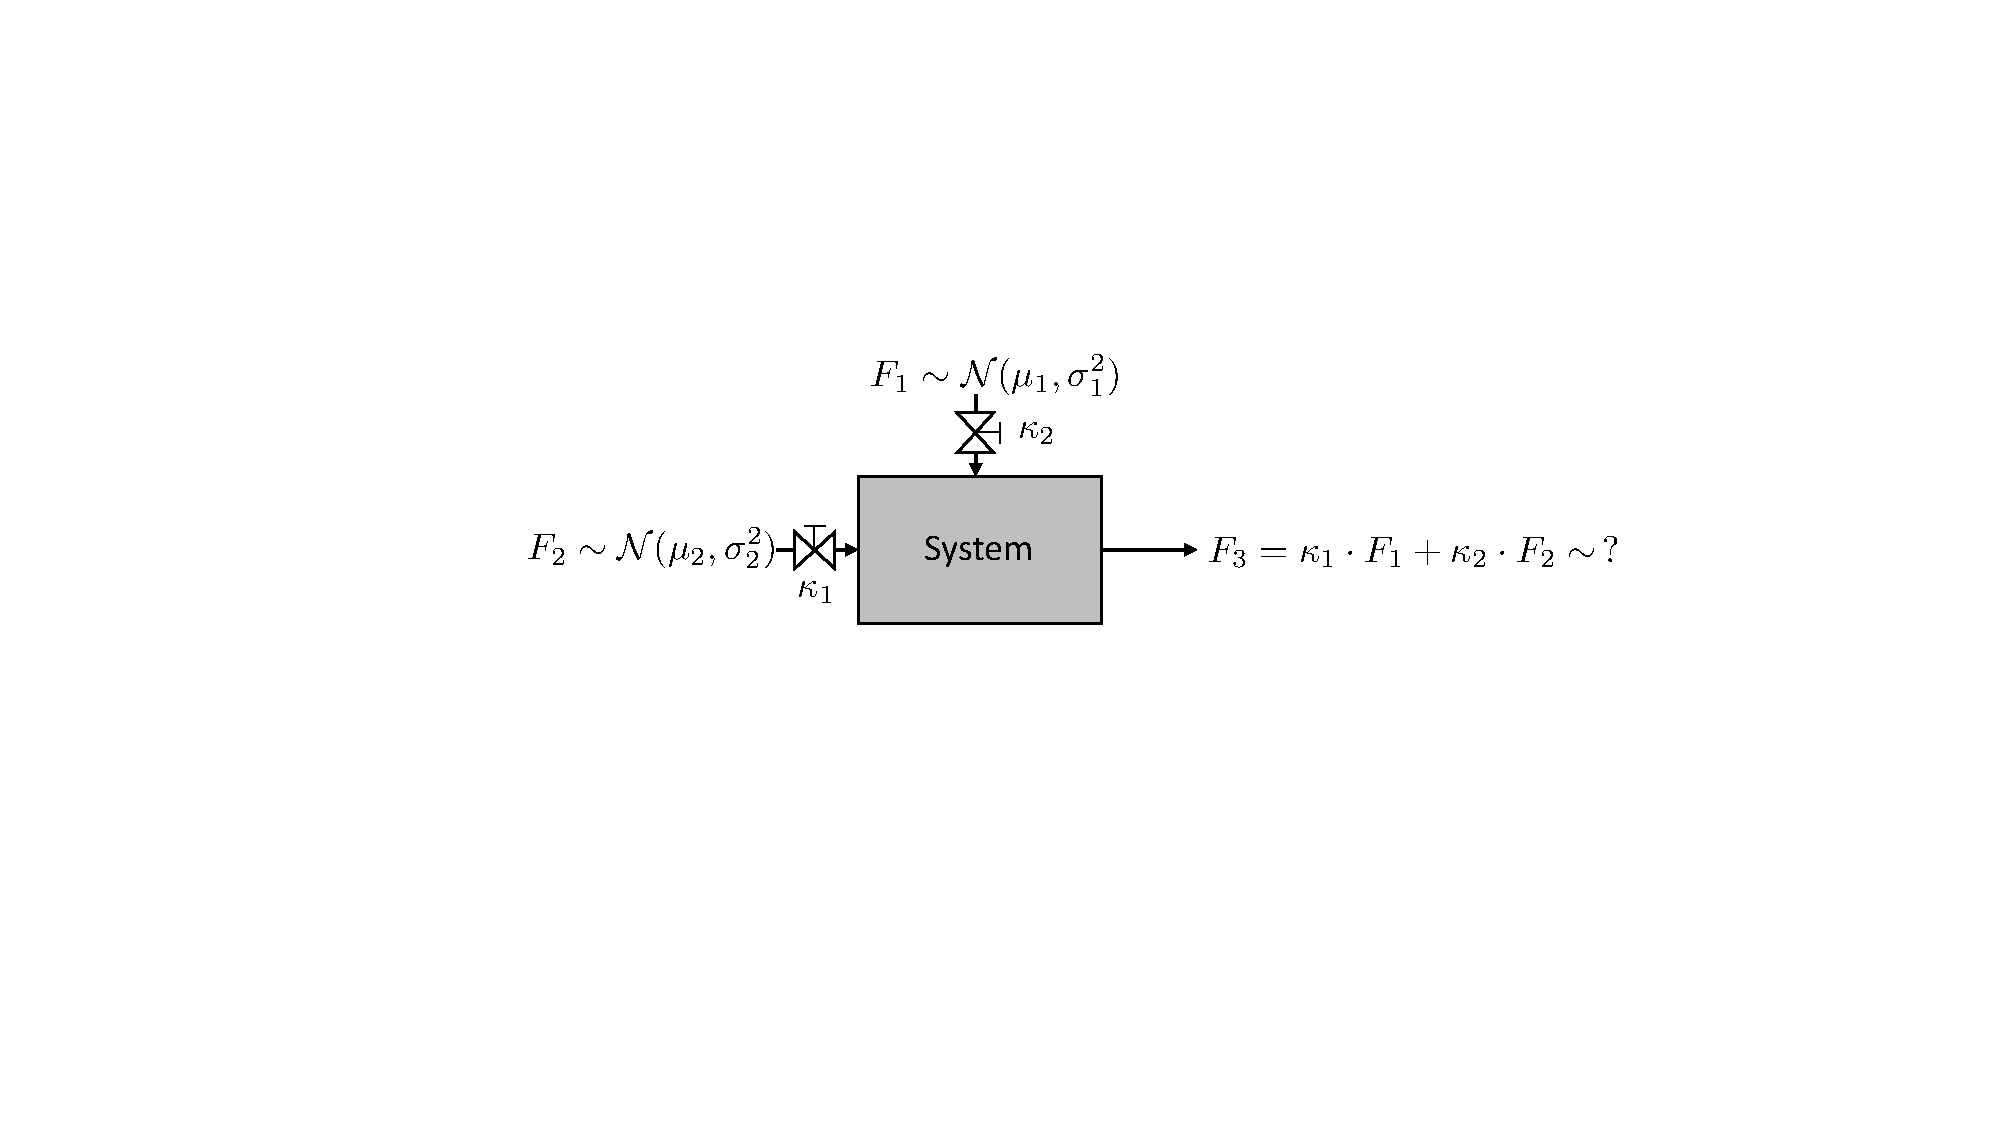
\includegraphics[width=0.7\textwidth]{figstats/gaussian_revenue_diagram}
\end{figure}
\pause 
\begin{itemize}
\item We can write $F_2$ as a linear combination of $F_1$ and $F_2$:
\begin{align*}
F_3=\left[\begin{array}{c} \kappa_1\, \kappa_2
\end{array}\right]\left[\begin{array}{c} F_1\\ F_2
\end{array}\right]=\kappa_1F_1+\kappa_2F_2
\end{align*}
\item We thus have that $F_3\sim\mathcal{N}(\mu_3,\sigma_3)$ with:
\begin{align*}
\mu_3&=\left[\begin{array}{c} \kappa_1\; \kappa_2
\end{array}\right]\left[\begin{array}{c} \mu_1\\ \mu_2
\end{array}\right]=\kappa_1\mu_1+\kappa_2\mu_2\\
\sigma_3^2&=\left[\begin{array}{c} \kappa_1\; \kappa_2
\end{array}\right]\left[\begin{array}{cc} \sigma_1^2&0\\0&\sigma_2^2
\end{array}\right]
\left[\begin{array}{c} \kappa_1\\ \kappa_2
\end{array}\right]=\kappa_1^2\sigma_1^2+\kappa_2^2\sigma_2^2
\end{align*}
\end{itemize}


\end{frame}
%------------------------------------------------

%------------------------------------------------
%
\begin{frame}{Geometry of Multivariate Gaussian Variables}
Understanding geometry of multivariate Gaussian facilitates {\em data visualization}.  

\begin{itemize}
\item For $n=2$ we write joint pdf of $X=(X_1,X_2)$ as:
\begin{align*}
f_X(x_1,x_2)=\frac{1}{2\pi\sigma_1\sigma_2}\exp\left(-U(x_1,x_2)\right)
\end{align*}
where 
\begin{align*}
U(x_1,x_2)=\frac{1}{2(1-\rho^2)}\left[\frac{(x_1-\mu_1)^2}{\sigma_1^2}+\frac{(x_2-\mu_2)^2}{\sigma_2^2}-2\rho\frac{(x_1-\mu_1)(x_2-\mu_2)}{\sigma_1\sigma_2}\right]
\end{align*}

\item If we fix probability $f_X(x_1,x_2)=p$ with $\alpha\in [0,1]$, pdf defines an equation in variables $(x_1,x_2)$.  This is equation of ellipse centered at $\mu_1$ and $\mu_2$.  This ellipse is known as the $p$-level set of pdf.  

\item Correlation coefficient $\rho=\textrm{Corr}(X_1,X_2)$ dictates {\em orientation of ellipse}: if $\rho>0$ this is tilted to right. if $\rho<0$ this is tilted to  left, and if $\rho=0$ ($X_1$ and $X_2$ are independent) ellipse has no tilt. 

\item {\em Length of axes} are dictated by $\sigma_1^2$ and $\sigma_2^2$ (variances of $X_1$ and $X_2$).

\item Maximum value of $f_X(x_1,x_2)$ is achieved at $x_1=\mu_1$ and $x_2=\mu_2$. 

\end{itemize}

\end{frame}
%------------------------------------------------

%------------------------------------------------
%
\begin{frame}{Geometry of Multivariate Gaussian Variables}

\begin{itemize}
\item We are interested in box confidence regions $\mathcal{B}(\alpha)$ satisfying:
\begin{align*}
\mathbb{P}(X\in \mathcal{B}(\alpha))=1-\alpha.
\end{align*}
\item For univariate $X\sim \mathcal{N}(\mu,\sigma^2)$, box region is:
\begin{align*}
\mathcal{B}(\alpha)=\{x\,|\,x\in [\mu\pm \sqrt{\mathbb{Q}(\alpha)} \sigma]\} 
\end{align*}
where $\mathbb{Q}(\alpha)$ is the $\alpha$-quantile of $\chi^2(1)$. 
\item For multivariate $X=(X_1,X_2)$ with $X_1\sim \mathcal{N}(\mu_1,\sigma_1^2)$ and $X_2\sim \mathcal{N}(\mu_2,\sigma_2^2)$ we can build a box of the form:
\begin{align*}
\mathcal{B}(\alpha)=\{(x_1,x_2)\,|\,x_1\in [\mu_1\pm \sqrt{\mathbb{Q}(\alpha)}\sigma_1]\,\&\,x_2\in [\mu_2\pm \sqrt{\mathbb{Q}(\alpha)}\sigma_2]\}.
\end{align*}
\item This box (a.k.a. marginal box) does not capture correlations in $X_1$ and $X_2$. 
\end{itemize}

\end{frame}
%------------------------------------------------


%------------------------------------------------
%
\begin{frame}{Geometry of Multivariate Gaussian Variables}

\begin{itemize}
\item  In multivariate Gaussians, observations concentrate in ellipses ($p$-level sets). We are thus interested in finding {\em ellipsoidal} confidence region $\mathcal{E}(\alpha)$ satisfying:
\begin{align*}
\mathbb{P}(X\in \mathcal{E}(\alpha))=1-\alpha.
\end{align*}
\item For $X\sim \mathcal{N}(\mu,\Sigma)$, the ellipsoidal region is given by:
\begin{align*}
\mathcal{E}(\alpha)=\{x\,|\,(x-\mu)^T\Sigma^{-1}(x-\mu)^T\leq \mathbb{Q}(\alpha)\}.
\end{align*}
where $\mathbb{Q}(\alpha)$ is the $\alpha$-quantile of $\chi^2(n)$.  
\item  Interpretation of region is:
\begin{itemize}
\item If draw a sample from $\mathcal{N}(\mu,\Sigma)$, there is probability $\alpha$ that it will land in $\mathcal{E}(\alpha)$
\item The larger the $\alpha$, the larger the ellipsoid (more likely it is to land in $\mathcal{E}(\alpha)$)
\end{itemize}
\item Tighest box that encloses $\mathcal{E}(\alpha)$ is:
\begin{align*}
\mathcal{B}(\alpha)=\{(x_1,x_2)\,|\,x_1\in [\mu_1\pm \sqrt{\mathbb{Q}(\alpha)}\sigma_1]\,\&\,x_2\in [\mu_2\pm \sqrt{\mathbb{Q}(\alpha)}\sigma_2]\}.
\end{align*}
where $\mathbb{Q}(\alpha)$ is  $\alpha$-quantile of $\chi^2(n)$ (note difference with the marginal box). 
\item Ellipsoidal and enclosing box capture correlations in $X_1$ and $X_2$.
\end{itemize}

\end{frame}
%------------------------------------------------

%------------------------------------------------
%
\begin{frame}{Example: Geometry of Multivariate Gaussian Variables}

Marginal pdfs, joint pdf and confidence ellipse and boxes for Gaussian with correlation. 
\begin{figure}[!htb]
    \centering
	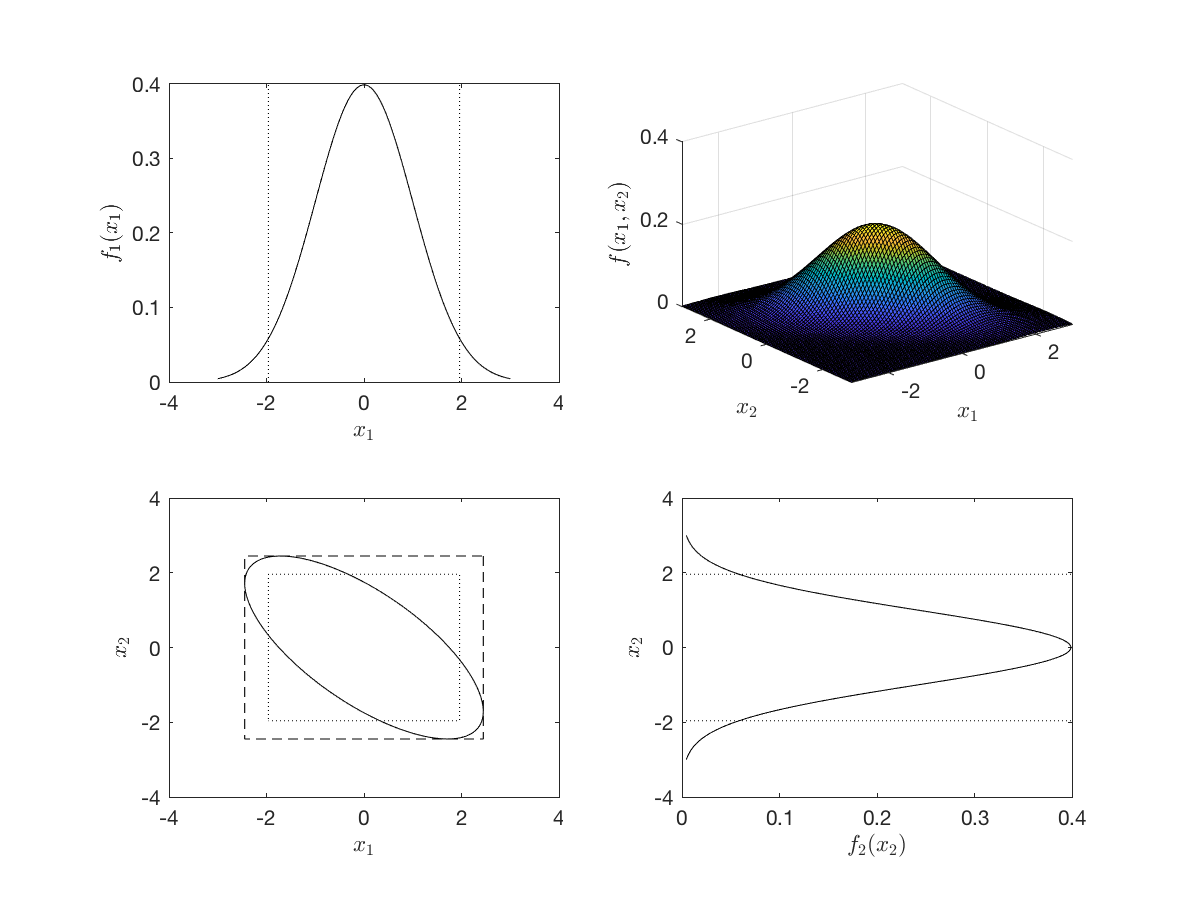
\includegraphics[width=0.7\textwidth]{figstats/Matlab/gaussian_geom_corre}
\end{figure}

\end{frame}
%------------------------------------------------

%------------------------------------------------
%
\begin{frame}{Example: Geometry of Multivariate Gaussian Variables}

Marginal pdfs, joint pdf and confidence ellipse and boxes for Gaussian with no correlation. 
\begin{figure}[!htb]
    \centering
	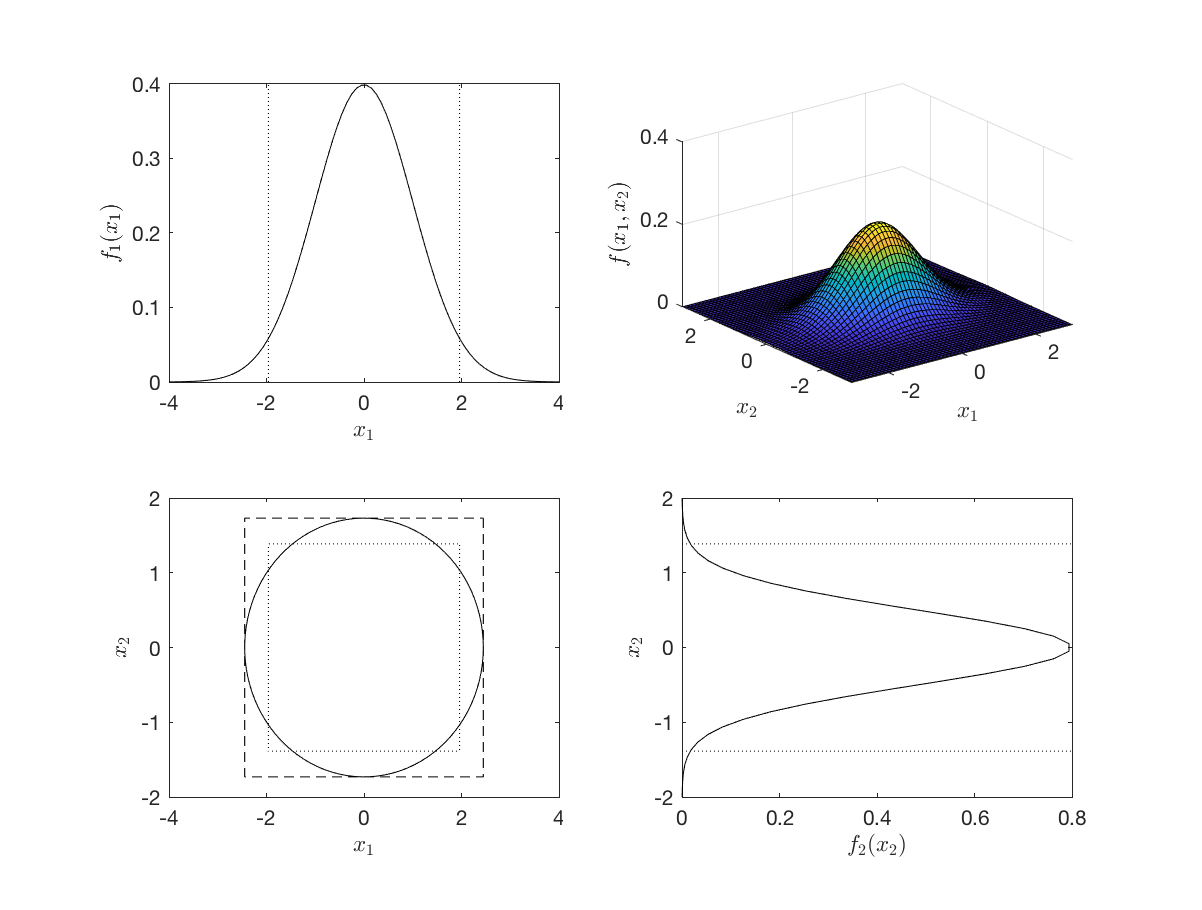
\includegraphics[width=0.7\textwidth]{figstats/Matlab/gaussian_geom_indep}
\end{figure}

\end{frame}
%------------------------------------------------

%------------------------------------------------
%
\begin{frame}{Example: Geometry of Multivariate Gaussian Variables}

\begin{itemize}
\item Here are $S=1000$ observations for Gaussian and $95\%$ confidence ellipsoid
\item Total of 942 samples lie inside of ellipsoid 
\end{itemize}
\begin{figure}[!htb]
    \centering
	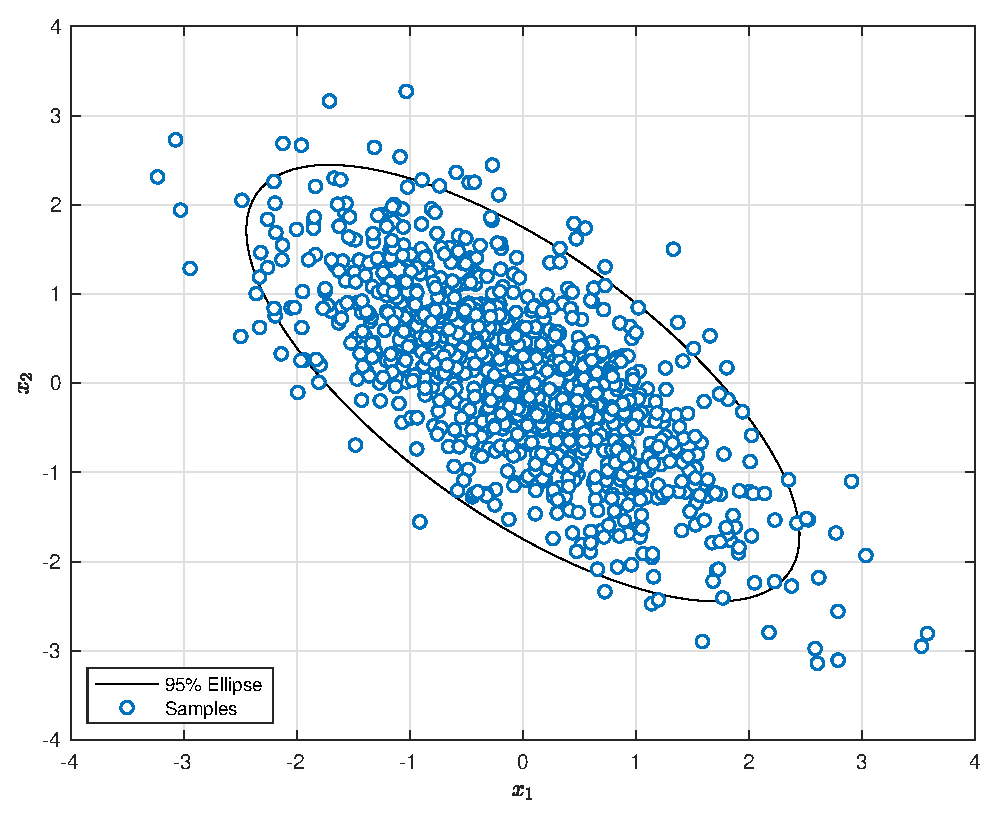
\includegraphics[width=0.7\textwidth]{figstats/Matlab/ellipsoid_points}
\end{figure}

\end{frame}
%------------------------------------------------


%------------------------------------------------
%
\begin{frame}{Data-Driven Modeling}

When $X,Y$ are correlated, variations in $Y$ align with those in $X$ (there is a {\em trend}). 
\begin{block}{}
What if connection is deep (e.g., variations in $Y$ are {\em caused} by variations in $X$)? 
\end{block}

\begin{itemize}

\item Consider univariate RVs $Y$ and $X$ and postulate that any behavior in $Y$ is due to a systematic dependence of $X$:
\begin{align*}
Y=\theta X
\end{align*}
Here, $\theta$ is a parameter that captures a {\em linear} dependence between $X$ and $Y$ . 

\item Use random samples pairs $(y_\omega,x_\omega)$ and, based on postulated model, we assume they are related as:
\begin{align*}
y_\omega=\theta x_\omega + \epsilon_\omega,\; \omega \in \mathcal{S}.
\end{align*}
\item We introduce hidden RV $\epsilon_\omega\in \mathcal{N}(0,\sigma^2)$ with known $\sigma^2$ to capture behavior that cannot be explained by model (the unknown).  

\item  Note $y_\omega$ is an RV because $\epsilon_\omega$ is an RV. Moreover, $y_\omega$ is linear transformation of $\epsilon_\omega$ and thus $y_\omega$ is Gaussian with $\mathbb{E}[y_\omega|x_\omega,\theta]=\theta x_\omega$ and  $\mathbb{V}[y_\omega|x_\omega,\theta]=\sigma^2$. 

\end{itemize}

\end{frame}
%------------------------------------------------

%------------------------------------------------
%
\begin{frame}{Data-Driven Modeling}

\begin{itemize}

\item Recall $f(y_\omega|x_\omega,\theta)$ is probability that $Y=y_\omega$ given that we know $X=x_\omega$ and $\theta$. This is equivalent to assume that $\theta$ and $x_\omega$ are {\em deterministic} (more on this later). 

\item We use a maximum likelihood approach and seek to find $\theta$ that maximizes joint likelihood $\prod_{\omega\in \mathcal{S}}f(y_\omega|x_\omega,\theta)$. This gives:
\begin{block}{}
\begin{align*}
\max_\theta\; \log L(\theta)=\sum_{\omega \in \mathcal{S}} \log f(y_\omega|x_\omega,\theta)
\end{align*}
\end{block}
\item Since $y_\omega\sim \mathcal{N}(\theta x_\omega,\sigma^2)$, we know that:
\begin{block}{}
\begin{align*}
\log f(y_\omega|x_\omega,\theta)=-\log {\sqrt{2\pi\sigma^2}}-{\frac{(y_\omega-\theta x_\omega)^2}{2\sigma^2}}
\end{align*}
\end{block}
\item Terms $\log {\sqrt{2\pi\sigma^2}}$ and $2\sigma^2$ are constants and we thus obtain:
\begin{align*}
\min_\theta \frac{1}{2}\sum_{\omega \in \mathcal{S}} (y_\omega-\theta x_\omega)^2
\end{align*}
This is a least-squares problem and aims to find the estimate ${\theta}$ that minimizes discrepancy between the observed output $y_\omega$ and model prediction ${\theta} x_\theta$. 

\end{itemize}

\end{frame}
%------------------------------------------------

%------------------------------------------------
%
\begin{frame}{Data-Driven Modeling}

We denote best parameter that is {\em learned} from data as $\hat{\theta}$. 
\begin{itemize}
\item Recall $\hat{\theta}$ minimizes $S(\theta)=\frac{1}{2}\sum_{\omega \in \mathcal{S}} (y_\omega-\theta x_\omega)^2$ and thus satisfies:
\begin{align*}
\frac{\partial S(\hat{\theta})}{\partial \theta}=-\sum_{\omega \in \mathcal{S}}x_\omega (y_\omega-\theta x_\omega)=0,\qquad  \frac{\partial^2 S(\hat{\theta})}{\partial \theta^2}>0
\end{align*}
These conditions lead to:
\begin{align*}
\hat{\theta}=\frac{\sum_{\omega \in \mathcal{S}}x_\omega y_\omega}{\sum_{\omega \in \mathcal{S}}x_\omega^2},\qquad \sum_{\omega \in \mathcal{S}}x_\omega^2>0 
\end{align*}
\item Estimate $\hat{\theta}$ captures {\em interactions} in data $x_\omega,y_\omega$. 
\item Estimate $\hat{\theta}$ is {\em unique} and becomes better defined as we add more data. 
\item Recall $y_\omega \sim \mathcal{N}(\hat{\theta} x_\omega,\sigma^2)$, implying that prediction $\hat{\theta} x_\omega$ is the most likely outcome and that the larger $\sigma^2$, the more uncertainty we have in $y_\omega$. 
\item Estimate gives {\em residual noise estimates} $\hat{\epsilon}_\omega =y_\omega-\hat{\theta}x_\omega$. If these estimates follow our assumption $\mathcal{N}(0,\sigma^2)$ then the available data and postulated model is satisfactory. If not, more data or another model is needed (e.g., nonlinear). 

\item From $y_\omega=\hat{\theta}x_\omega+\epsilon_\omega$ we note that model $\hat{\theta}x_\omega$ represents what we know about $y_\omega$ while $\epsilon_\omega$ represents the unknown. Estimation problem thus seeks to extract maximum knowledge from data (minimize the unknown). 
\end{itemize}
\end{frame}
%------------------------------------------------

%------------------------------------------------
%
\begin{frame}{Data-Driven Modeling}

\begin{figure}[!htb]
    \centering
	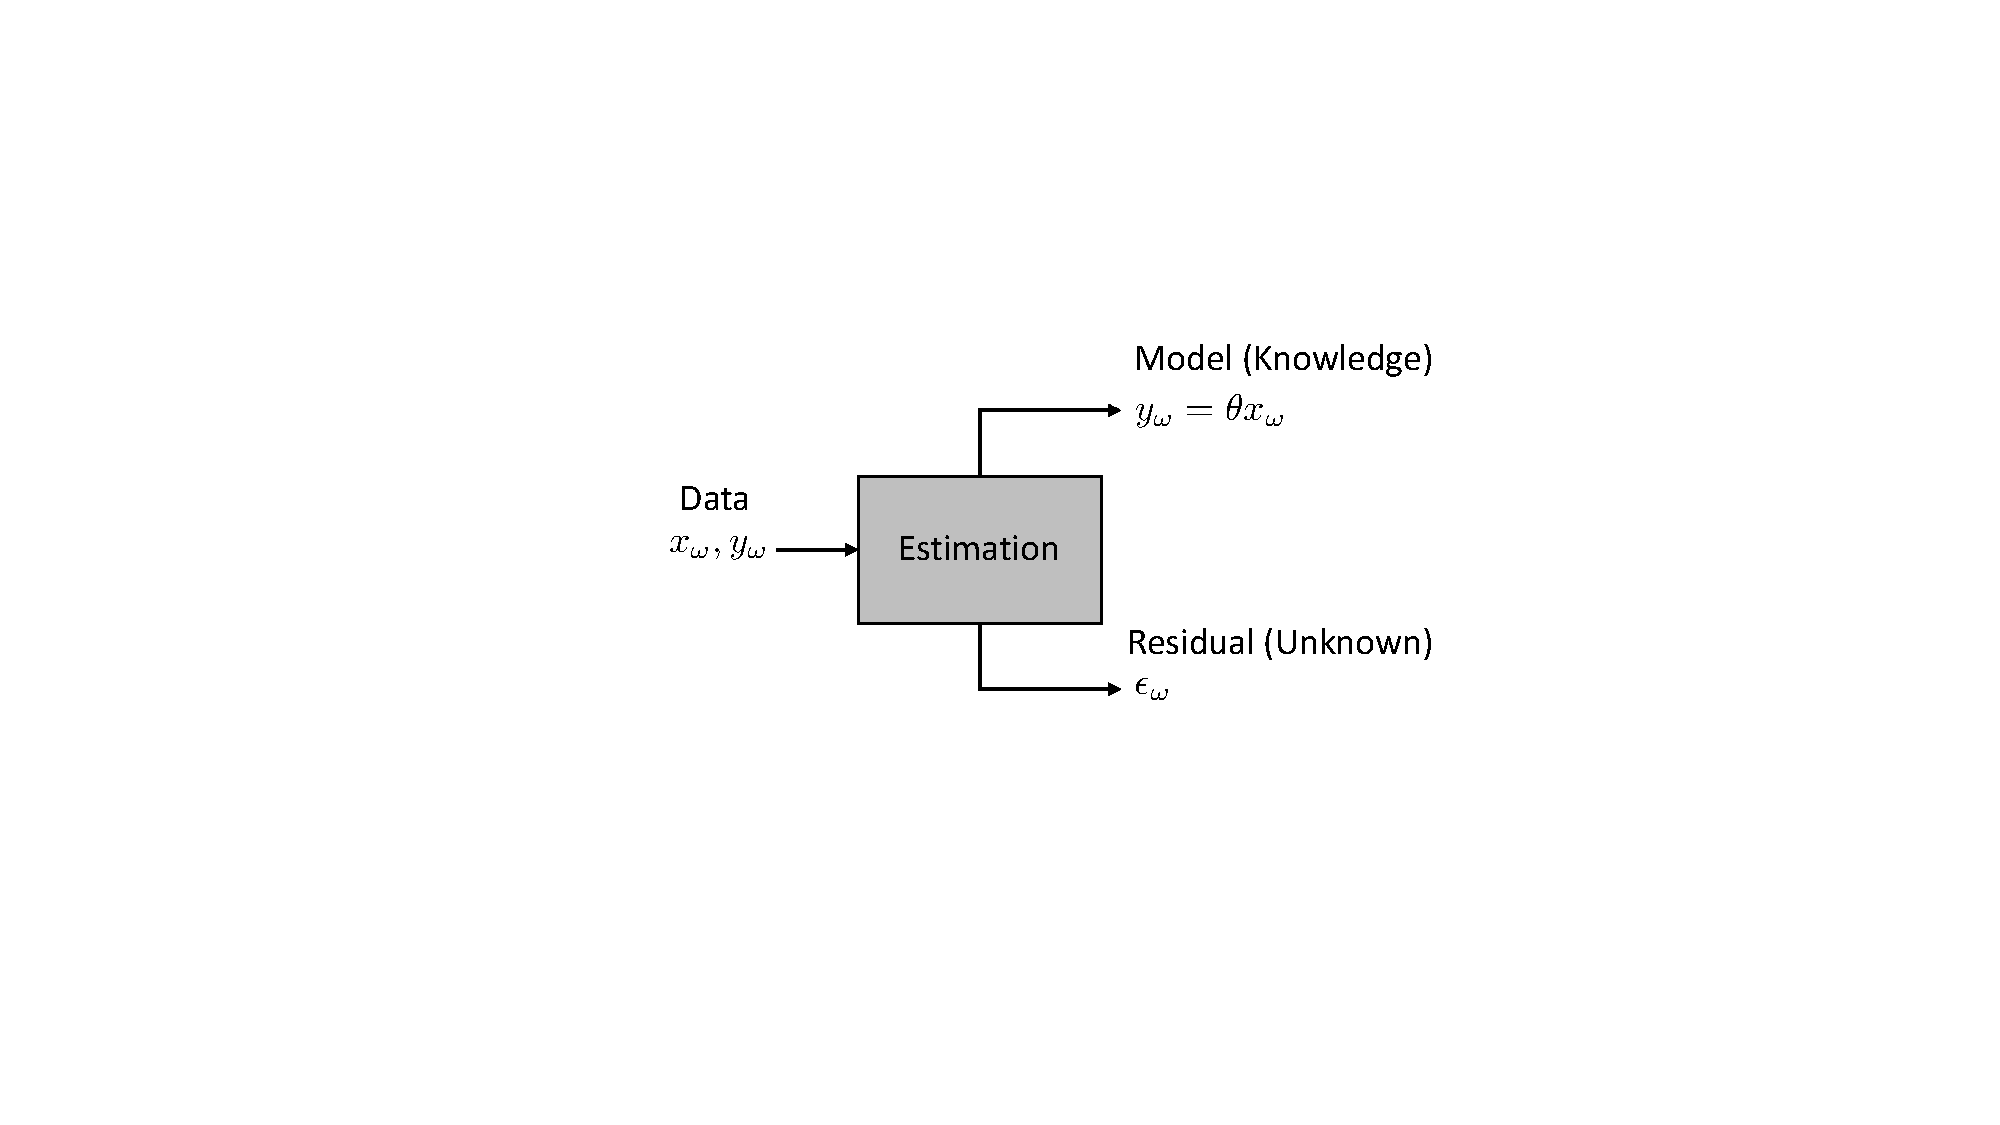
\includegraphics[width=0.7\textwidth]{figstats/knowledge_extraction_diagram}
\end{figure}

\end{frame}
%------------------------------------------------

%------------------------------------------------
%
\begin{frame}{Example: Data-Driven Modeling}

\begin{block}{}
\begin{itemize}
\item Consider input out pair data $(Y,X)$ with true relationship $Y=\theta X$ and $\theta=2$
\item Observations $(y_\omega,x_\omega)$ are corrupted by noise $\epsilon_\omega  \sim \mathcal{N}(0,0.25)$
\item If we use $S=100$ observations, best estimate is $\hat{\theta}=1.96$ 
\end{itemize}
\end{block}

\begin{figure}[!htb]
    \centering
	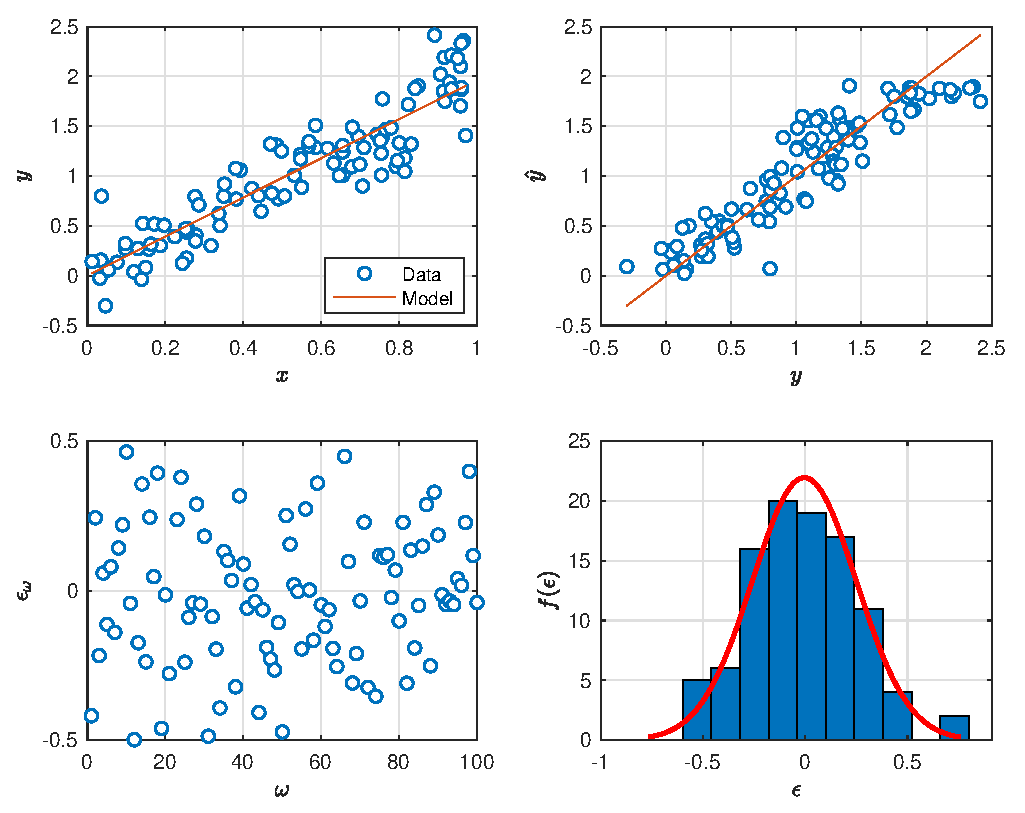
\includegraphics[width=0.6\textwidth]{figstats/Matlab/results_lin_est}
\end{figure}

\end{frame}
%------------------------------------------------

%------------------------------------------------
%
\begin{frame}{Example: Data-Driven Modeling}

\begin{block}{}
\begin{itemize}
\item Below we show function $S(\theta)$ for different amounts of data $S=10,100,1000$
\item Note how surface becomes better defined as we add data
\end{itemize}
\end{block}

\begin{figure}[!htb]
    \centering
	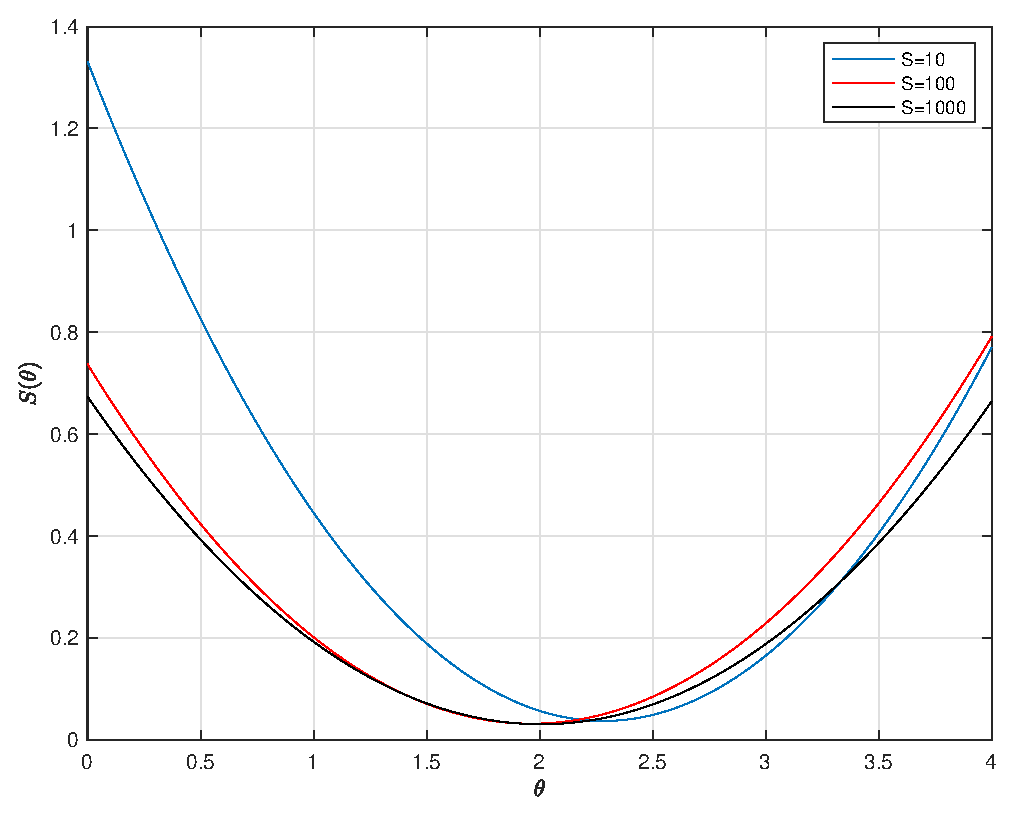
\includegraphics[width=0.7\textwidth]{figstats/Matlab/sharpness_lin_est}
\end{figure}

\end{frame}
%------------------------------------------------


%------------------------------------------------
%
\begin{frame}{Example: Data-Driven Modeling}

\begin{block}{}
\begin{itemize}
\item Assume now true relationship $Y=\theta X^2$ and $\theta=2$
\item Below we show model predictions if we postulate wrong model $Y=\theta X$
\end{itemize}
\end{block}

\begin{figure}[!htb]
    \centering
	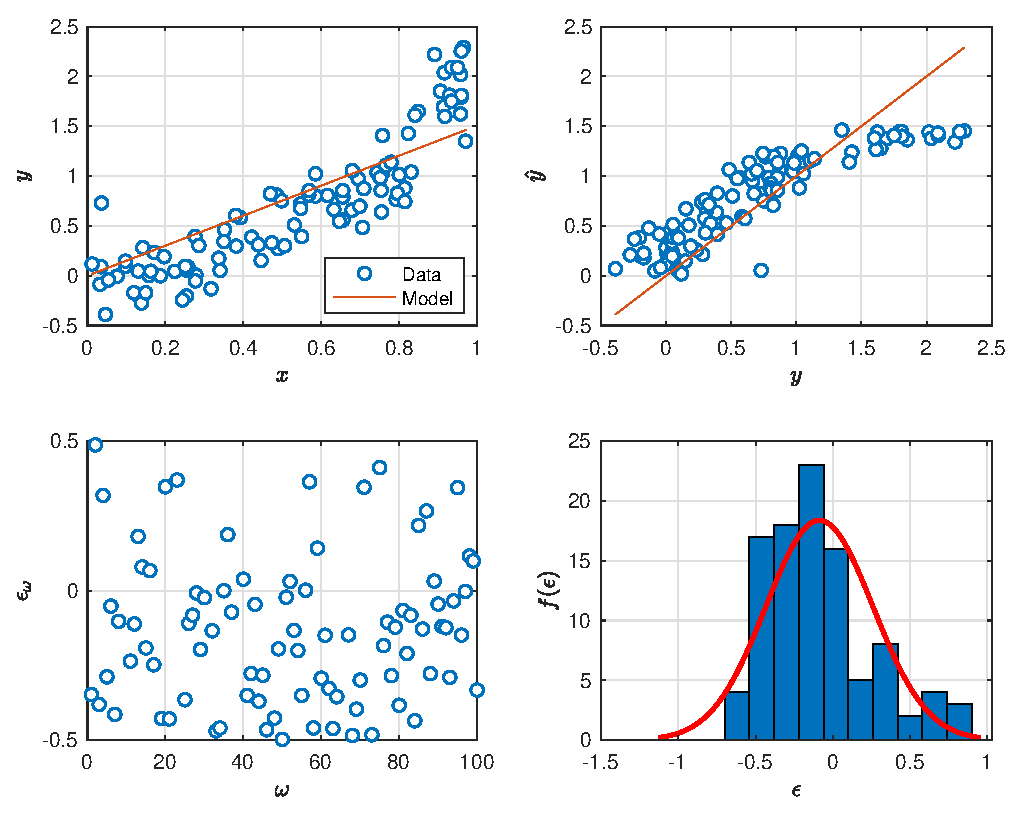
\includegraphics[width=0.6\textwidth]{figstats/Matlab/results_lin_est_wrong}
\end{figure}

\begin{itemize}
\item Residual statistics play key role in determining appropriateness of postulated model.
\end{itemize}

\end{frame}
%------------------------------------------------

%------------------------------------------------
%
\begin{frame}{Data-Driven Modeling}

Now generalize linear model to account for influence of multiple inputs. We postulate:
\begin{align*}
Y&=\theta_0+\sum_{i=1}^n\theta_iX_i
\end{align*}
Use samples (data) pairs $(y_\omega,x_\omega)$ and, based on postulated model, we have that:
\begin{align*}
y_\omega=\theta_0+\sum_{i=1}^n\theta_i x_{i,\omega} + \epsilon_\omega,\; \omega \in \mathcal{S}.
\end{align*}
These set of equations can be expressed compactly using matrix notation:
\begin{align*}
\mathbf{y}=\mathbf{X}\theta + \epsilon
\end{align*}
where:
\begin{align*}
\mathbf{y}=\left[\begin{array}{c}y_1\\y_2\\\vdots \\ y_S\end{array}\right]\quad 
\mathbf{X}=\left[\begin{array}{ccccc}1&x_{1,1}&x_{1,2}&\hdots&x_{1,n}\\
1&x_{2,1}&x_{2,2}&\hdots&x_{2,n}\\
\vdots&&&\vdots\\
1&x_{S,1}&x_{S,2}&\hdots&x_{S,n}\\
\end{array}\right]\quad \mathbf{\theta}=\left[\begin{array}{c}\theta_0\\\theta_1\\\vdots \\ \theta_n\end{array}\right]\quad 
\quad \mathbf{\epsilon}=\left[\begin{array}{c}\epsilon_1\\\epsilon_2\\\vdots \\ \epsilon_S\end{array}\right]\quad 
\end{align*}
We assume unknown noise is $\epsilon\sim \mathcal{N}(0,\Sigma)$ with $\Sigma_{\omega,\omega}=\sigma^2$ for $\omega\in\mathcal{S}$. 

\end{frame}
%------------------------------------------------



%------------------------------------------------
%
\begin{frame}{Data-Driven Modeling}

Best estimate $\hat{\theta}$ is found as the solution of max likelihood problem:
\begin{align*}
\min_{\theta}&\quad \frac{1}{2}(\mathbf{y}-\mathbf{X}\theta)^T (\mathbf{y}-\mathbf{X}\theta)
\end{align*}
Problem can also be written as:
\begin{align*}
\min_{\theta}&\quad \frac{1}{2}\|\mathbf{y}-\mathbf{X}\theta\|^2
\end{align*}
Solution of this problem must satisfy:
\begin{align*}
\frac{\partial S(\theta)}{\partial \theta} &= -\mathbf{X}^T(\mathbf{y}-\mathbf{X}\theta)=0\\
\left|\frac{\partial^2 S(\theta)}{\partial \theta^2}\right| &= \left|\mathbf{X}^T\mathbf{X}\right|>0
\end{align*}
First condition yields:
\begin{align*}
\hat{\theta}=(\mathbf{X}^T\mathbf{X})^{-1}\mathbf{X}^T\mathbf{y}.
\end{align*}
Second condition indicates that $\hat{\theta}$ is unique if matrix $\mathbf{X}^T\mathbf{X}$ is positive definite. 

\end{frame}
%------------------------------------------------

%------------------------------------------------
%
\begin{frame}{Data-Driven Modeling}

Now note that $\mathbf{y}=\mathbf{X}\theta+\epsilon$ is an RV ($\theta$ is true parameter). Consequently: 
\begin{align*}
\hat{\theta}&=(\mathbf{X}^T\mathbf{X})^{-1}\mathbf{X}^T(\mathbf{X}\theta+\epsilon)\\
&=(\mathbf{X}^T\mathbf{X})^{-1}(\mathbf{X}^T\mathbf{X})\theta+(\mathbf{X}^T\mathbf{X})^{-1}\mathbf{X}^T\epsilon\\
&=\theta+(\mathbf{X}^T\mathbf{X})^{-1}\mathbf{X}\epsilon
\end{align*}
Estimate $\hat{\theta}$ is thus an RV (a linear transformation of noise $\epsilon\sim\mathcal{N}(0,\Sigma)$)  and thus:
\begin{align*}
\hat{\theta}\sim\mathcal{N}(\theta,(\mathbf{X}^T\mathbf{X})^{-1}\sigma^2)
\end{align*}
Some observations:
\begin{itemize}
\item Expected value of estimate is $\mathbb{E}[\hat{\theta}]=\theta$ (estimate is unbiased).
\item Covariance of estimate is $\textrm{Cov}[\theta]=(\mathbf{X}^T\mathbf{X})^{-1}\sigma^2$. As variance $\sigma^2$ increase so does variance of $\theta$ (covariance is sensitivity of estimates to noise).
\end{itemize}
\end{frame}
%------------------------------------------------

%------------------------------------------------
%
\begin{frame}{Data-Driven Modeling}

\begin{block}{}
How much of the variability in the data $\mathbf{y}$ can be explained by our gained knowledge (model $\hat{\mathbf{y}}=\mathbf{X}^T\hat{\theta}$) and how much of it cannot be explained (unknown $\epsilon$)?
\end{block}
This can be addressed using {\em analysis of variance} (ANOVA).  Total variability of data is:
\begin{align*}
S_{y}=\sum_{\omega\in \mathcal{S}}(y_\omega -\bar{{y}})^2\quad \textrm{with}
\quad \bar{{y}}=\frac{1}{S}\sum_{\omega \in \mathcal{S}}y_\omega 
\end{align*}
Total variability can be decomposed into contributions as:
\begin{align*}
S_{y}=\underbrace{\sum_{\omega\in \mathcal{S}}(\hat{y}_\omega -\bar{y})^2}_{S_m}+\underbrace{\sum_{\omega\in \mathcal{S}}(y_\omega -\hat{y}_\omega)^2}_{S_e}
\end{align*}
Here, $S_m$ is known as model sum of squares and $S_e$ is known as sum of squared errors.  Based on these quantities we define index: 
\begin{align*}
R^2&=\frac{S_m}{S_y}=1-\frac{S_e}{S_y}
\end{align*}
This represents faction of variability captured by model. The fraction that is left unexplained is $1-R^2={S_e}/{S_y}$.  Consequently, $R^2\to 1$ indicates model fully explains data variability. 
\end{frame}
%------------------------------------------------

%------------------------------------------------
%
\begin{frame}{Data-Driven Modeling}

\begin{block}{}
How confident are we in estimate $\hat{\theta}$ and in model predictions $\hat{\mathbf{y}}=\mathbf{X}\hat{\theta}$?
\end{block}
\begin{itemize}
\item We have established that $\hat{\theta}\sim\mathcal{N}(\theta,(\mathbf{X}^T\mathbf{X})^{-1}\sigma^2)$.  We thus have that true $\theta$ lies in region $\mathcal{E}(\alpha)$ defined by:
\begin{align*}
(\hat{\theta}-\theta)^T\left(\frac{\mathbf{X}^T\mathbf{X}}{\sigma^2}\right)(\hat{\theta}-\theta)\leq \mathbb{Q}(\alpha)
\end{align*}
where $\mathbb{Q}(\alpha)$ is $\alpha$-quantile of $\chi^2(n+1)$.  

\item In most scientific literature, confidence in estimates is reported using marginals:
\begin{align*}
\hat{\theta}_i\sim \mathcal{N}(\theta_i,\sigma^2(\mathbf{X}\mathbf{X})^{-1}_{ii}),\; i=0,...,n
\end{align*}
as:
\begin{align*}
\theta_i=\hat{\theta}_i\pm m_i\;\qquad m_i=\sqrt{\mathbb{Q}(\alpha)\sigma^2(\mathbf{X}\mathbf{X})^{-1}_{ii}}\;
\end{align*}
where  $\mathbb{Q}(\alpha)$ is $\alpha$-quantile of $\chi^2(1)$. This disregards correlations in parameters. 
\item We can construct confidence intervals for model predictions by noticing that $\mathbf{\hat{y}}=\mathbf{X}\hat{\theta}$ and $\hat{\theta}\sim\mathcal{N}(\theta,(\mathbf{X}^T\mathbf{X})^{-1}\sigma^2)$ and thus:
\begin{align*}
\hat{\mathbf{y}}\sim \mathcal{N}(\mathbf{y},\mathbf{X}(\mathbf{X}^T\mathbf{X})^{-1}\mathbf{X}^T\sigma^2)
\end{align*} 
\end{itemize}
\end{frame}
%------------------------------------------------

%------------------------------------------------
%
\begin{frame}{Example: Catalytic Reactor}

\begin{block}{}
\begin{itemize}
\item Given experimental data for pressure $X_1$, temperature $X_2$, and conversion $Y$ 
\item Total of $S=32$ observations
\end{itemize}
\end{block}


\begin{figure}[!htb]
    \centering
	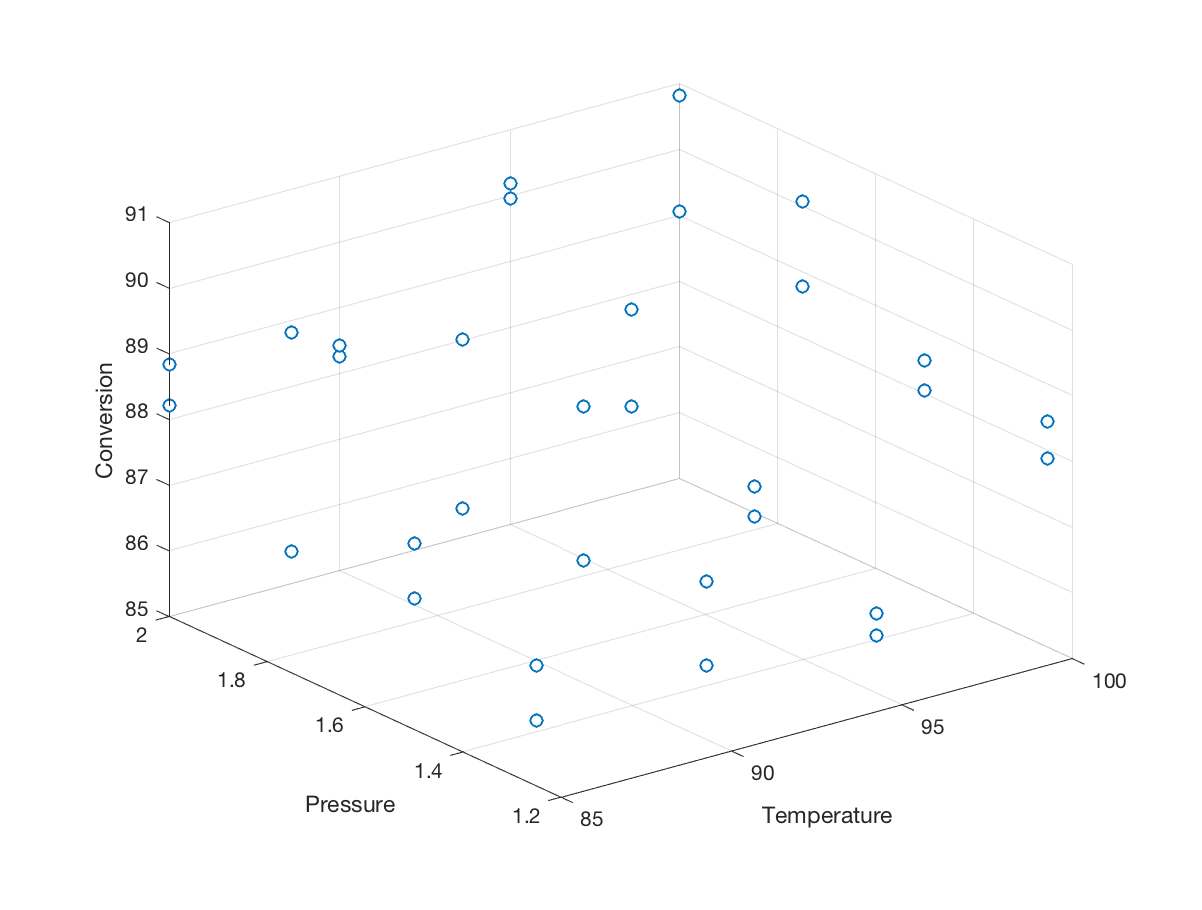
\includegraphics[width=0.7\textwidth]{figstats/Matlab/data_reactor}
\end{figure}

\end{frame}
%------------------------------------------------

%------------------------------------------------
%
\begin{frame}{Example: Catalytic Reactor}

\begin{block}{}
\begin{itemize}
\item We postulate model $Y=\theta_0+\theta_1X_1 + \theta_2 X_2$ with noise model $\epsilon \sim \mathcal{N}(0,\sigma)$
\item Model fit and residual pdf is shown below 
\end{itemize}
\end{block}


\begin{figure}[!htb]
    \centering
	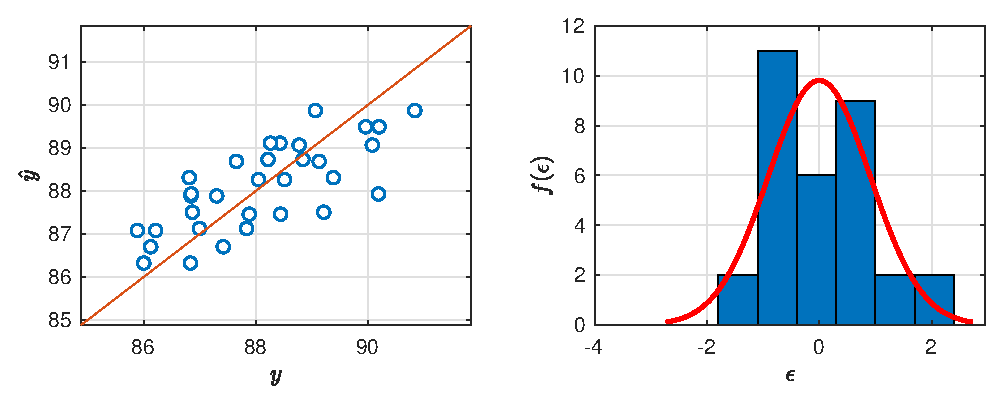
\includegraphics[width=0.6\textwidth]{figstats/Matlab/model_reactor}
\end{figure}

\begin{itemize}
\item $R^2=0.55$ (55\% of total variability is explained by model)
\item Parameters $95\%$ confidence intervals (marginals) are:
\begin{align*}
 \theta_0&\in [69.8858, \,81.8434]\\ 
 \theta_1&\in  [0.0149,\,    0.1366]\\
  \theta_2&\in [1.9946,\,   4.4299]
\end{align*}
\end{itemize}
\begin{block}{}
\begin{center}
Model seems satisfactory, low $R^2$ suggests that measurements are inaccurate. 
\end{center}
\end{block}

\end{frame}
%------------------------------------------------



%------------------------------------------------
%
\begin{frame}{Data-Driven Modeling}

\begin{block}{}
Is the available data sufficient (or too much) to construct model?
\end{block}
Some observations on having sufficient data:
\begin{itemize}
\item Matrix $\mathbf{X}^T\mathbf{X}$ plays a fundamental role as it contains all input data and determines  sharpness of minimum and variance of estimate $\hat{\theta}$. 
\begin{itemize}
\item If one or more eigenvalues of $\mathbf{X}^T\mathbf{X}$ are large, $\hat{\theta}$ is well-defined by the data and its variance is small.  This manifests as a sharp minimum $S(\hat{\theta})$. 
\item If one or more eigenvalues of $\mathbf{X}^T\mathbf{X}$ are close to zero, $\hat{\theta}$ is ill-defined by the data and variance is large. This manifests as a flat minimum $S(\hat{\theta})$. 
\item If one eigenvalue of $\mathbf{X}^T\mathbf{X}$ is zero, $\hat{\theta}$ cannot be resolve uniquely from data.  
\end{itemize}
\item Volume of data is not sufficient, we also require {\em quality of data}. 
\begin{itemize}
\item Observations do not provide information if redundant ($\mathbf{X}^T\mathbf{X}$ has dependent rows). 
\item If selected inputs $X$ do not explain output $\mathbf{y}$ estimates $\hat{\theta}$ might exhibit high variability (regardless of number of observations). 
\item Using knowledge of application to select input variables is important.  
\end{itemize}
\item Selection of input variables and observations is a topic of {\em design of experiments}. 
\item Inputs $X$ are a.k.a. {\em regressor variables}, {\em explanatory variables}, {\em features}, or {\em descriptors}. 
\end{itemize}

\end{frame}
%------------------------------------------------

%------------------------------------------------
%
\begin{frame}{Data-Driven Modeling}

\begin{block}{}
Is the available data sufficient (or too much) to construct model?
\end{block}
Some observations on using excessive data:
\begin{itemize}
\item A common issue is that we use too many inputs $X$ to explain output $Y$. This can result in a large number of parameters and {\em overfitting}. 
\item Check that $\hat{\theta}$ obtained with observations $(y_\omega,x_\omega),\; \omega \in \mathcal{S}$ predicts well in an independent set of observations $(y_\omega,x_\omega),\; \omega \in \mathcal{T}$. This procedure is called {\em cross-validation} or out-of-sample testing. 
\item Cross validation will ensure that model is {\em generalizable}. 
\item In linear models, and adjusted $R^2$ index is used to account for number of parameters:
\begin{align*}
R^2_{adj}=1-\frac{S_e}{S_y}\frac{(S-1)}{(S-n)}
\end{align*}
As number of parameters $n$ increases, we have that $R^2_{adj}$ decreases. 
\item Note that the size of confidence ellipsoid $\mathcal{E}(\theta)$ depends on $n$.
\item A strategy to deal with many parameters is {\em regularization} (will be covered later). Regularization seeks to embed {\em prior} knowledge in estimation problem. 
\end{itemize}

\end{frame}
%------------------------------------------------

%------------------------------------------------
%
\begin{frame}{Example: Catalytic Reactor}

\begin{itemize}
\item $R^2=0.55$, $R^2_{adj}=0.52$ (model does not seem overparameterized)
\item Below we show confidence ellipses for $S=32$ (all data) and $S=16$ (reduced data). This tells us that there is a bit of redundancy in data. 
\end{itemize}

\begin{figure}[!htb]
    \centering
	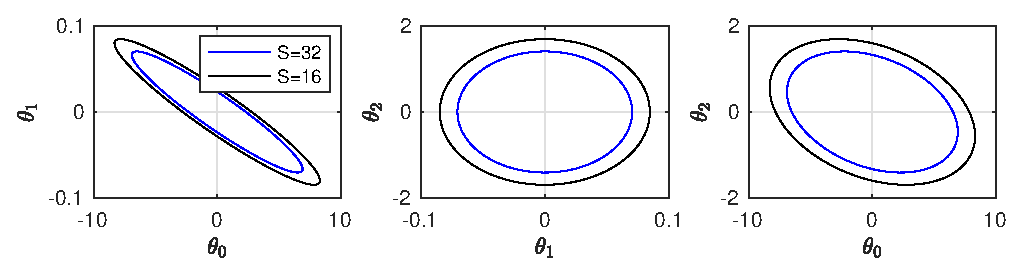
\includegraphics[width=0.9\textwidth]{figstats/Matlab/ellipsoids_reactor}
\end{figure}

\end{frame}
%------------------------------------------------

%------------------------------------------------
%
\begin{frame}{Data-Driven Modeling (Nonlinear)}

Now generalize the linear model to a general model of the form:
\begin{align*}
y_\omega=g(\theta, x_{\omega}) + \epsilon_\omega,\; \omega \in \mathcal{S}.
\end{align*}
where $g:\mathbb{R}^{n}\times \mathbb{R}^S\to \mathbb{R}$ is a model function of the parameters and inputs. 

\begin{itemize}
\item The model function can be nonlinear and capture mechanistic relationships between the inputs, parameters, and outputs. 

\item In linear case we have $g(\theta,x_\omega)=\theta_0+\sum_{i=1}^n\theta_i x_{i,\omega} + \epsilon_\omega$. 

\item Use an MLE framework to estimate $\theta$:
\begin{align*}
\min_{\theta} \; S(\theta)=\frac{1}{2}\sum_{\omega \in \mathcal{S}}(y_\omega - m_\omega(\theta))
\end{align*}
where $m_\omega(\theta)=g(\theta, x_{\omega})$.  Problem can be expressed in vector form:
\begin{align*}
\min_{\theta} \; \frac{1}{2}\|\mathbf{y} - \mathbf{m}(\theta)\|^2
\end{align*}
\item Solution $\hat{\theta}$ satisfies following set of $n$ nonlinear equations (a.k.a. score functions):
\begin{align*}
\nabla_\theta S(\theta)=0\qquad \Longleftrightarrow\qquad  \nabla_\theta m(\theta)^T(\mathbf{y}-\mathbf{m}(\theta))=0
\end{align*}
\end{itemize}
\end{frame}
%------------------------------------------------


%------------------------------------------------
%
\begin{frame}{Nonlinear Estimation}

\begin{itemize}
\item Solution $\hat{\theta}$ also satisfies $|\mathbf{H}({\theta})|>0$ where:
\begin{footnotesize}
\begin{align*}
\mathbf{H}(\theta)=\frac{\partial^2 S(\theta)}{\partial \theta^2}=
\left[\begin{array}{ccccccccc}
\frac{\partial^2 S(\theta)}{\partial \theta_1\partial \theta_1}&\frac{\partial^2 S(\theta)}{\partial \theta_1\partial \theta_2}&\cdots& \frac{\partial^2 S(\theta)}{\partial \theta_1\partial \theta_n}\\
\frac{\partial^2 S(\theta)}{\partial \theta_1\partial \theta_2}&\frac{\partial^2 S(\theta)}{\partial \theta_2\partial \theta_2}&\cdots&\frac{\partial^2 S(\theta)}{\partial \theta_n\partial \theta_2}\\
\vdots & \vdots &\vdots &\vdots\\
\frac{\partial^2 S(\theta)}{\partial \theta_1\partial \theta_n}&\frac{\partial^2 S(\theta)}{\partial \theta_2\partial \theta_n}&\cdots& \frac{\partial^2 S(\theta)}{\partial \theta_n\partial \theta_n}
\end{array}\right]
\end{align*}
\end{footnotesize}
This matrix is known as the {\em Hessian} matrix. 
\item For linear models the Hessian is:
\begin{align*}
\mathbf{H}(\theta)=X^TX
\end{align*}
because  $\nabla_\theta m(\theta)=X$.  
\item As in linear case, eigenvalues of Hessian matrix encode information about data quality and quantity. 
\item What is different about nonlinear estimation?
\begin{itemize}
\item  Difficult to obtain pdf of $\hat{\theta}$. Typically, this is approximated as:
\begin{align*}
\hat{\theta}\sim\mathcal{N}(\theta,\mathbf{H}(\hat{\theta})^{-1}\sigma^2)
\end{align*}
The approximation is accurate if nonlinearity of model $m_\omega(\theta)$ is not too strong. 
\item Function $S(\theta)$ might have multiple points satisfying optimality conditions.  
\item Problems are often solved using local search algorithms (based on Newton's method) and thus the initial guess of $\hat{\theta}$ influences estimate found.  One can also resort to using global search algorithms. 
\end{itemize}
\end{itemize}
\end{frame}
%------------------------------------------------

%------------------------------------------------
%
\begin{frame}{Example: Nonlinear Estimation.}

\begin{block}{}
\end{block}

\end{frame}
%------------------------------------------------

%------------------------------------------------
%
\begin{frame}{Example: Nonlinear Estimation.}

\begin{block}{}
Show $S(\theta)$ for Hougen-Watson reactor (in one dimension). 
\end{block}

\end{frame}
%------------------------------------------------


%------------------------------------------------
%
\begin{frame}{Prior Knowledge}

\begin{block}{}
How can we incorporate prior (expert, physical) knowledge about parameters in the estimation problem? 
\end{block}
\begin{itemize}
\item Prior knowledge help us eliminate spurious estimates $\hat{\theta}$ (e.g., avoid estimates with no physical meaning or large parameters). 
\item Prior knowledge help us reduce number of meaningful parameters or narrow space over we search on.
\end{itemize}
We can incorporate prior knowledge in estimation problem (a.k.a. regularization) by using: 
\begin{itemize}
\item Bounds on parameters (e.g., kinetic parameters are positive):
\begin{align*}
\min_{\theta}& \; \frac{1}{2}\|\mathbf{y}- \mathbf{m}(\theta)\|^2\\ 
\textrm{s.t.}&\; \theta_L\leq \theta\leq\theta_U 
\end{align*}
\item Constraints to fix parameters (e.g., sum of parameters must be equal to some value):
\begin{align*}
\min_{\theta}& \; \frac{1}{2}\|\mathbf{y}- \mathbf{m}(\theta)\|^2\\ 
\textrm{s.t.}&\; \Pi \theta = r
\end{align*}

\end{itemize}
\end{frame}
%------------------------------------------------

%------------------------------------------------
%
\begin{frame}{Prior Knowledge}

\begin{itemize}
\item Penalty term to control parameter behavior (e.g., penalize movements away from reference value):
\begin{align*}
\min_{\theta}& \; \frac{1}{2}\|\mathbf{y}- \mathbf{m}(\theta)\|^2+\kappa\cdot  \rho(\theta)
\end{align*}
Where $\kappa\geq 0$ is constant that trades-off fit and allowed movement. 
\item Common choices for penalty function $\rho(\theta)$ are:
\begin{itemize}
\item  $\ell$-2 norm (a.k.a ridge or Tikhonov penalty): $\rho(\theta)=\frac{1}{2}\|\theta-\bar{\theta}\|_2^2=\frac{1}{2}\sum_{i=1}^m(\theta_i-\bar{\theta}_i)^2$
\item $\ell$-1 norm (a.k.a. lasso penalty): $\rho(\theta)=\|\theta-\bar{\theta}\|_1=\sum_{i=1}^m
|\theta_i-\bar{\theta}_i|$
\item Bayes penalty: $\rho(\theta)=\frac{1}{2}(\theta-\bar{\theta})^T\Sigma_\theta^{-1} (\theta -\bar{\theta})$
\end{itemize}
\item Penalties  (a.k.a. regularizers) induce different behavior and some of them can be derived from statistical principles. There are many regularizers in the literature (seeking to embed different type of knowledge).
\item Statistics help us to understand the type of {\em prior knowledge} that regularizers convey. 
\item Understanding statistical principles of constraints is a more difficult question but one can often reformulate constraints as penalty functions. 
\end{itemize}

\end{frame}
%------------------------------------------------

%------------------------------------------------
%
\begin{frame}{Example: Nonlinear Estimation.}

\begin{block}{}
Show $S(\theta)$ for Hougen-Watson reactor when regularized with l1 and l2 norm. 
\end{block}

\end{frame}
%------------------------------------------------

%------------------------------------------------
%
\begin{frame}{Bayesian Estimation}

Bayes theorem provides a solid statistical basis to derive a wide range of estimation formulations (e.g., that include prior knowledge). 

\begin{itemize}
\item In the context of our estimation problem of interest, Bayes theorem states that:
\begin{align*}
f(\theta|\mathbf{y})=\frac{f(\mathbf{y}|\theta)f(\theta)}{f(\mathbf{y})}
\end{align*}
\item $f(\theta|\mathbf{y})$ is probability that parameters take value $\theta$ given knowledge that output takes value $\mathbf{y}$ (a.k.a. posterior pdf)
\item $f(\mathbf{y}|\theta)$ is probability that output takes value $\mathbf{y}$ given knowledge that parameters take value $\theta$ 
\item $f(\theta)$ is marginal probability of parameters (a.k.a prior pdf)
\item $f(y)$ is marginal probability of outputs (this is irrelevant as it does not carry knowledge on parameters)
\end{itemize}


\end{frame}
%------------------------------------------------

%------------------------------------------------
%
\begin{frame}{Bayesian Estimation}

\begin{itemize}
\item Goal in Bayesian estimation is to maximize probability of parameters $f(\theta|\mathbf{y})$ (not of outputs as in MLE). Bayes theorem tells us that:
\begin{align*}
f(\theta|\mathbf{y})\propto f(\mathbf{y}|\theta)f(\theta)
\end{align*}
\item This approach carries prior knowledge of $\theta$.  Recall that in MLE we find estimate $\hat{\theta}$ that maximizes $f(\mathbf{y}|\theta)$ (it is assumed that $\theta$ is deterministic). 

\item We thus find estimate $\hat{\theta}$ by solving:
\begin{align*}
\max_\theta\quad  \log f(\mathbf{y}|\theta)+\log f(\theta)
\end{align*}
This problem is equivalent to that of MLE but we incorporate prior term $\log f(\theta)$. 
\item If we have prior knowledge that $\theta\sim \mathcal{N}(\bar{\theta},\Sigma_\theta)$, then: 
\begin{align*}
\min_{\theta}& \quad \frac{1}{2}\|\mathbf{y}- \mathbf{m}(\theta)\|^2+\frac{\kappa}{2}(\theta-\bar{\theta})\Sigma_\theta^{-1}(\theta-\bar{\theta})  
\end{align*}
\item Gaussian prior $f(\theta)$ achieves its maximum at $\theta=\bar{\theta}$ while $f(\mathbf{y}|\theta)$ achieves its maximum when $\theta$ fits data. 
\item Estimation problem seeks to find {\em balance} between what we previously knew about $\theta$ and new knowledge gained through observations $\mathbf{y}$. 
\item If ignore prior knowledge, all that we know about $\theta$ is through $\mathbf{y}$ (which might lead to ambiguity if data is insufficient). 
\item Adding prior knowledge reduces {\em ambiguity}. 
\end{itemize}

\end{frame}
%------------------------------------------------

%------------------------------------------------
%
\begin{frame}{Example: Nonlinear Estimation.}

\begin{block}{}
Show prior and posterior for one-dimensional estimation problem (narrows down). 
\end{block}

\end{frame}
%------------------------------------------------


%------------------------------------------------
%
\begin{frame}{Statistical Learning}

\begin{block}{}
Machine learning is fast growing field that combines techniques from diverse branches of science and engineering to perform tasks such as:
\end{block}
\begin{itemize}
\item Data Analysis (e.g., dimension reduction, clustering, visualization, signal recognition, computer vision)
\item Data-Driven Modeling (e.g., neural nets, kriging, support vector machines)
\item Artificial Intelligence (e.g., data collection, experimentation, learning, control)
\end{itemize}
\begin{block}{}
Statistical learning is a subset of machine learning that provides tools derived from {\em statistical principles}. 
\end{block}
\begin{itemize}
\item Some tools of machine learning are derived from other mathematical principles (e.g., geometry, topology, optimization, linear algebra). 
\item Our focus here is not to provide an extensive review of all tools. Instead, we focus on general statistical principles behind such tools.  
\end{itemize}
\end{frame}
%------------------------------------------------


%------------------------------------------------
%
\begin{frame}{Data Analysis}

\begin{block}{}
How can I interpret and extract knowledge from high-dimensional data? How can I reduce (compress) my data? 
\end{block}

\end{frame}
%------------------------------------------------

%------------------------------------------------
%
\begin{frame}{Analysis of Multivariate Data}

Consider the following problem:
\begin{itemize}
\item You have multiple input RVs $X=(X_1,X_2,...,X_n)$ entering a system.
 
\item You want to create a product that is a {\em mixture} (blend) of these RVs:
\begin{align*}
t=\sum_{i=1}^nw_iX_i=w^TX
\end{align*}
where $w_i\in \mathbb{R}$ are  mixture proportions satisfying $\|w\|=1$, with $w=(w_1, w_2,...,w_n)$. 

\item What proportions $w$ give a product that contains maximum information about $X$?
\item What proportions $w$ give a product that contains minimum information about $X$?

\end{itemize}

Think about analogy of this problem with a physical blending process: 
\begin{block}{}
We want to mix a set of input flows in a way that product is as valuable as possible.  
\end{block}

\end{frame}
%------------------------------------------------

%------------------------------------------------
%
\begin{frame}{Analysis of Multivariate Data}

Data mixing problem can be solved using {\em principal component analysis} (PCA). 

\begin{itemize}
\item Collect observations for $x_\omega\in \mathbb{R}^n,\; \omega in 1,...,S$ for the RV $X=(X_1,X_2,...,X_n)$.  
\item Store the observations in $S\times n$ data matrix: 
\begin{align*}
\mathbf{X}=\left[\begin{array}{ccccccc}x_{1,1}&x_{1,2}&\cdots &x_{1,n}\\
x_{2,1}&x_{2,2}&\cdots &x_{2,n}\\
\vdots&\vdots&\vdots &\vdots\\
x_{S,1}&x_{S,2}&\cdots&x_{S,n}
\end{array}
\right]
\end{align*}
\item Normalize columns in such a way that $\frac{1}{S}\sum_{i=1}^SX_{i,j}=0$ for all $j=1,...,n$.  This centers the data around zero. 
\item After normalization, the sample covariance matrix of $X$ is $\textrm{Cov}(X)=\mathbf{X}^T\mathbf{X}$ (denote this as $\Sigma$ and note this is $n\times n$). 
\item Covariance matrix contains all information (variance) of inputs $X$. 


\end{itemize}


\end{frame}
%------------------------------------------------

\begin{frame}{Analysis of Multivariate Data}

\begin{itemize}
\item For mixture $t=w^TX$ we can show that $\hat{\mathbb{V}}[t]=w^T\Sigma w$. 
\item Consequently, the mixtures proportions that contain maximum variance of $X$ can be found by solving:
\begin{align*}
\max_{w}\; w^T\Sigma w\; \textrm{s.t.}\; \|w\|=1
\end{align*}
\item Solution of this problem is eigenvector $w_1$ of $\Sigma$ associated with largest eigenvalue $\lambda_1=w^T_1\Sigma w_1$. Consequently, proportions $w_1$ give mixture  $t_1=w_1^TX$ that contains maximum information about $X$. 
\item The mixture that contains minimum information about $X$ is found by solving:
\begin{align*}
\min_{w}\; w^T\Sigma w\; \textrm{s.t.}\; \|w\|=1
\end{align*}
this gives eigenvector $w_n$ associated with smallest eigenvalue $\lambda_n=w^T_n\Sigma w_n$

\item We can find and rank mixtures based on information content by performing an eigendecomposition: 
\begin{align*}
\Sigma = \lambda_1w_1w_1^T+\lambda_2w_2w_2^T+\cdots + \lambda_n w_nw_n^T
\end{align*}
\item Eigenvalues are arranged as $\lambda_1\geq \lambda_2\geq \cdots \lambda _n$. Consequently, mixture $t_1=w_1^X$ contains most information while $t_2=w_2^TX$ contains second most information and so on. 

 
\end{itemize}


\end{frame}
%------------------------------------------------

%------------------------------------------------

\begin{frame}{Analysis of Multivariate Data}

\begin{itemize}
\item Mixtures (a.k.a. principal components) $t_1,t_2,...,t_n$ contain most information about $X$. Consequently, select a few of them (typically two or three) to visualize high-dimensional data $X$ in a small dimensional space (PCA is a dimensionality reduction technique). 

\item Truncating the eigendecomposition series enables compression of data matrix $\Sigma$. 

\item Key property of principal components is that they retain structure of high-dimensional data. Visualizing data by dropping variables destroys original structure.

\item We can show that principal components are uncorrelated and thus $\textrm{Cov}(t_i,t_j)=0$ for all $i\neq j$ (i.e., mixtures contain complementary types of information). 

\item We can use eigenvector matrix $W=[w_1\,|\,w_2\,|\,\cdots|w_n]\in \mathbb{R}^{n\times n}$, to can {\em project} data matrix $\mathbf{X}$ to the principal component (information) space as: 
\begin{align*}
\mathbf{T}=\mathbf{X}W
\end{align*}
where $\mathbf{T}\in \mathbb{R}^{S\times n}$ is a matrix with entries $t_{i,j},\,i=1,...,S\, j=1,...,n$. 

 
\end{itemize}


\end{frame}
%------------------------------------------------

%------------------------------------------------
%
\begin{frame}{Example: Principal Component Analysis.}

\begin{block}{}
Visualize Gibbs data, show structure hidden if not projected. 
\end{block}

\end{frame}
%------------------------------------------------



%------------------------------------------------

\begin{frame}{Data-Driven Modeling (Classification)}


Consider following problem:
\begin{itemize}
\item Imagine you have input RVs $X=(X_1,X_2,...,X_n)$ with observations $x_\omega\in \mathbb{R}^n,\; \omega in 1,...,S$ and domain $\mathcal{D}=\mathbb{R}^n$ ($X$ can be discrete or continuous) and an output RV $Y$ with observations $y_{\omega}\in \mathbb{R}$ with domain$\mathcal{D}_Y=\{0,1\}$ (discrete). 
 
\item We postulate that there exists a relationship between $X$ and $Y$ of the form:
\begin{align*}
Y=g(X,\theta)
\end{align*}
where $\theta \mathbb{R}^n$ are parameters and $g(X,\theta)$ is model.  

\item Our objective is to find model that best explains observations:
\begin{align*}
y_\omega=g(x_\omega,\theta)+\epsilon_\omega
\end{align*}
\item This estimation problem is known as a {\em classification} problem.  In this context, inputs $X$ are known as features or descriptors while $Y$ are known as labels or classes.  
\item What is different (and difficult) here is the binary nature of output $Y$. In standard estimation problems, $Y$ is assumed to be continuous. 

\end{itemize}

Think about analogy of this problem with a chemical classification problem: 
\begin{block}{}
Given a set of features for a chemical, can we predict if this is toxic or not? 
\end{block}


\end{frame}
%------------------------------------------------


%------------------------------------------------

\begin{frame}{Classification}


\begin{itemize}
\item To solve problem, we postulate a model function of the form:
\begin{align*}
g(x,\theta)=\frac{1}{1+e^{-\theta^Tx}}
\end{align*}
 
\item Here, the mix $\theta^Tx=\sum_{i=1}^n\theta_ix_i$ is known as {\em evidence}. The parameters reflect weights that we place on different features. 

\item Postulated model is known as the logistic function and seeks to capture 0-1 logic. 
\item Logistic function is a sigmoidal function that satisfies $g(x,\theta)\to 1$ as $\theta^Tx\to \infty$, $g(x,\theta)\to 0$ as $\theta^Tx\to -\infty$,  and $g(x,\theta)=\frac{1}{2}$ if $\theta^Tx=0$. 

\end{itemize}

\end{frame}
%------------------------------------------------

%------------------------------------------------

\begin{frame}{Classification}


\begin{itemize}

\item Importantly, $g(x,\theta)$ can be used to model probabilities $\mathbf{P}(Y=1\,|\,x,\theta)$ and $\mathbf{P}(Y=0\,|\,x,\theta)=1-\mathbf{P}(Y=1\,|\,x,\theta)$:

\begin{itemize}
\item If evidence is strongly positive, there is a high probability that $Y=1$
\item If evidence is strongly negative, there is a high probability that  $Y=0$
\item If evidence is weak, there is ambiguity (it is equally probable that $Y=0$ or $Y=1$)
\end{itemize}

\item This logic can be captured by defining a conditional pdf of the form:
\begin{align*}
f(y|x,\theta)=\mathbb{P}(Y=y|x,\theta)=g(x,\theta)^y(1-g(x,\theta))^{1-y}
\end{align*}
\item Goal is to find estimate $\hat{\theta}$ that maximizes joint probability $\prod_{\omega \in \mathcal{S}}f(y_\omega,|x_\omega,\theta)$:
\begin{align*}
\max_{\theta}\; \sum_{\omega \in \mathcal{S}}y_\omega\log(g(x_\omega,\theta))+(1-y_\omega)\log(1-g(x_\omega,\theta))
\end{align*}

\item Having estimate $\hat{\theta}$ we use model $g(x,\hat{\theta})$ to predict class of input with features $x$. 

\item This approach does not minimize sum of squared errors (and is standard estimation).  The objective function is called the {\em log loss}. 
\end{itemize}

\end{frame}
%------------------------------------------------

%------------------------------------------------
%
\begin{frame}{Classification}

\begin{block}{}
Figure: Plot of logistic function.
\end{block}

\end{frame}
%------------------------------------------------

%------------------------------------------------
%
\begin{frame}{Example: Logistic Classification.}

\begin{block}{}
Show Gibbs fault detection example. 
\end{block}

\end{frame}
%------------------------------------------------

%------------------------------------------------

\begin{frame}{Data-Driven Modeling (Kernel Methods)}
\begin{itemize}
\item A flexible way of constructing models is to {\em mix} different types of models.  
\item Assume that $Y$ and $X=(X_1,...,X_n)$ follow a relationship of the form:
\begin{align*}
Y=\sum_{j=1}^m\theta_j \phi_j(X)=\theta^T\phi(X)
\end{align*}
\item $\phi_j(X)\; j=1,...,m$ is collection of basic models (a.k.a. basis functions). We define vector $\phi(X)=(\phi_1(X),...,\phi_m(X))$. 
\item Basis function $\phi_j(X)$ can be nonlinear (e.g., polynomial, sigmoidal, exponential) or linear (in which case $\phi(X)=X$). 

\item Parameters $\theta_j\in \mathbb{R}$ are mixing coefficients of basis functions.  

\end{itemize}

\end{frame}
%------------------------------------------------

%------------------------------------------------

\begin{frame}{Data-Driven Modeling (Kernel Methods)}
\begin{itemize}

\item We determine estimate $\hat{\theta}$ by solving regularized MLE problem:
\begin{align*}
\min_{\theta} S(\theta)= \frac{1}{2}\sum_{\omega \in \mathcal{S}}(y_\omega-\theta^T\phi(x_\omega)))^2+\lambda \theta^T\theta
\end{align*}
In vector form:
\begin{align*}
\min_{\theta} S(\theta)= \frac{1}{2}(\Phi\theta -\mathbf{y})^T(\Phi\theta-\mathbf{y})+\lambda\theta^T\theta
\end{align*}
where $\Phi\in \mathbb{R}^{S\times n}$ is input data matrix with entries $\Phi_{\omega,j}=\phi_{j}(x_\omega)$ and $\mathbf{y}$ is the output data vector. 

\item If basis functions are linear then $\Phi=X$. 

\end{itemize}

\end{frame}
%------------------------------------------------


%------------------------------------------------

\begin{frame}{Kernel Methods}
\begin{itemize}
\item Optimality conditions indicate that best estimate satisfies:
\begin{align*}
\theta=\frac{1}{\lambda}\Phi^T\mathbf{r}
\end{align*}
where we define residuals (mismatch errors) $\mathbf{r}=(\Phi\theta-\mathbf{y})$.  By substituting in $S(\theta)$ we obtain:
\begin{align*}
S(\theta)= \frac{1}{2}\mathbf{r}^T\Phi\Phi^T\Phi\Phi^T\mathbf{r}-\mathbf{r}^T\Phi\Phi^T\mathbf{y}+\frac{1}{2}\mathbf{y}^T\mathbf{y}+\frac{\lambda}{2}\mathbf{r}^T\Phi\Phi^T\mathbf{r}
\end{align*}
We define matrix $K=\Phi\Phi^T\in \mathbb{R}^{S\times S}$ and simplify:
\begin{align*}
S(\theta)= \frac{1}{2}\mathbf{r}^TKK\mathbf{r}-\mathbf{r}^TK\mathbf{y}+\frac{1}{2}\mathbf{y}^T\mathbf{y}+\frac{\lambda}{2}\mathbf{r}^TK\mathbf{r}
\end{align*}
\item Note that function $S(\theta)$ can be defined entirely in terms of $\mathbf{r}$. 

\end{itemize}

\end{frame}
%------------------------------------------------

%------------------------------------------------

\begin{frame}{Kernel Methods}
\begin{itemize}
\item This suggests an alternative strategy to find estimate. Here, we solve problem: 
\begin{align*}
\min_{\mathbf{r}} \frac{1}{2}\mathbf{r}^TKK\mathbf{r}-\mathbf{r}^TK\mathbf{y}+\frac{1}{2}\mathbf{y}^T\mathbf{y}+\frac{\lambda}{2}\mathbf{r}^TK\mathbf{r}
\end{align*}
to find an optimal $\hat{\mathbf{r}}$ and then recover $\hat{\theta}=\Phi^T\hat{\mathbf{r}}$. 
\item But it turns out that parameters $\hat{\theta}$ are {\em not needed at all}. To see this, note that $\hat{\mathbf{r}}$ satisfies $\mathbf{r}=(K+\lambda)^{-1}\mathbf{y}$ and thus optimal model prediction is:
\begin{align*}
\hat{\mathbf{y}}&=K\hat{\mathbf{r}}\\
&= K(K+\lambda I)^{-1}\mathbf{y}
\end{align*}
\item Optimal prediction only depends on input data (in $K$) and output data (in $\mathbf{y}$).  

\item This implies that parameters $\theta$ are not needed (these are just intermediary variables). 

\end{itemize}

\end{frame}
%------------------------------------------------

%------------------------------------------------

\begin{frame}{Kernel Methods}
\begin{itemize}
\item Matrix $K$ is known as kernel matrix, which captures interactions in input variables. 
\item Given input data $x_\omega,\; \omega in \mathcal{S}$, a kernel matrix can be constructed as:
\begin{align*}
K_{i,j}=k(x_i,x_j)\; i,j\in \mathcal{S}
\end{align*}
where $k(x_i,x_j)$ is known as the {\em kernel function}. This provides a general approach for estimation. 
\item The case for linear estimation corresponds to defining kernel function:
\begin{align*}
k(x_i,x_j)=x_i^Tx_j
\end{align*}
In this case, note that $K=\textrm{Cov}(X)$ (after normalization). 
\item The case of basis functions corresponds to defining a kernel function:
\begin{align*}
k(x_i,x_j)=\phi(x_i)^T\phi(x_j)
\end{align*}
\item Typically, kernel function is chosen to be the radial basis function (RBF):
\end{itemize}
\begin{align*}
k(x_i,x_j)=\textrm{exp}(-\gamma\|x_i-x_j\|^2)
\end{align*}
where $\gamma$ is a hyperparameter. This kernel is also known as the Gaussian kernel.  
\end{frame}
%------------------------------------------------

%------------------------------------------------

\begin{frame}{Kernel Methods}

The RBF kernel is simple but captures a wide range of nonlinear behavior. To see this:
\begin{block}{}
Consider scalar case ($x_\omega$ is a scalar) and notice that:
\begin{align*}
\exp(-\gamma(x_i-x_j)^2)&=\exp(-\gamma x_i^2+2\gamma x_ix_j-\gamma x_j^2)\\
&=\exp(-\gamma x_i^2-\gamma x_j^2)\left(1+\frac{2\gamma x_ix_j}{1\, !}+\frac{(2\gamma x_ix_j)^2}{2\,!}+...\right)
\end{align*}
We thus have that radial basis function can be written as:
\begin{align*}
\exp(-\gamma(x_i-x_j)^2)&=\phi(x_i)^T\phi(x_j)
\end{align*}
where $\phi(x)$ is an {\em infinite} collection of polynomial basis functions: 
\begin{align*}
\phi(x)=e^{-\gamma x}(1,\sqrt{2\gamma/1\,!},\sqrt{(2\gamma)^2/2\,!},\sqrt{(2\gamma)^3/3\,!},...). 
\end{align*}
\end{block}
\begin{itemize}
\item In kernel methods we do not need to postulate an input-output model and estimate its parameters $\theta$.  
\item Instead, we postulate a kernel function and estimate its hyperparameters (e.g., $\gamma$).  
\item The number of parameters of a kernel function is often small (typically less than ten). This is a key advantage over standard estimation approaches. 
\end{itemize}


\end{frame}
%------------------------------------------------

%------------------------------------------------
%
\begin{frame}{Example: Kernel Methods}

\begin{block}{}
Show prediction of Hougen-Watson using simple Gaussian kernel function (only need one parameter!). 
\end{block}

\end{frame}
%------------------------------------------------

%------------------------------------------------

\begin{frame}{Data-Driven Modeling (Kriging)}

\begin{block}{}
How do we estimate kernel function hyperparameters?
\end{block}

This can be done by using a technique called kriging. 
\begin{itemize}
\item In kriging we postulate a model of the form:
\begin{align*}
{y}_\omega = g(x_\omega)+\epsilon_\omega,\; \omega \in \mathcal{S}
\end{align*}
In vector form:
\begin{align*}
\mathbf{y}= \mathbf{g}+\epsilon
\end{align*}
\item If we assume that $\epsilon_\omega \sim \mathcal{N}(0,\sigma)$ then we have that $f(\mathbf{y}|\mathbf{g})$ corresponds to $\mathcal{N}(\mathbf{g},\sigma \mathbb{I})$. 
\item Note the absence of parameters in postulated model. 
\end{itemize}


\end{frame}
%------------------------------------------------

%------------------------------------------------

\begin{frame}{Kriging}

\begin{itemize}

\item What is unique about kriging is that $\mathbf{g}$ is treated as a random function (non-parametric). 

\item In the techniques that we have covered, we defined parametric functions $\mathbf{g}(\theta)$.

\item We assume that random function $\mathbf{g}$ has pdf $f(\mathbf{g}|\gamma)$ corresponding to $\mathcal{N}(0,K(X,\gamma))$.  

\item Here, $\textrm{Cov}(\mathbf{g})=K(\gamma)$ is a covariance function and $\gamma$ are its hyperparameters.  

\item Think about $K(\gamma)$ as a function that generates samples of the random model $\mathbf{g}$. This matrix has entries:
\begin{align}
K_{i,j}(\gamma)=k(x_i,x_j,\gamma)
\end{align}
where $k(x_i,x_j,\gamma)$ is a kernel function. 

\end{itemize}


\end{frame}
%------------------------------------------------

%------------------------------------------------

\begin{frame}{Kriging}

\begin{itemize}
 
\item One can can show that marginal of $\mathbf{y}$ is:
\begin{align*}
f(\mathbf{y}|\gamma)=\int f(\mathbf{y}|\mathbf{g})f(\mathbf{g}|\gamma)d\mathbf{g}
\end{align*}
\item This corresponds to pdf of $\mathcal{N}(0,C(\gamma))$ with entries:
\begin{align*}
C(x_i,x_j,\gamma)=K_{i,j}(\gamma)+\sigma \delta_{i,j}\; i,j\in \mathcal{S}
\end{align*}
where $\delta_{i,j}=1$ if $x_i=x_j$ and zero otherwise. 

\item One approach to estimate $\hat{\gamma}$ consists of maximizing $\log f(\mathbf{y}|\gamma)$:
\begin{align*}
\max_\gamma \; -\frac{1}{2}\log|C(\gamma)|-\frac{1}{2}\mathbf{y}^TC(\gamma)\mathbf{y}-\frac{S}{2}\log 2\pi
\end{align*}

\item As a kernel method, in kriging one computes predictions by using kernel function (which only depends on $\hat{\gamma}$ and input data).

\item This is done by using conditional pdf $f(y|\mathbf{y})$  where $y$ is predicted output at new point $x$ and $\mathbf{y}$ are observations used to determine $\hat{\gamma}$.

\end{itemize}


\end{frame}
%------------------------------------------------

%------------------------------------------------

\begin{frame}{Kriging}

\begin{itemize}
 
\item One can show that the conditional pdf $f(y|\mathbf{y})$ is Gaussian $\mathcal{N}(m(x),\sigma^2(x))$ with:
\begin{align*}
m(x)&=\mathbf{k}^TC^{-1}\mathbf{y}\\
\sigma^2(x)&=c-\mathbf{k}^TC\mathbf{k}
\end{align*}
and:
\begin{align*}
C&=C(\hat{\gamma})\\
c&=k(x,x,\hat{\gamma})\\
\mathbf{k}_i&=k(x_i,x,\hat{\gamma}),\; i=1,...,S
\end{align*}
\item Mean prediction of $y$ is $m(x)$ and confidence intervals can be constructed using $\sigma^2(x)$.
\item There is a wide range of kernel functions that can be used in kriging. The generalized Gaussian kernel resembles the radial basis function and takes the form:
\begin{align*}
k(x_i,x_k,\gamma)=\gamma_0\exp\left(-\frac{\gamma_1}{2}\|x_i-x_j\|^2\right)+\gamma_2
\end{align*}
\item It is possible to combine parametric and non-parametric estimation within kriging. This can be done by defining $f(\mathbf{y}|\mathbf{g},\theta)$ as $\mathcal{N}(\mathbf{g}+\Phi\theta,\sigma \mathbb{I})$ where $\Phi$ is an input data matrix with entries $\Phi_{\omega,j}=\phi_j(x_\omega)$ and $\phi_j(x)$ is a collection of basis functions. 

\end{itemize}

\end{frame}
%------------------------------------------------

%------------------------------------------------
%
\begin{frame}{Example: Kriging}

\begin{block}{}
Show prediction of Gibbs yield using kriging (compare to linear regression). 
\end{block}

\end{frame}
%------------------------------------------------


%------------------------------------------------
\begin{frame}{Data-Driven Modeling (Neural Networks)}

\begin{block}{}
How do humans learn? How do they establish corrections between variables to make predictions and decisions? 
\end{block}

\begin{itemize}
\item Neural networks (NNs) are nature-inspired parametric models that seek to establish causal models of between $X=(X_1,...,X_n)$ and $Y$ of the form:
\begin{align*}
Y=g(X,\theta)
\end{align*}
\item What is different about NNs is that the model function $g(X,\theta)$ is automatically constructed by using a set of activation (basis) functions that are mixed (combined) in a hierarchical manner.  This seeks to mimic how the brain works. 

\item NNs provide a flexible approach to capture virtually any type of relationship between $X$ and $Y$. A key advantage of this is that we do not need to postulate a model (e.g., nonlinear, linear, logistic, mechanistic).  

\item As with estimation and classification the objective is to build the NN model (the parameters $\theta$) that best explain the observations:
\begin{align*}
y_\omega=g(x_\omega,\theta)+\epsilon_\omega,\; \omega \in \mathcal{S}
\end{align*}
\item The determination of $\theta$ from data mimics {\em learning} process of a human. 

\end{itemize}

\end{frame}
%------------------------------------------------


%------------------------------------------------

\begin{frame}{Neural Networks}

\begin{itemize}
\item NNs seek to mimic how  brain responds when exposed to data and how we learn and accumulate knowledge. 

\item Brain is a highly sophisticated network that has neurons as basic processing (decision) units that interact with one another through signals. 

\item  Mathematical description of a neuron is called a {\em perceptron}. Perceptron generates a signal if evidence $\sum_{i=1}^n\theta_ix_i+\theta_0$ is strong enough or does not generate signal if evidence is not strong. 

\item Binary behavior of perceptron is similar to that logistic classification. In fact, perceptrons are often modeled using logistic functions. The additional parameter $\theta_0$ in the evidence is called the {\em bias}. 

\item At basic level, a perceptron is a decision unit that decides to ``fire" or not when exposed to data (evidence). How to respond to different pieces of evidence is captured by parameters.   

\item The bias captures situations in which we make decisions by taking into account not only evidence but also our inherit biases. 
 
\item An NN is a hierarchical architecture of perceptrons that constructs {\em complex logic}. 
\end{itemize}

\end{frame}
%------------------------------------------------

%------------------------------------------------

\begin{frame}{Neural Networks}

Components of NN hierarchy are: input layers,  hidden layers, and output layer.
\begin{block}{}
\begin{itemize}
\item Input layer contains perceptrons that take input data $X$ to generate signals. This layer captures basic logic (i.e., I decided  this because of that). 
\item Hidden layer contains perceptrons that take signals from input layer to generate signals. This layer captures abstract logic. This layer captures aspects that are difficult for humans to rationalize (i.e., why did I decide that?). 
\item Output layer contains perceptrons that take signals from hidden layer to generate a final output signal $Y$. Signal can be continuous or discrete. 
\end{itemize}
\end{block}
We now proceed to show how to train NNs. For simplicity, we will assume a NN architecture with one input layer, one hidden layer, and one output layer. 

\end{frame}
%------------------------------------------------

%------------------------------------------------

\begin{frame}{Neural Networks}

\begin{itemize}
\item {\em Input layer} is composed of $j=1,...,n_I$ perceptrons. Evidence in perceptron $j$ is :
\begin{align*}
a_j=\sum_{i=1}^n\theta_{j,i}^{I}x_i+\theta_{j,0}^I
\end{align*}
Here, $\theta_{j,i}^I$ are parameters of perceptron ($\theta_{j,0}$ is bias) and $x_i$ is input data (for a given observation $\omega$).  Given evidence, perceptron $j$ generates output signal:
\begin{align*}
z_j=h(a_j)
\end{align*}
here, $h(a_j)$ is known as activation function and is often modeled using a sigmoidal function (tanh and max functions are also used). 
\item {\em Hidden layer} is composed of $k=1,...,n_H$ perceptrons. Evidence in perceptron $k$ is:
\begin{align*}
a_k=\sum_{j=1}^{n_I}\theta_{k,j}^{H}z_j+\theta_{k,0}^H
\end{align*}
Given evidence, output signal is:
\begin{align*}
w_k=h(a_k)
\end{align*}

\end{itemize}

\end{frame}
%------------------------------------------------

%------------------------------------------------

\begin{frame}{Neural Networks}
\begin{itemize}
\item {\em Output layer} takes signals of hidden layer and can have one or multiple perceptrons (depending on how many outputs $Y$ we have). If there is one output,  evidence takes the form:
\begin{align*}
a=\sum_{k=1}^{n_H}\theta_{k}^{O}w_k+\theta_{0}^O
\end{align*}
Final output (model prediction) is:
\begin{align*}
m=\sigma(a)
\end{align*}
where $\sigma(a)$ is a sigmoidal function if output $Y$ is binary (e.g., classification) or $\sigma(a)=a$ if output is continuous (e.g., regression). 

\item Given parameters $\theta=(\theta^I,\theta^H,\theta^O)$, NN propagates input $x_\omega$ into output $m_{\omega}(\theta)$. This forward propagation can be written as:
\begin{block}{}
\begin{align*}
m_{\omega}(\theta)
=\sigma\left(\sum_{k=1}^{n_H}\theta_{k}^Oh\left(\sum_{j=1}g\left(\sum_{i=1}^n\theta_{j,i}^Ix_i^\omega+\theta_{j,0}^I\right)+\theta_{k,0}^H\right)+\theta_0^O\right),\; \omega \in \mathcal{S}
\end{align*}
\end{block}

\end{itemize}

\end{frame}
%------------------------------------------------

%------------------------------------------------

\begin{frame}{Neural Networks}
\begin{itemize}
\item We can use MLE framework to estimate $\theta$. For regression problems we solve:
\begin{align*}
\min_{\theta}\; S(\theta)=\frac{1}{2}\sum_{\omega\in \mathcal{S}}(y_\omega - m_\omega(\theta))^2
\end{align*}
In the context of NNs, $S(\theta)$ is known as the loss function.  
\item For classification problems we find $\theta$ that maximizes the log loss. 

\item Main advantage of NNs is that they are completely data-driven (no mechanistic understanding is needed). However, this is also the main disadvantage of NNs. 

\item Parameters and hidden variables often have no physical meaning and it is thus difficult to convey prior knowledge. 

\item This often manifests as a need for large amounts of data to determine parameters which are also many (on the order of thousands to millions). In the architecture discussed with have $n_I\cdot n+n_H\cdot n_I+n_H$ parameters.

\item As a result, an issue with NNs is that of {\em overfitting}.  Generic regularization terms (e.g., $\rho(\theta)=\lambda \theta^T\theta$) are often added to loss function but there is often no mechanistic basis to construct more sophisticated regularization strategies (e.g., Bayesian priors). 

\item Conducting cross-validation in NNs is particularly critical. 

\end{itemize}

\end{frame}
%------------------------------------------------

%------------------------------------------------
%
\begin{frame}{Example: Neural Networks}

\begin{block}{}
Show prediction of Gibbs yield and classification using kriging. 
\end{block}

\end{frame}
%------------------------------------------------


%------------------------------------------------
%
\begin{frame}{Decision-Making under Uncertainty}
\begin{itemize}

\item We have learned to use data to model uncertainty as RVs and to build models to capture connections between RVs. 
\item We have also learned how to characterize uncertainty for functions of RVs using Monte Carlo simulations and RV transformations. 

\item We now shift our attention on how to use these capabilities to {\em make decisions}. 

\item Fundamental issue with making decisions under uncertainty is that humans take different attitudes towards risk and tend to severely under/overestimate uncertainty. Also, ``risk" means different things to different people. 

\item Consider setting in which we would like to chose between decisions $u$ and $u'$ with associated univariate RVs $Y(u)$ and $Y(u')$ (e.g., cost). 

\item Another setting is that in which we want to find a decision $u$ that manipulates RV $Y(u)$ in a particular way (e.g., it maximizes it or reduces its variability). 

\end{itemize}

\end{frame}
%------------------------------------------------

%------------------------------------------------
%
\begin{frame}{Decision-Making under Uncertainty}

Consider now the following questions:

\begin{block}{}
\begin{itemize}
\item What is risk? How do I measure risk?
\item How can I make a decision that withstands uncertainty?
\item How can I take optimal proactive actions in the face of uncertainty?
\end{itemize}
\end{block}
The concepts and techniques that answer these questions are studied in the area of {\em stochastic optimization}. 


\end{frame}
%------------------------------------------------

%------------------------------------------------
%
\begin{frame}{Defining and Measuring Risk}

At this point, we have all fundamentals of statistics needed to properly define risk and figure out how to measure it.

\begin{itemize}

\item Consider an input $X$ with pdf $f_X(x)$ and cdf $F_X(x)$ and utility function $\varphi(X,u)$ that depends on the input RV and a decision $u$. 

\item Since $X$ is an RV, utility is also an RV that we represent as univariate RV $Y(u)=\varphi(X,u)$ with pdf $f_{Y(u)}(y)$ and cdf $F_{Y(u)}(y)$. 

\item The pdf and cdf of $Y(u)$ depend on the decision $u$; consequently, $u$ can be used to manipulate these and to manipulate the statistics of $Y(u)$. 

\item In popular culture, risk is associated with a decision or situation (e.g., ``this is a risky investment", ``the reactor is operating at risky conditions") and is associated with extreme events or large/catastrophic losses.    

\end{itemize}

\end{frame}
%------------------------------------------------

%------------------------------------------------
%
\begin{frame}{Defining and Measuring Risk}

\begin{itemize}

\item When making decisions, however, we want precise measures that tell us exactly what constitutes a risky decision and how risky it is. 

\item Unfortunately, there is no unique mathematical definition of risk because humans tend to value different aspects of  uncertainty (e.g., probability of failure vs. magnitude of failure vs. worst-case failure).  

\item Moreover, humans tend to disagree on what probability levels are acceptable (e.g., what seems risky to me might not seem risky to you).

\item These disagreements arise because decision-makers (DMs) take different attitudes towards risk. 

\item As a result, what we want to explore here is not what definition of risk exist but rather what {\em definitions} of risk exist. Ultimately, establishing a definition of risk for a particular situation at hand should be based on consensus between DMs. 

\end{itemize}

\end{frame}
%------------------------------------------------

%------------------------------------------------
%
\begin{frame}{Example: Defining and Measuring Risk}

\begin{block}{}
Figure: Show plot comparing mean and variance to make decision to illustrate disagreements. 
\end{block}

\end{frame}
%------------------------------------------------

%------------------------------------------------
%
\begin{frame}{Defining and Measuring Risk}

To motivate potential definitions of risk that we might consider, we explore different attitudes towards risk that DMs might take: 

\begin{block}{}
\begin{itemize}
\item {\em Risk-Neutral}: This DM prefers $Y(u)$ over $Y(u')$ if $\mathbb{E}_{Y(u)}\leq \mathbb{E}_{Y(u')}$.  This DM worries about performance on average and is not concerned with the fact that $Y(u)$ might have outcomes with large values compared to those of $Y'(u)$. 

\item {\em Risk-Conscious}: This DM prefers $Y(u)$ over $Y(u')$ if $\mathbb{P}(Y(u)\leq y)\geq \mathbb{P}(Y(u')\leq y)$.  A risk-conscious DM wants a decision that will likely achieve lower outcomes. This type of DM might also prefer $\mathbb{V}_{Y(u)}\leq \mathbb{V}_{Y(u')}$ because $u$ has lower variability than $u'$.

\item {\em Risk-Averse}: This DM prefers $Y(u)$ over $Y(u')$ if $\max  Y(u)\leq \max Y(u')$.  This DM only worries about the worst possible outcome of $u$ and $u'$.

\item {\em Risk-Taker}: This DM prefers $Y(u)$ over $Y(u')$ if $\min Y(u)\leq \min Y(u')$.  This DM only worries about the best possible outcome of $u$ and $u$.

\end{itemize}
\end{block}


\end{frame}
%------------------------------------------------

%------------------------------------------------
%
\begin{frame}{Example: Defining and Measuring Risk}

\begin{block}{}
Figure: Show plot to highlight attitudes towards risk. 
\end{block}

\end{frame}
%------------------------------------------------

%------------------------------------------------
%
\begin{frame}{Defining and Measuring Risk}
\begin{block}{}
So, how do we measure risk? 
\end{block}

A risk measure is a function $\rho(Y(u))$ that maps a univariate RV $Y(u)$ to a scalar quantity (it is a summarizing statistic). Common risk measures used in practice are:
\begin{itemize}
\item Expected Value: $\mathbb{E}[Y(u)]$
\item Variance: $\mathbb{V}[Y(u)]=\mathbb{E}[(Y(u)-\mathbb{E}[Y(u)])^2]$
\item Mean-Variance: $\mathbb{E}[Y(u)]+\kappa \mathbb{V}[Y(u)]$ (for some $\kappa$)
\item Probability of Loss: $\mathbb{P}(Y(u)>y)$ or $\mathbb{P}(Y(u)\leq y)$ (a.k.a. probability of failure)
\item Value-at-Risk: $\mathbb{Q}_{Y(u)}(\alpha)$ (also written as $\textrm{VaR}_\alpha$)
\item Conditional Value-at-Risk: $\mathbb{E}[Y(u)|Y(u)\geq \textrm{VaR}_\alpha]$ (a.k.a. expected short fall) 
\item Mean Deviation:  $\mathbb{E}[|Y(u)-\mathbb{E}[Y(u)]|]$
\item Worst/Best-Case: $\max Y(u)$ or $\min Y(u)$
\end{itemize}

\end{frame}
%------------------------------------------------

%------------------------------------------------
%
\begin{frame}{Defining and Measuring Risk}

Some observations:
\begin{itemize}
\item Different measures are used to model different risk attitudes. 

\item Probability of loss is what is colloquially known as risk because it has a natural interpretation that DMs find useful in practice. We will see that this measure has its caveats. 

\item In principle, we have freedom of using any statistic $Y(u)$ of interest (e.g., moments, entropy) as risk measure but, as expected, not all measures are expected to be adequate.   
\end{itemize}

\end{frame}
%------------------------------------------------

%------------------------------------------------
%
\begin{frame}{Example: Defining and Measuring Risk}

\begin{block}{}
Figure: Show plot to highlight risk measures. 
\end{block}

\end{frame}
%------------------------------------------------


%------------------------------------------------
%
\begin{frame}{Stochastic Dominance}
\begin{block}{}
So, what are the desirable features of a risk measure?
\end{block}
\begin{itemize}
\item To answer this question, it is necessary to first discuss what makes an RV better than another RV (how do we compare RVs?). 

\item An important concept that arises here is that of {\em stochastic dominance} (SD).

\end{itemize}

\begin{block}{}
We say that $Y$ dominates $Y'$ (written as $Y\preceq Y'$) if:
\begin{align*}
\mathbb{P}(Y\leq y)\geq \mathbb{P}(Y'\leq y)\; \textrm{for all}\;  y\in \mathcal{D}
\end{align*}
where $\mathcal{D}$ is the domain of $Y$ and $Y'$. 
\end{block}
Some observations:
\begin{itemize}
\item SD says that $Y$ is better (dominates) $Y'$ if probability of $Y$ taking a value less than a threshold $y$ is higher than probability of $Y'$ being below same threshold. Moreover, the probability is higher or equal for any threshold value. 
\item Can also express SD as $F_{Y}(y)\geq F_{Y'}(y)$ for all $y\in\mathcal{D}$. We thus have that cdf curve of $Y$ is always above that of $Y'$. 

\end{itemize}


\end{frame}
%------------------------------------------------

%------------------------------------------------
%
\begin{frame}{Stochastic Dominance}

\begin{itemize}

\item Note how SD is different than the traditional dominance concept we are familiar with (a decision dominates another one if it is {\em always} better). In statistical terms, this would imply that outcomes of $Y$ are always lower or equal than those of $Y'$:
\begin{align*}
y_{\omega}\leq y'_\omega\; \omega \in \Omega
\end{align*}
\item This requirement is strict and it is unlikely to occur in practice. Consequently, SD is a more flexible requirement. 
\item A risk-conscious DM would typically require that $\mathbb{P}(Y\leq y)\geq \mathbb{P}(Y'\leq y)$ holds {\em or a single} $y$. Note that SD is a stricter requirement because it requires $\mathbb{P}(Y\leq y)\geq \mathbb{P}(Y'\leq y)$ to hold {\em for all possible} $y$. As such, there are weakened (relaxed) versions of SD that are also often used in practice (e.g., holds {\em for some} $y$).  
\end{itemize}


\end{frame}
%------------------------------------------------

%------------------------------------------------
%
\begin{frame}{Example: Stochastic Dominance}

\begin{block}{}
Figure: Show plots comparing controller performance (as in short course). 
\end{block}

\end{frame}
%------------------------------------------------



%------------------------------------------------
%
\begin{frame}{Coherency Properties of Risk Measures}

There are a number of fundamental properties (a.k.a. axioms) that a proper (a.k.a. coherent) risk measure should satisfy. These properties have been proposed based on their usefulness in actual practical applications and based on mathematical consistency. 
\begin{block}{}
\begin{itemize}
\item Translation Invariance: $\rho(Y+c)=\rho(Y)+c$ for $c\in \mathbb{R}$. This indicates that adding a constant value to an RV should result in adding same constant to the risk measure (i.e., adding a constant does not alter inherent properties of RV).
\item Subadditivity: $\rho(Y+Y')\leq \rho(Y)+\rho(Y')$. This indicates that the risk of a combined pair of RVs cannot exceed the summation of their individual risks. 
\item Monotonicity:  If $Y\preceq Y'$ then $\rho(Y)\leq \rho(Y')$. This indicates that, if $Y$ stochastically dominates $Y'$, then its risk should also be lower. This indicates that risk measure reflects dominance. 
\item Positive Homogeneity: $\rho(c\cdot Y)=c\rho(Y)$ for $c\in \mathbb{R}_+$. This indicates that scaling RV by a constant does not affect inherent properties of RV.
\end{itemize}
\end{block}
We will see later that some of these properties resemble those of vector norms. 

\end{frame}
%------------------------------------------------

%------------------------------------------------
%
\begin{frame}{Risk Measures as Norms}

In fact, it turns out that the risk measure of an RV is analogous to a norm of a vector. To see this, lets begin with the following question:
\begin{block}{}
How can we say that vector $\mathbf{y}=(y_1,y_2,...,y_S)$ is better than $\mathbf{y}'=(y_1',y_2',...,y_S')$?
\end{block}
This reveals similar difficulties that arise when comparing RVs. Consider following possibilities:
\begin{itemize}

\item We can say that $\mathbf{y} $ is better than $\mathbf{y}'$ if the total magnitude of its entries is lower ($\sum_{i=1}^Sy_i\leq \sum_{i=1}^Sy_i'$). This can be written as $(1/S)\sum_{i=1}^Sy_i\leq (1/S)\sum_{i=1}^Sy_i'$  and is analogous to expected value.

\item We can say that $\mathbf{y} $ is better than $\mathbf{y}'$ if $\max_i\leq \max_i\; y_i'$. This is analogous to worst-case risk measure. 

\item  We can  say that $\mathbf{y}$ is better than $\mathbf{y}'$ if $y_i\leq y_i'$ for all $i=1,...,S$. This is analogous to say that $Y$ is always better than $Y'$.  Note, however, that the entries are not arranged in order so maybe an entry of $\mathbf{y}$ is much larger than any entry of $\mathbf{y}'$.  

\item Consequently, perhaps a better approach would be arranging entries in decreasing order and then compare the rearranged entries.  This is analogous to stochastic dominance (we establish a threshold on the magnitude of the entries) and count how many entries of the vectors are below that threshold value.  

\end{itemize}



\end{frame}
%------------------------------------------------

%------------------------------------------------
%
\begin{frame}{Risk Measures as Norms}

\begin{itemize}
\item Recall that norm $\rho(\mathbf{y})$ of a vector $\mathbf{y}$ is a measure of its size. Norms are used to compare vectors and to establish bounding properties.   

\item Recall that most used vector norm is $\ell$-p norm:
\begin{align*}
\|\mathbf{y}\|_p=\left(\sum_{i=1}^S|y_i|^p\right)^{1/p}.
\end{align*}
This norm has the following special cases:
\begin{itemize}
\item For $p=1$  we have that $\|\mathbf{y}\|_1=\sum_{i=1}^S|y_i|$ and note that this is $S$ times average magnitude of the entries (analogous of expected value). 
\item For $p=\infty$ we have that $\|\mathbf{y}\|_\infty=\max_{i} |y_i|$ and note this is largest value (analogous of worst-case). 
\end{itemize}
\item As in the case of risk measures, one can define many types of norms to measure and compare vectors in different forms. 

\item For instance, an interesting norm is $k$-max norm. This norm is sum of $k$-largest elements of vector $\mathbf{y}$. This norm is analogous to expected shortfall.   
\end{itemize}

\end{frame}
%------------------------------------------------


%------------------------------------------------
%
\begin{frame}{Risk Measures as Norms}

As with risk measures, one must ensure that any norm that we define satisfy basic properties.  A {\em proper} norm of a vector must satisfy the following properties:

\begin{itemize}
\item Homogeneity: $\rho(c\cdot \mathbf{y})=c\cdot \rho(\mathbf{y})$ for $c\in \mathbb{R}_+$
\item Subadditivity (Triangle Inequality): $\rho(\mathbf{y}+\mathbf{y}')\leq \rho(\mathbf{y})+\rho(\mathbf{y}')$
\item Normalization: $\rho(0)=0$.
\end{itemize}
Homogeneity property is analogous to that of a proper risk measure. Moreover, the triangle inequality is analogous to the  subadditivity property. 

\end{frame}
%------------------------------------------------



%------------------------------------------------
%
\begin{frame}{Expected Value Properties}

We now have all elements to judge whether a risk measure is adequate or not.  We begin by discussing the properties of expected value $\mathbb{E}[Y]$.

\begin{itemize}
\item Expected value is a measure of the magnitude of $Y$ (i.e., $\mathbb{E}[Y]\leq \mathbb{E}[Y']$ indicates that $Y$ is, on average, smaller than $Y'$) and therefore has a natural intuitive interpretation.  Because of this, this is a common measure used in practice. 

\item Expected value satisfies all properties of coherency. 

\item Expected value ignores outcomes that can result in high values. For instance, even if $\mathbb{E}[Y]\leq \mathbb{E}[Y']$ holds, $Y$ can have outcomes of large magnitude that $Y'$ does not have. 

\end{itemize}


\end{frame}
%------------------------------------------------

%------------------------------------------------
%
\begin{frame}{Example: Expected Value Properties}

\begin{block}{}
Figure: Show plot comparing  options with expected value. 
\end{block}

\end{frame}
%------------------------------------------------


%------------------------------------------------
%
\begin{frame}{Variance Properties}


We now discuss the properties of variance $\mathbb{V}[Y]=\mathbb{E}[(Y-\mathbb{E}[Y])^2]$.

\begin{itemize}
\item Variance is a measure of variability (i.e., $\mathbb{V}[Y]\leq \mathbb{V}[Y']$ indicates that $Y$ has less variability than $Y'$) and therefore has a natural and intuitive interpretation.  

\item An issue with the variance is that it does not capture magnitude of RV. To remedy this issue, variance is often used in conjunction with expected value by using mean-variance measure $\mathbb{E}[Y]+\kappa\mathbb{V}[Y]$ where $\kappa$ is a weighting vector that helps span a range of attitudes towards risk (from risk neutral to risk conscious). 

\item Mean-variance was proposed by Harry Markowitz in the 1950s and became the standard in the finance industry for many years (Markowitz earned a Nobel prize). 

\item Variance takes into consideration outcomes of large values (in upper tail of pdf) but this connection is not direct and this results in several important inefficiencies.   Specifically, variance is centered around the expected value and penalizes deviations from it symmetrically. 

\item Symmetry is undesirable in applications because we are often only interested in accounting for outcomes of large magnitude (and not with those of low magnitude).  Moreover, in many applications,  RV does not have a symmetric pdf and therefore variance can fail to properly capture tail effects.  

\end{itemize}
. 


\end{frame}
%------------------------------------------------

%------------------------------------------------
%
\begin{frame}{Variance Properties}

\begin{itemize}

\item Importantly, variance is not a proper risk measure. Specifically, it does not satisfy monotonicity (it is not consistent with SD). 

\item The variance and expected value do not have same units. Consequently, it is often preferred to use the standard deviation $\textrm{SV}[Y]=\sqrt{\mathbb{V}[Y]}$, which has the same units as the expected value. 

\item Variance remains widely used in industry because it is an easily-interpretable measure of variability. This measure, however, has important deficiencies. 

\end{itemize}


\end{frame}
%------------------------------------------------

%------------------------------------------------
%
\begin{frame}{Example: Variance Properties}

\begin{block}{}
Figure: Show plot comparing  options with variance and mean variance. 
\end{block}

\end{frame}
%------------------------------------------------

%------------------------------------------------
%
\begin{frame}{Expected Shortfall Properties}


The expected shortfall overcomes many of deficiencies of the variance and has recently become the standard risk measure.  This measure has many important properties and connections with other risk measures that are worth highlighting.  

\begin{itemize}
\item Recall that expected shortfall of $Y$ at probability $\alpha$ is $\mathbb{E}[Y|Y\geq \mathbb{Q}(\alpha)]$, where $\mathbb{Q}(\alpha)$ is the $\alpha$-quantile of $Y$. 

\item Expected loss takes expected value losses above quantile $\mathbb{Q}(\alpha)$. The  $\alpha$-quantile is threshold value $t$ at which $\mathbb{P}(Y\leq t)=\alpha$. 

\item Expected loss captures magnitude of outcomes of high value while ignoring those of small magnitude (it is an asymmetric risk measure). This becomes obvious if we write the expected loss as $\mathbb{E}[(Y-\mathbb{Q}(\alpha))_+]$. 

\end{itemize}



\end{frame}
%------------------------------------------------

%------------------------------------------------
%
\begin{frame}{Example: Expected Shortfall Properties}

\begin{block}{}
Figure: Show plot illustrating expected shortfall concept. 
\end{block}

\end{frame}
%------------------------------------------------

%------------------------------------------------
%
\begin{frame}{Expected Shortfall Properties}

\begin{itemize}

\item If we set $\alpha=0$, quantile $\mathbb{Q}(\alpha)$ is minimum value of $Y$ and therefore the expected loss is the expected value $\mathbb{E}[Y]$. 

\item If we set $\alpha=1$, quantile is maximum value and therefore the expected loss is the worst-case value $\max Y$.

\item Consequently, expected loss captures a range of risk attitudes (from risk neutral to conscious to averse).

\item Expected loss is a coherent risk measure. 

\item A caveat of the expected loss is that it offers no direct control on the probability of loss, which is a measure of interest to many DMs. In other words, reducing the expected loss does not necessarily imply reducing the probability of loss. 

\item Moreover, DM needs to specify $\alpha$ and this selection can lead to disagreement. 

\end{itemize}



\end{frame}
%------------------------------------------------

%------------------------------------------------
%
\begin{frame}{Example: Expected Shortfall Properties}

\begin{block}{}
Figure: Show plot comparing solutions based on expected shortfall. 
\end{block}

\end{frame}
%------------------------------------------------

%------------------------------------------------
%
\begin{frame}{Probability of Loss Properties}


Probability of loss is one of most widely used measures of risk.  

\begin{itemize}

\item Recall that probability of loss is simply $\mathbb{P}(Y>y)$ and this is also often expressed as probability of no loss as $\mathbb{P}(Y\leq y)=1-\mathbb{P}(Y>y)$. 

\item What constitutes a loss is defined by threshold value $y$. Consequently, it is more appropriate to call this measure the  ``probability of unacceptable loss". 

\item Meaning of probability of loss is intuitive. 

\item Biggest caveat of probability of loss is that it says nothing about actual magnitude of the losses.  For example, even if $\mathbb{P}(Y>y)\leq \mathbb{P}(Y'>y)$, one might still prefer $Y'$ because losses incurred are not that large compared to those of $Y$.  In other words, $Y'$ is less catastrophic than $Y$. 

\item Probability of loss is not coherent risk measure. 

\item Finally, one needs to specify a threshold value to express what constitutes and unacceptable loss and this selection often leads to disagreement of DMs.

\end{itemize}

\end{frame}

%------------------------------------------------
%
\begin{frame}{Example: Probability of Loss Properties}

\begin{block}{}
Figure: Show plot comparing solutions based on probability of loss. 
\end{block}

\end{frame}
%------------------------------------------------

%------------------------------------------------
%
\begin{frame}{Risk Measures}

The different advantages and disadvantages encountered with risk measures highlight the difficulty in controlling and comparing RVs. In particular:

\begin{itemize}
\item Risk measures are often {\em conflicting} (e.g., reducing one measure often results in increasing another measure). 
\item Measuring risk leads to {\em ambiguity} (expressing mathematically what an DM might be looking for is challenging). This is analogous to measuring happiness or fairness. 
\end{itemize}
Despite these limitations, risk measures are an essential component of decision-making under uncertainty.

\end{frame}
%------------------------------------------------



%------------------------------------------------
%
\begin{frame}{Making Optimal Decisions}
Instead of comparing decisions, a DM might also want to directly find best decision possible. Such a decision is also influenced by the attitude towards risk and gives rise to different optimization problems (depending on the risk measure used):
\begin{block}{}
\begin{itemize}
\item Expected value and variance:
\begin{align*}
u^*=\mathop{\textrm{argmin}}_u\; \mathbb{E}[Y(u)]+ \kappa \mathbb{V}[Y(u)]
\end{align*}
\item Probability of loss
\begin{align*}
u^*=\mathop{\textrm{argmin}}_u\; \mathbb{P}(Y(u)>y)
\end{align*}
\item Expected shortfall: 
\begin{align*}
u^*=\mathop{\textrm{argmin}}_u\; \mathbb{E}[Y(u)\,|\,Y(u)\geq \mathbb{Q}(\alpha)]
\end{align*}
\end{itemize}
\end{block}
Another possibility is to find a decision that dominates a given benchmark. In other words, we seek $u$ such that $Y(u)\preceq Y'$ for a given $Y'$.  An issue with this approach is that the problem might have no solution. 
\end{frame}
%------------------------------------------------

%------------------------------------------------
%
\begin{frame}{Deterministic Decision-Making}
DMs often make decisions in real-life by ignoring uncertainty all-together. This {\em deterministic} DM approach follows the logic:
\begin{block}{}
\begin{itemize}
\item Assume input $X$ takes a single value $x={\mathbb{E}}[X]$ (i.e., average historical value). This assumes that input is deterministic and thus output $Y$ is deterministic with value:
\begin{align*}
y=\varphi(x,u)
\end{align*}
\item Based on this assumed behavior, we can obtain a decision: 
\begin{align*}
u_D=\mathop{\textrm{argmin}}_{u}\varphi (x,u)
\end{align*}
\end{itemize}
\end{block}
\begin{itemize}
\item The assumed deterministic behavior simplifies the decision-making process (removes ambiguity) but fails to ignore the inherent variability of $X$ seen in real-life. 

\item Decision $u_D$ might not be capable of controlling real output $Y(u_D)$, which is characterized by outcomes $y_\omega=\varphi(x_\omega,u_D),\; \omega \in \mathcal{S}$. 

\item As a result, decision $u_D$ might be vulnerable to uncertainty and incur large losses. 
\end{itemize}

\end{frame}
%------------------------------------------------

%------------------------------------------------
%
\begin{frame}{Example: NPV}

\begin{block}{}
Figure: Show vulnerability of deterministic solution. 
\end{block}

\end{frame}
%------------------------------------------------

%\bibliography{statsbook.bib} 

\end{document}
